
%\PassOptionsToPackage{demo}{graphicx} %Pour ne pas afficher les figures, et donc ne pas les chercher...

\documentclass[MSc,english,french, 12pt ]{ulthese}

\usepackage{mystyle}

\usepackage{hyperref}
\usepackage{caption}
\usepackage{subcaption}
\usepackage{enumerate}
\pagenumbering{roman} % Start roman numbering


\begin{document}

\title{STT-2100\\
RÉGRESSION\\
{\ }\\ {\ }\\
Notes de cours\\

{\ }\\ {\ }\\
}
\author{Document collaboratif de : \\
Christian Genest \\
 Anne-Catherine Favre\\
 Thierry Duchesne \\
 Véronique Tremblay\\
 Anne-Sophie Charest\\
 Emmanuelle Reny-Nolin
{\ }\\ {\ }\\ {\ }\\ {\ }\\ {\ }\\
}
\date{Automne 2017}


\maketitle
\thispagestyle{empty}

%\textcolor{red}{Corriger la numérotation}


\cleardoublepage

\tableofcontents                % production de la TdM
\cleardoublepage

\listoftables                   % production de la liste des tableaux
\cleardoublepage

\listoffigures                  % production de la liste des figures
\cleardoublepage

\pagenumbering{arabic} % Start roman numbering

%\mainmatter                     % corps du document

%\chapter*{Avant-propos}         % ne pas numéroter
\phantomsection\addcontentsline{toc}{chapter}{Avant-propos} % inclure dans TdM

\textcolor{red}{Parler ici un peu des notes de cours. Décrire les documents d'accompagnement. Ce document ne discute pas les codes. S'adresse à des étudiants pour un premier cours de régression.}

Plusieurs exemples seront donnés au laboratoire, et en classe. 

Les notes sont incomplètes. Elle seront discutées en classe. 

\chapter{Introduction}     % numéroté
\label{sec:intro}

\section{Un peu d'histoire}

L'origine du mot \textit{régression} vient de Sir Francis Galton (1822--1911), homme de science britannique. Cousin de Charles Darwin, Galton était un touche-à-tout intuitif qui fut anthropologue, explorateur, géographe, inventeur, météorologue, généticien, psychométricien et statisticien.
%\footnote{Plus d'informations sur la biographie de Sir Francis Galton sont disponibles à l'adresse \url{http://fr.wikipedia.org/wiki/Francis_Galton}}.
En 1886, en travaillant sur l'hérédité, il s'est intéressé à la taille des enfants par rapport à celle de leurs parents. Il constata que lorsque les parents étaient plus grands que la moyenne, leurs enfants avaient tendance à être plus petits qu'eux et que, inversement, lorsque les parents étaient plus petits que la moyenne leurs enfants tendaient à être plus grands qu'eux. Il publia sa découverte  dans l'article \emph{Regression towards mediocrity in hereditary stature} \citep{Gal:1886}. Il utilisa le terme régression dans le sens où les parents de taille extrême (petits et grands) voient en moyenne la taille de leurs enfants régresser vers la moyenne.

Par extension, on utilise maintenant le terme \textbf{analyse de régression} pour désigner l'étude des relations qui existent entre des variables mesurables à partir d’observations (données) prises sur ces variables.

L'analyse de la relation entre plusieurs variables est toutefois bien plus ancienne et remonte au milieu du XVIII$^\text{ème}$ siècle. En 1757, Ru\=der Josip Bo\v scovi\'c (1711--1787) exposa une méthode minimisant la somme des valeurs absolues entre un modèle et les observations. Plus tard Adrien-Marie Legendre (1752--1833), célèbre mathématicien français, développa dans son mémoire \emph{Nouvelles méthodes pour la détermination des orbites des comètes} \citep{Leg:1805}, la méthode d'estimation par moindres carrés des paramètres d'un tel modèle, donnant le nom à cette méthode. Parallèlement, Carl Friedrich Gauss (1777-1855) publia en 1809 le développement de la méthode des moindres carrés \citep{Gau:1809}.
%le tome 2 de ses travaux sur la mécanique céleste.


\section{Modèle de régression}

On a déjà dit que la régression est l'étude des relations qui existent entre des variables mesurables. C'est en fait une technique de modélisation qui vise à expliquer une variable $Y$ en fonction d'une ou de plusieurs variables $x_1,\ldots,x_p$. Cela peut s'exprimer mathématiquement par
\begin{equation}
Y=f(x_1,\ldots,x_p).
\end{equation}

La variable $Y$ est appel\'ee \textbf{variable endogène}. Ce terme signifie, selon le Larousse, \og qui est produit par la structure elle-même en dehors de tout apport extérieur \fg . On appelle également la variable $Y$ variable réponse ou variable dépendante. À l'opposé, les variables $x_1,\ldots,x_p$ se sont pas expliquées par le modèle et on les nomme donc \textbf{variables exogènes}, qui signifie \og qui provient du dehors, de l'extérieur du phénomène, par opposition à endogène \fg. On utilise également les termes variables explicatives, facteurs, covariables et variables indépendantes pour faire référence aux variables $x_1,\ldots,x_p$.


Dans certains cas, la relation entre les variables est exacte et donc la valeur de $Y$ est uniquement déterminée par les valeurs de $x_1,\ldots,x_p$. Le mod\`ele de r\'egression est alors un modèle dit \textbf{déterministe}. On peut imaginer par exemple que la variable exogène soit la longueur de l'arête d'un carré, et que la variable endogène soit l'aire de ce carré. Un grand nombre de lois physiques sont également déterministes. Par exemple, la modèle d'atmosphère standard de l'Organisation de l'aviation civile internationale (OACI), couvrant les altitudes jusqu'à 80 km et ne prenant pas en compte la vapeur d'eau, exprime la relation entre la pression et l'altitude de la manière suivante:
$$p=p_0(1-2,26\times10^{-5}h),$$ où $p_0$ désigne la pression au niveau de la mer en hPa ($p_0=1013,25\,hPa)$ et $h$ note l'altitude en $m$. Dans un modèle déterministe comme celui-ci, la valeur de la (ou des) variable(s) exogène(s) détermine exactement celle de la variable endogène.


Dans d'autres situations, il est possible que les données soient entachées d'une erreur de mesure (expérimentale) ou encore, que les facteurs utilisés dans le modèle ne permettent pas d'expliquer complètement la variable réponse. Les valeurs de $x_1,\ldots,x_p$ expliquent dans ce cas une partie de $Y$, alors que l'autre partie demeure inexpliquée. On parle alors de modèle \textbf{stochastique}. Par exemple, on peut vouloir prédire le poids d'un bébé à la naissance en fonction du nombre de jours de gestation. Bien qu'il y ait une relation entre ces deux variables,  deux bébés nés avec la même durée de gestation n'auront pas nécessairement exactement le même poids à la naissance.

Dans plusieurs domaines où on s'intéresse à l'effet des variables les unes sur les autres, le modèle stochastique est le plus approprié. Pensons par exemple à l'effet de la pollution par l'ozone (O$_3$) sur la santé, au lien entre le revenu moyen d'un pays et l'espérance de vie de sa population, ou encore à l'effet de la température en hiver sur l'achalandage dans une station de ski. Dans ce cours, on s'intéressera uniquement aux modèles de régression stochastique.



\section{Régression linéaire}


Avec un nombre fini d'observations, on doit faire des hypothèses sur la fonction de régression $f(x_1,\ldots,x_p)$ pour pouvoir l'estimer. Dans ce cours nous nous intéressons principalement aux modèles de régression linéaire.
Dans un tel modèle la valeur de la variable endogène est une fonction linéaire des paramètres:
\begin{equation}\label{eq:regresslin}
Y=\beta_0+\beta_1f_1(x_1)+\beta_2f_2(x_2)+\cdots+\beta_pf_p(x_p)+
\mbox{fluctuation},
\end{equation}
où $Y$ dénote la variable endogène, \\ $x_1,\ldots,x_p$ représentent les variables
exogènes, \\ $f_1,\ldots,f_{p}$ sont des transformations connues des variables
exogènes et \\
$\beta_0,\ldots,\beta_p$ sont des paramètres de valeur
inconnue qu'on estimera à l'aide des données.\\
La fluctuation indique que le modèle est stochastique, et non déterministe.

La contrainte de linéarité limite le type de relations qu'on pourra modéliser entre les variables d'intérêt. La régression linéaire est toutefois suffisante pour plusieurs situations, et largement utilisée en pratique. Nous décrirons tout de même brièvement au  \autoref{sec:TechniquesAvancees}  quelques méthodes qui peuvent être utilisées si la régression linéaire n'est pas appropriée.

Notons que dans le cas où une seule variable explicative (exogène) est considérée, le modèle est appelé \textbf{régression linéaire simple}. Ce modèle fait
l'objet des premiers chapitres de ces notes de cours. Dans le cas où plusieurs variables explicatives sont nécessaires pour modéliser la variable réponse, le modèle est appelé \textbf{régression linéaire multiple}. Le reste des notes de cours concerne plus particulièrement ce modèle.

\newpage

\section{Objectifs de la régression}

Le but d'une analyse de régression est toujours d'étudier les relations qui existent
entre des variables mesurables à partir d'observations (données) prises sur ces variables, mais les objectifs de cette analyse peuvent être multiples. On peut identifier quatre objectifs spécifiques potentiels pour une analyse de régression.

\begin{enumerate}
\item \textbf{La spécification d'un modèle}

L'objectif consiste à décrire le lien entre les variables. On peut également vouloir tester si un modèle de régression linéaire est approprié. \\ Exemple: Comment la température de fonctionnement d'un procédé influence-t-elle le rendement du produit ? La relation est-elle linéaire?


\item \textbf{L'estimation de paramètres}

Cet objectif va souvent de pair avec le premier, mais on peut aussi vouloir estimer les paramètres d'un modèle déjà connu.\\
Exemple: La relation de Faber-Jackson est une loi empirique qui relie la luminosité $L$ à la dispersion des vitesses $\sigma$ des étoiles centrales des galaxies elliptiques. Mathématiquement elle s'exprime comme $L=k\sigma^\gamma$, où $\gamma$ est un indice approximativement égal à 4, selon la catégorie de galaxies considérées, et $k$ est un paramètre du modèle. Il est facile de linéariser la relation en prenant le logarithme à gauche et à droite de l'égalité : $\log L=\gamma\log\sigma+\log k$. Le but consiste à estimer $k$ et $\gamma$ puis à tester si $\gamma$ est significativement différent de 4 avec nos données.

\item \textbf{La sélection de variables}

On veut identifier la ou les variables exogènes qui expliquent la variable réponse.\\
Exemple: Parmi des variables météorologiques comme la température, l'humidité, le vent, etc., lesquelles ont une influence significative sur les pics d'ozone ?

\item \textbf{La prévision}

L'objectif premier ici est de prédire la variable réponse pour certaines valeurs des variables explicatives. Il est en général nécessaire pour ce faire de commencer par spécifier le modèle, en estimer les paramètres et associer une marge d'erreur à ces estimations.\\
Exemple: \'Etant donn\'e la température du mois de décembre 2010, quelle sera la consommation totale en électricité à Québec de l'hiver 2010--2011 ?\\

Une analyse de régression tente souvent d'atteindre plusieurs de ces objectifs. Nous verrons tout au long des notes de multiples outils pour ce faire.

\end{enumerate}


\chapter{Ajuster un modèle de régression linéaire simple (RLS)}
\label{sec:AjusterRLS}

\section{Le modèle de régression linéaire simple}
\label{sec:ModèleRLS}

Le modèle de régression linéaire simple est un modèle dans lequel on cherche à expliquer une variable endogène $Y$ en fonction d'une seule variable exogène $x$. Il s'exprime comme suit:
\begin{eqnarray}
 Y_i = \beta_0 + \beta_1 x_i + \varepsilon_i, \ \ \ \ \ \ \ 1\leq i \leq n.
 \label{eq:reg_lin_simple}
\end{eqnarray}
où $Y_1,\ldots,Y_n$ sont $n$ observations de la variable endogène (variable réponse);\\
$x_1,\ldots,x_n$ sont $n$ observations de la variable exogène (variable explicative);\\
$\beta_0$ est le paramètre associé à l'ordonnée à l'origine de la droite;\\
$\beta_1$ est le paramètre associé à la pente de la droite;\\
$\varepsilon_1,\ldots,\varepsilon_n$ sont des termes d'erreurs;\\
et $n$ est le nombre d'observations.\\

\begin{remarque}
Il est important de comprendre quelles grandeurs sont supposées constantes ou aléatoires dans le modèle \eqref{eq:reg_lin_simple}, à savoir
 \begin{itemize}
 \item[$\bullet$]
 $Y_1,\ldots, Y_n$ sont les réalisations connues d'une variable aléatoire;
 \item[$\bullet$]
 $x_1,\ldots,x_n$ sont des valeurs connues et considérées constantes;
 \item[$\bullet$]
 $\beta_0$ et $\beta_1$, les paramètres du modèle, sont constants, mais inconnus, et il faudra par conséquent les estimer;
 \item[$\bullet$] $\varepsilon_1,\ldots,\varepsilon_n$ sont les réalisations inconnues d'une variable aléatoire.
  \end{itemize}
\end{remarque}

\subsection{Postulats du modèle de RLS}
\label{sec:Postulats}

Pour développer la théorie de la régression linéaire, il sera nécessaire de formuler certains postulats supplémentaires au modèle défini en \ref{eq:reg_lin_simple}.

Les trois principaux postulats, ou conditions d'application, sont les suivants:
\begin{enumerate}
  \item[$\mathcal{P}_1$.] La linéarité de la relation entre la variable endogène et la variable exogène.
 \item[$\mathcal{P}_2$.] L'homoscédasticité (variance constante) des observations de la variable endogène.
 \item[$\mathcal{P}_3$.] L'indépendance des observations de la variable endogène.
\end{enumerate}

Le premier postulat est nécessaire pour l'interprétation des paramètres du modèle, et indique simplement que le modèle linéaire est approprié pour modéliser la relation entre les variables d'intérêt. Les deux autres postulats %ne sont pas aussi essentiels à l'utilisation du modèle de régression linéaire simple, mais on verra à la \autoref{sec:InférenceParamètres} qu'ils 
permettent d'estimer la variance des estimateurs de $\beta_0$ et $\beta_1$. Obtenir une telle mesure de précision des estimateurs ponctuels est très important en pratique.

Ces trois postulats peuvent être énoncés mathématiquement en termes d'hypothèses sur les termes d'erreur $\varepsilon_i$ du modèle \eqref{eq:reg_lin_simple}:
\begin{align*}
\mathcal{P}_1. & \; \; \esp[\varepsilon_i]=0 \mbox{ pour } 1\leq i \leq n\\
\mathcal{P}_2. & \; \; \var[\varepsilon_i]=\sigma^2 \mbox{ pour } 1\leq i \leq n\\
\mathcal{P}_3. & \; \; \cov(\varepsilon_i,\varepsilon_j)=0 \mbox{ pour } i \neq j
\end{align*}

À ces trois postulats, on doit parfois ajouter l'hypothèse de normalité des résidus :
$$ \mathcal{P}_4. \;\varepsilon_1, \cdots , \varepsilon_n \sim \N(0,\sigma^2)$$
Il s'agit d'un postulat plus fort généralement utilisé parce qu'il permet de construire des intervalles de confiance et de faire des tests d'hypothèses aisément\footnote{Il est également possible d'obtenir des intervalles de confiance et des tests d'hypothèses sans poser le postulat de normalité des erreurs, en utilisant par exemple la méthode du bootstrap.}. On verra également que ce postulat est nécessaire à la mise en {\oe}uvre de la méthode du maximum de vraisemblance pour l'estimation des paramètres.

Il est évidemment possible que ces 4 postulats ne soient pas vérifiés en pratique. Nous verrons à la \autoref{sec:transfoRLS} comment tester si chacun des postulats est vérifié et comment modifier le modèle au besoin. Le \autoref{sec:TechniquesAvancees} décrit en outre certains autres modèles de régression qui peuvent être utilisés si une ou plusieurs des conditions d'application de la RLS ne sont pas vérifiées.


\subsection{Interprétation de $\beta_0$ et $\beta_1$}
\label{sec:Interprétation}


La \autoref{fig:rls} illustre le modèle de régression linéaire simple. La ligne droite représente la valeur moyenne de $Y$ en fonction de la valeur de $x$. Les valeurs observées de $Y$ sont distribuées de façon aléatoire autour de cette droite. Les termes d'erreur sont les différences entre les valeurs observées de $Y$ et la droite. Comme la variance de ces termes est constante en $x$, la distance moyenne des points à la droite est la même pour toute valeur de $x$. Finalement, l'absence de corrélation entre les termes d'erreur
signifie que la valeur d'un terme d'erreur n'est pas influencée par la valeur des autres termes d'erreur.

\begin{figure}[h!]
\centerline{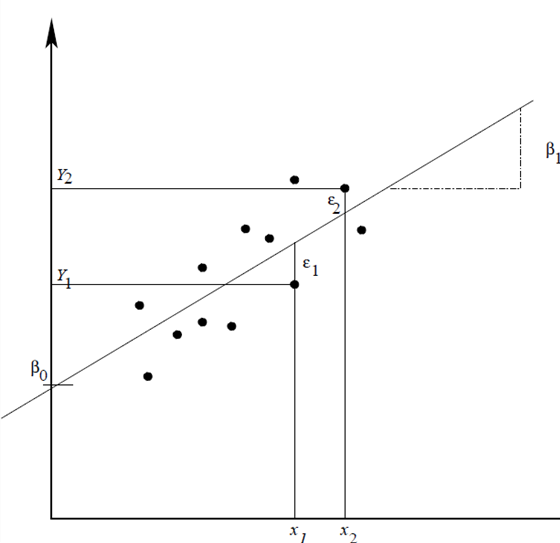
\includegraphics[scale=1]{Chap2-AjusterRLS/Figures/schema_reg_lin}}
\caption[Illustration du modèle de régression linéaire simple]{Illustration du mod\`ele de r\'egression lin\'eaire simple. La droite repr\'esente l'esp\'erance de la
variable endog\`ene, $Y$, en fonction de la valeur de la variable
exog\`ene, $x$. Le param\`etre $\beta_0$ constitue l'ordonn\'ee
\`a l'origine de la droite et le param\`etre $\beta_1$ est égal à la pente de
la droite.}
\label{fig:rls}
\end{figure}


On interprète donc $\beta_0$ comme la valeur moyenne de $Y$ lorsque $x$ vaut zéro et $\beta_1$ comme l'accroissement moyen de $Y$ lorsque $x$ augmente d'une unité. Si $\beta_0 = 0$, l'espérance de $Y$ est nulle lorsque $x$ vaut zéro, et le modèle ne comporte pas d'ordonnée à l'origine. Si $\beta_1 = 0$, l'espérance de $Y$ ne dépend pas de $x$, du moins pas de façon linéaire.

\newpage
\textbf{Modèle centré}

Il arrive que la valeur moyenne de $Y$ lorsque $x$ vaut zéro soit difficile ou inutile à interpréter. On pourra alors utiliser une version centrée du modèle:
\begin{eqnarray*}
 Y_i &=& \beta_0 + \beta_1 x_i + \varepsilon_i \\
 &=& \beta_0^* + \beta_1 (x_i - \overline{x}) + \varepsilon_i \text{ (version centrée)}
\end{eqnarray*}

Dans la version centrée du modèle, l'interprétation de $\beta_1$ est inchangée, mais $\beta_0^*$ s'interprète comme étant la valeur moyenne de $Y$ lorsque $x$ vaut $\overline{x}$. On remarque que $\beta_0^* = \beta_0 + \beta_1 \overline{x}$.


\section{Estimation des paramètres}
\label{sec:estimation}

Dans la régression linéaire simple, on doit estimer trois paramètres: $\beta_0$ et $\beta_1$, qui décrivent la droite de régression, ainsi que $\sigma^2$, la variance des termes d'erreur. Deux approches sont généralement admises pour estimer les paramètres d'un modèle de régression: la méthode des moindres carrés et celle du maximum de vraisemblance. On expliquera comment estimer les paramètres de régression à l'aide de ces deux approches, et on démontrera qu'elles sont équivalentes sous le postulat de normalité $\mathcal{P}_4$.

\subsection{Méthode des moindres carrés}

Tel que mentionné au \autoref{sec:intro}, on attribue généralement la méthode des moindres carrés au mathématicien français Adrien-Marie Legendre (1752-1833). Plusieurs autres mathématiciens de l'époque ont aussi publié des travaux sur le sujet, notamment Carl Friedrich Gauss (1777-1855) et Robert Adrain (1775-1843).

Soit $\hat{Y}_i$ la prévision du modèle pour l'observation $i$, c'est-à-dire la position de $Y_i$ s'il était exactement sur la droite de régression. On appelle résidu la différence entre $Y_i$, la valeur observée de la variable réponse, et cette prévision $\hat{Y}_i$. On le dénote $\hat{\varepsilon}_i$, puisque c'est une estimation du terme d'erreur $\varepsilon_i$.

Avec la méthode des moindres carrés, on cherche à choisir $\hat\beta_0$ et $\hat\beta_1$ de façon à minimiser la somme des carrés des erreurs. On veut donc minimiser la fonction suivante:
\begin{eqnarray}
g(\beta_0,\beta_1) =  \sum_{i=1}^n \varepsilon_i^2  =  \sum_{i=1}^n \left\{Y_i- (\beta_0+\beta_1 x_i)\right\}^2
    \label{eq:MoindresCarres}
\end{eqnarray}

Puisque la fonction \`a minimiser possède de bonnes propri\'et\'es
(entre autres lisse et convexe), elle peut être minimisée en la dérivant par rapport \`a ${\beta}_0$ et ${\beta}_1$, puis en posant ces d\'eriv\'ees \'egales \`a z\'ero. On doit donc résoudre le système d'équations \`a deux inconnues suivant:
\begin{eqnarray}
\left\{ \begin{array}{ccc}
\frac{\partial}{\partial{\beta}_0}
\sum_{i=1}^n(Y_i-{\beta}_0-{\beta}_1 x_i)^2
&=&\label{eq1} 0 \\
\frac{\partial}{\partial{\beta}_1}
\sum_{i=1}^n(Y_i-{\beta}_0-{\beta}_1 x_i)^2
&=&\label{eq2} 0
\end{array}
\right.
\end{eqnarray}

\textbf{Estimation de $\beta_0$}

On dérive d'abord par rapport à $\beta_0$:
\begin{eqnarray*}
 \frac{\partial}{\partial \beta_0} \left\{\sum_{i=1}^n (Y_i - \beta_0 - \beta_1 x_i)^2\right\} &=& \sum_{i=1}^n 2(Y_i - \beta_0 - \beta_1 x_i)(-1)\\
 &=& -2( n \overline{Y} - n \beta_0 - n \beta_1 \overline{x})
\end{eqnarray*}
On pose ensuite cette dérivée égale à zéro, d'où l'apparition des chapeaux, car il s'agit du point critique de la fonction $g(\beta_0,\,\beta_1)$:
\begin{eqnarray}
-2(n \overline{Y} - n \hat\beta_0 - n \hat\beta_1 \overline{x}) & = & 0 \nonumber\\
 \overline{Y} - \hat\beta_0 - \hat\beta_1 \overline{x} & = & 0 \nonumber\\
 \hat\beta_0 & = &  \overline{Y} - \hat\beta_1 \overline{x}
\label{eq:beta0}
\end{eqnarray}


\begin{remarque}
 Il est à noter que l'équation \eqref{eq:beta0} signifie que la droite de régression passe nécessairement par le point de coordonnées $(\overline{x},\overline{Y})$:

\begin{eqnarray}
\overline{Y} = \hat\beta_0+ \hat\beta_1 \overline{x}
 \label{eq:dbeta0egal0}
\end{eqnarray}
\end{remarque}

\textbf{Estimation de $\beta_1$}

On dérive maintenant par rapport à $\beta_1$:
\begin{eqnarray*}
 \frac{\partial}{\partial \beta_1} \left\{\sum_{i=1}^n (Y_i - \beta_0 - \beta_1 x_i)^2\right\} &=& \sum_{i=1}^n 2(Y_i - \beta_0 - \beta_1 x_i)(-x_i)\\
 &=& -2 \left(\sum_{i=1}^n x_i Y_i - \sum_{i=1}^n  \beta_0 x_i - \sum_{i=1}^n  \beta_1 x_i^2 \right).
\end{eqnarray*}

\newpage
En posant cette dérivée égale à zéro et en utilisant  \eqref{eq:beta0}, on a
\begin{eqnarray*}
-2 \left( \sum_{i=1}^n x_i Y_i - \sum_{i=1}^n  \hat\beta_0 x_i - \sum_{i=1}^n  \hat\beta_1 x_i^2\right) & = & 0 \\
\sum_{i=1}^n x_i Y_i &= & \hat\beta_0 \sum_{i=1}^n x_i + \hat\beta_1 \sum_{i=1}^nx_i^2 \\
\sum_{i=1}^n x_i Y_i & = & (\overline{Y}-\hat\beta_1 \overline{x}) \sum_{i=1}^n x_i + \hat\beta_1 \sum_{i=1}^nx_i^2 \\
\sum_{i=1}^n x_i Y_i & = & \overline{Y} \sum_{i=1}^n x_i + \hat\beta_1 \left(\sum_{i=1}^n x_i^2 - \overline{x}\sum_{i=1}^n x_i \right)
\end{eqnarray*}

On obtient donc l'estimateur suivant:
\begin{equation}
\hat{\beta}_1 = \frac{\sum_{i=1}^n x_i Y_i -\overline{Y} \sum_{i=1}^n x_i}{\sum_{i=1}^n x_i^2 - \overline{x}\sum_{i=1}^n x_i}.
\end{equation}


Il est possible ensuite de réécrire $\hat\beta_1$ sous les formes équivalentes suivantes:
\begin{equation*}
 \hat{\beta}_1 =  \frac{\sum_{i=1}^n x_i Y_i - n\overline{x}\overline{Y}}{\sum_{i=1}^n x_i^2 - n\overline{x}^2}
 = \frac{\sum_{i=1}^n (x_i-\overline{x})(Y_i-\overline{Y})}{\sum_{i=1}^n (x_i-\overline{x})^2}
 = \frac{\sum_{i=1}^n (x_i-\overline{x})Y_i}{\sum_{i=1}^n (x_i-\overline{x})^2}
 \label{eq:beta1}
\end{equation*}

Chacune pourra être utile pour calculer $\hat{\beta_1}$ selon le type d'information que nous avons sur les données. On simplifie parfois davantage la notation en écrivant
\begin{equation}
 \hat{\beta}_1  = \frac{S_{xy}}{S_{xx}}
\end{equation}
o\`u
\begin{eqnarray}
S_{xy}=\sum_{i=1}^n (x_i-\overline x)\,Y_i=\sum_{i=1}^nx_iY_i-\frac{1}{n}\left(\sum_{i=1}^n x_i\right)\left(\sum_{i=1}^n Y_i\right)
\label{eq:Sxy}
\end{eqnarray}
\begin{eqnarray}
S_{xx}=\sum_{i=1}^n(x_i-\overline x)^2=\sum_{i=1}^nx_i^2-\frac{1}{n}\left(\sum_{i=1}^n x_i\right)^2
\label{eq:Sxx}
\end{eqnarray}
Il est à noter que $S_{xy}$ et $S_{xx}$ sont appelés respectivement la somme des produits croisés corrigée de $x$ et $Y$ et la somme des carrés corrigée de $x$.


En somme, les estimateurs des moindres carrés pour la RLS sont
\begin{eqnarray}
\hat \beta_1 = \frac{S_{xy}}{S_{xx}} & \hspace{2cm} & \hat\beta_0=\overline{Y} - \hat\beta_1 \overline{x}
\end{eqnarray}


%On ne poursuit pas les développements mathématiques nécessaires pour obtenir ces estimateurs ici. On montrera à la section suivante que la méthode des moindres carrés est équivalente à la méthode du maximum de vraisemblance sous le postulat de normalité, et on montrera alors comment obtenir les estimateurs.

\subsection{Méthode du maximum de vraisemblance}

La méthode du maximum de vraisemblance nécessite de spécifier la distribution exacte des observations $Y_1,\dots, Y_n$. Celle-ci est connue sous l'hypothèse des quatre postulats
\begin{align*}
\mathcal{P}_1. & \; \; \esp[\varepsilon_i]=0 \mbox{ pour } 1\leq i \leq n
&
\mathcal{P}_3. & \; \; \cov(\varepsilon_i,\varepsilon_j)=0 \mbox{ pour } i \neq j \\
\mathcal{P}_2. & \; \; \var[\varepsilon_i]=\sigma^2 \mbox{ pour } 1\leq i \leq n
&
\mathcal{P}_4. & \;\varepsilon_1, \cdots , \varepsilon_n \sim \N(0,\sigma^2)
\end{align*}
En effet, on peut alors écrire le modèle sous la forme
\begin{align*}
Y_i &= \beta_0 + \beta_1 x_i + \varepsilon_i, \ \ \  \varepsilon_i \iid N(0,\sigma^2) \ \ \ \ 1\leq i \leq n
 \end{align*}
ou, de façon équivalente
\begin{equation}
Y_i \sim N(\beta_0 + \beta_1 x_i, \sigma^2)
\end{equation}

La vraisemblance s'exprime donc
\begin{eqnarray*}
 L (\beta_0, \beta_1, \sigma^2)&=&\prod_{i=1} ^n f(Y_i) \\
 &=& \prod_{i=1} ^n \frac{1}{\sqrt{2\pi}\sigma} \exp\left\{-\frac{1}{2} \left(\frac{Y_i-\beta_0 - \beta_1 x_i}{\sigma}\right)^2\right\}.
\end{eqnarray*}

 Il reste ensuite à maximiser la fonction $L (\beta_0, \beta_1)$ ou, plus simplement, son logarithme
 \begin{eqnarray}
 \nonumber l (\beta_0, \beta_1, \sigma^2)&=&\sum_{i=1}^n \left\{-\frac{1}{2}\log(2\pi\sigma^2)-\frac{1}{2\sigma^2}(Y_i - \beta_0 - \beta_1 x_i)^2\right\}\\ \label{eq:MaxVraisemblance}
 &=& -\frac{n}{2} \log (2\pi\sigma^2)-\frac{1}{2 \sigma^2}\sum_{i=1}^n (Y_i - \beta_0 - \beta_1 x_i)^2
\end{eqnarray}

On trouve $\hat\beta_0$, $\hat\beta_1$ et $\hat\sigma^2$ qui minimisent $l (\beta_0, \beta_1,\sigma^2)$ en dérivant respectivement par rapport à $\beta_0,\beta_1$ et $\sigma^2$ puis en posant les dérivées égales à zéro.

%\begin{remarque}
Dans l'équation \eqref{eq:MaxVraisemblance}, on remarque que le premier terme ne contient ni $\beta_0$, ni $\beta_1$. Maximiser la log-vraisemblance par rapport à $\beta_0$ et $\beta_1$ revient donc à maximiser le second terme. Ce dernier étant négatif, cela équivaut à minimiser $\sum_{i=1}^n (Y_i - \beta_0 - \beta_1 x_i)^2$, ce qui correspond exactement à la méthode des moindres carrés de Legendre.  Ainsi, les estimateurs de la méthode du maximum de vraisemblance de $\beta_0$ et $\beta_1$ sont les mêmes qu'avec la méthode des moindres carrés.

La méthode du maximum de vraisemblance présente toutefois certains avantages par rapport à la méthode des moindres carrés. Elle permet notamment d'estimer $\sigma^2$ de façon directe. Ceci permet de trouver la distribution des paramètres et des prévisions et de faire des tests d'hypothèse, comme on verra dans les sections suivantes.
%\end{remarque}

\subsubsection{Estimation de $\sigma^2$}
On estime $\sigma^2$ de la même manière que $\beta_0$ et $\beta_1$ en dérivant le logarithme de la vraisemblance par rapport à $\sigma^2$.
 \begin{eqnarray*}
 \frac{\partial}{\partial \sigma^2}\left\{ -\frac{n}{2} \log (2\pi\sigma^2)-\frac{1}{2 \sigma^2}\sum_{i=1}^n (Y_i - \beta_0 - \beta_1 x_i)^2\right\}
 & = & -\frac{n}{2} \frac{1}{2\pi\sigma^2} 2\pi + \frac{1}{\sigma^4} \frac{1}{2}\sum_{i=1}^n(Y_i-\beta_0-\beta_1 x_i)^2 \\
 & = & -\frac{n}{2\sigma^2}+ \frac{1}{2 \sigma^4}\sum_{i=1}^n(Y_i-\beta_0-\beta_1 x_i)^2
\end{eqnarray*}

En posant la dérivée égale à zéro et en remplaçant les paramètres $\beta_0$ et $\beta_1$ par leurs estimateurs, on a :
\begin{equation}
 \hat{\sigma}^2_{MV} = \frac{1}{n}\sum_{i=1}^n(Y_i - \hat{\beta_0} - \hat{\beta_1}x_i)^2 = \frac{1}{n}\sum_{i=1}^n \hat{\varepsilon_i}^2
 \label{sigma2}
\end{equation}

Rappelons que $\hat{\varepsilon_i}$ désigne l'estimation du terme d'erreur, que l'on nomme résidu.

\section{Exemple}
\label{exemple-RLS-interpretation}
Le petit exemple qui va servir de fil conducteur pour les chapitres sur la régression linéaire simple est tiré de \citet[Exemple 13.1, page 367]{Hin_Mon_Gol_Bor:05}. Un ingénieur chimiste a analysé l'effet de la température de fonctionnement d'un procédé sur le rendement du produit. Les valeurs obtenues sont résumées ci-dessous.


\begin{table}[!ht]
\caption{10 mesures du rendement en $\%$ en fonction de la température en $^{\circ}\mathrm{C}$ } \label{tab:donnees_exp}
\label{exp:donnees}
\begin{tabular}{r|rrrrrrrrrr}
Température [$^{\circ}\mathrm{C}$] & 100 & 110 & 120 & 130 & 140 & 150 & 160 & 170 & 180 & 190 \\[6pt] \hline
\\[-6pt]
Rendement [$\%$] & 45 & 51 & 54 & 61 & 66 & 70 & 74 & 78 & 85 & 89
\end{tabular}
\end{table}

\begin{figure}[h!]
\centering
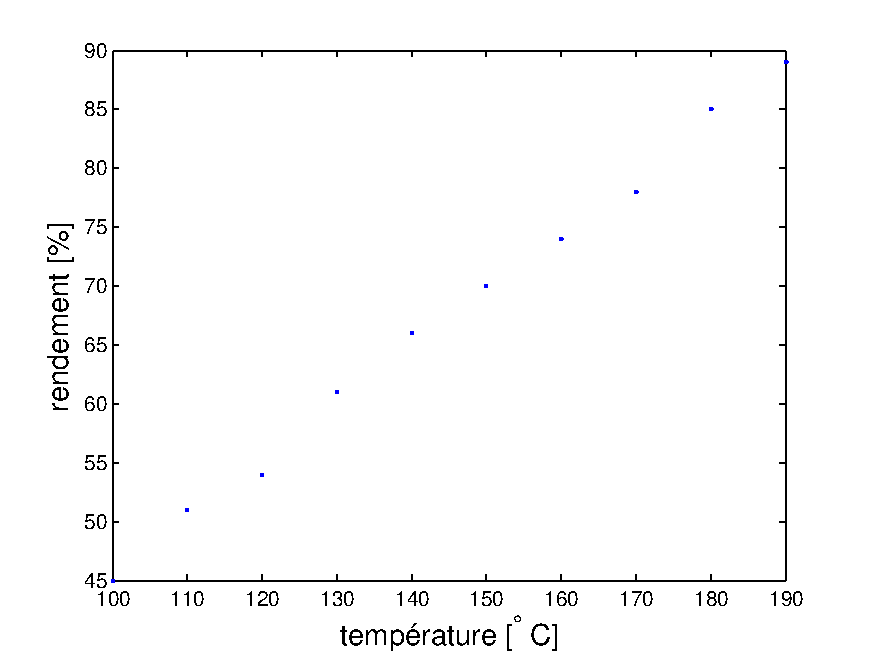
\includegraphics[scale=0.6]{Chap2-AjusterRLS/Figures/scatter_plot_exp.pdf}
\caption{Diagramme de dispersion du rendement en fonction de la température}
\label{fig:scatter_plot_exp}
\end{figure}

On peut constater sur la figure \ref{fig:scatter_plot_exp} qu'il existe une relation forte entre le rendement et la température. On va supposer que cette relation est linéaire et donc modéliser ces données à l'aide de l'équation \eqref{eq:reg_lin_simple}. On calcule d'abord
\begin{align*}
 \sum_{i=1}^{10} x_i &=1450 &\hspace{1cm} & \overline{x}= \frac{1}{10} \sum_{i=1}^{10} x_i=145 & \sum_{i=1}^{10} x_i^2 = 218~500\\
  \sum_{i=1}^{10} y_i&=673 &\hspace{1cm} & \overline{y}= \frac{1}{10} \sum_{i=1}^{10} y_i=67,3 & \sum_{i=1}^{10} Y_ix_i= 101~570
\end{align*}
On obtient alors
\vspace{-0.1 in}
\begin{align*}
S_{xx}&=218~500-(1450)^2/10=8250 \\
S_{xy}&=101~570-1450\times 673/10=3985
\end{align*}
Et donc
\vspace{-0.1 in}
\begin{align*}
\hat{\beta_1} &= 3985/8250=0,483 \\
\hat{\beta_0} &= 67,3-0,483\times145=-2,739
\end{align*}
Le modèle de régression linéaire simple ajusté devient alors $\hat Y_i=-2,739+0,483x_i$. Ainsi, une augmentation de un degré Celsius de la température du procédé est associée à une augmentation moyenne de $0,483$ point de pourcentage du rendement du produit. Le modèle indique aussi qu'à une température nulle, le rendement attendu est de $-2,739\%$.

La figure~\ref{fig:reg_lin_exp} montre l'ajustement obtenu sous forme d'une droite. Dans ce cas-ci la relation linéaire semble très appropriée pour modéliser la relation entre les variables, mais ce ne sera pas toujours le cas.

\begin{figure}[h!]
\centering
\includegraphics[scale=0.6]{Chap2-AjusterRLS/Figures/reg_lin_exp}
\caption{Diagramme de dispersion du rendement en fonction de la température avec la droite de régression estimée superposée}
\label{fig:reg_lin_exp}
\end{figure}

On peut également estimer $\sigma^2$ à partir des données. Il faut d'abord calculer la valeur prédite et le résidu pour chacune des observations, comme au Tableau \ref{tab:cal_sigma2_exp}. L'équation~\eqref{sigma2} livre alors
$$\hat{\sigma}^2_{MV}=\frac{1}{10} \{(-0,561)^2+\cdots+(-0,0301)^2\}=\frac{7,224}{10}=0,7224.$$

\begin{table}[h!]
\caption{Tableau résumant $x_i$, $Y_i$, $\hat Y_i$ et $\hat\varepsilon_i$, $i=1,\dots,10$ pour le calcul de $\hat\sigma^2_{MV}$ dans l'exemple de la section \ref{exemple-RLS-interpretation}}
\label{tab:cal_sigma2_exp}
\begin{center}
\begin{tabular}{c|cccc}
\centering
$i$ & $x_i$& $Y_i$ & $\hat Y_i$ & $\hat\varepsilon_i$ \\ \hline
1 & 100 & 45 & 45,561 &  -0,561 \\
2 & 110  & 51  & 50,391 & 0,609 \\
3 &  120 & 54  & 55,221 & -1,221 \\
4 & 130  & 61 & 60,051 & 0,949\\
5 & 140 & 66  & 64,881  &  1,119 \\
6 & 150  & 70 & 69,711  & 0,289\\
7 &160  & 74 & 74,541 & -0,541\\
8 & 170  & 78 & 79,371 & -1,371\\
9 & 180 & 85 & 84,201 & 0,799\\
10 & 190  & 89 & 89,031 & -0,031
\end{tabular}
\end{center}
\end{table}


\chapter{Inférence pour la RLS}
\label{sec:InferenceRLS}

\section{Inférence sur les paramètres}
\label{sec:InférenceParamètres}

On a montré comment obtenir des estimations pour les différents paramètres du modèle de régression linéaire simple. On souhaite en général également faire de l'inférence sur les vraies valeurs des paramètres $\beta_0$, $\beta_1$ et $\sigma^2$. Pour ce faire, on utilisera la distribution des estimateurs, que nous dérivons ici.

\subsection{Distribution des estimateurs}
\label{sec:LoisBetas}

\subsubsection{Distribution de $\hat{\beta}_1$}
\label{sec:LoiDeHatBeta1}

%Notez que $\hat{\beta}_1$ est une variable aléatoire puisque c'est une fonction des $Y_i$ qui sont elles-mêmes des variables aléatoires. On veut trouver sa distribution.

On note d'abord que $\hat{\beta}_1$ constitue une combinaison linéaire des $Y_i$. En effet,
$$ \hat{\beta}_1= \frac{\sum_{i=1}^n (x_i-\overline{x})Y_i}{\sum_{i=1}^n (x_i-\overline{x})^2} = \sum_{i=1}^n a_i Y_i
$$
o\`u $a_i= \{(x_i-\overline{x})/\sum_{i=1}^n(x_i-\overline{x})^2\} = (x_i-\overline{x})/S_{xx}$.

Étant donné qu'une combinaison linéaire de variables aléatoires normales suit également une distribution normale, il s'ensuit que $\hat\beta_1$ est distribué selon une loi normale. Il ne reste qu'à trouver l'espérance et la variance de celle-ci.

Notons d'abord que
 \begin{eqnarray*}
 \sum_{i=1}^n a_i & = & \frac{\sum_{i=1}^n(x_i-\overline{x})} {S_{xx}} = 0 \\
\sum_{i=1}^n a_i x_i & = & \frac{\sum_{i=1}^n(x_i-\overline{x})x_i } {S_{xx}} =\frac{\sum_{i=1}^n(x_i-\overline{x})(x_i-\overline{x})}{S_{xx}}=\frac{S_{xx}}{S_{xx}}=1.
\end{eqnarray*}




Pour l'espérance, on peut montrer que $\hat{\beta}_1$ est un estimateur sans biais de $\beta_1$:
\begin{eqnarray*}
 \esp[\hat{\beta}_1] &=& \sum_{i=1}^n a_i \esp[Y_i] \\
 &=& \sum_{i=1}^n a_i (\beta_0 + \beta_1 x_i)\\
 &=& \beta_0 \sum_{i=1}^n a_i + \beta_1 \sum_{i=1}^n a_i x_i\\
 &=& \beta_1
\end{eqnarray*}


Pour la variance de $\hat\beta_1$, on peut calculer
\begin{eqnarray*}
 \var[\hat\beta_1]&=&\var\left[\sum_{i=1}^n a_i Y_i\right]\\
 &=& \sum_{i=1}^n a_i ^2 \var[Y_i]\\
 &=& \sum_{i=1}^n \frac{(x_i-\overline{x})^2}{S_{xx}^2} \var[Y_i]\\
 &=& \frac{1}{S^2_{xx}} \sum_{i=1}^n (x_i-\overline{x})^2 \var[Y_i]\\
 &=& \frac{S_{xx}}{S_{xx}^2} \sigma^2 \\
 &=& \frac{\sigma^2}{S_{xx}}
\end{eqnarray*}

On obtient donc la distribution de $\hat\beta_1$ suivante
\begin{eqnarray}
\label{distbeta1}
 \hat{\beta}_1 \sim N\left( \beta_1, \frac{\sigma^2}{S_{xx}} \right).
 \label{loibeta1}
\end{eqnarray}

\vspace{0.1in}
\begin{remarque}
Seulement certaines hypothèses de la RLS ont été nécessaires pour calculer cette distribution. Lesquelles? Et que nous indique la forme de cette distribution sur l'estimation de la pente dans un modèle de régression linéaire simple?
\end{remarque}


\subsubsection{Distribution de $\hat\beta_0$}
\label{DistributionBeta0}
L'estimateur $\hat\beta_0$ peut également s'exprimer comme une combinaison linéaire des $Y_i$ :
\begin{eqnarray*}
 \hat{\beta}_0 &=& \overline{Y} - \hat{\beta}_1 \overline{x} \\
 &=& \sum_{i=1}^n Y_i /n - \overline{x} \sum_{i=1}^n a_i Y_i \\
 &=& \sum_{i=1}^n (1/n - a_i \overline{x}) Y_i
\end{eqnarray*}
Par le même raisonnement que pour $\hat\beta_1$, on a donc que $\hat\beta_0$ est distribué selon une loi normale. On peut calculer la moyenne et la variance de cette loi en utilisant l'espérance et la variance de $\hat\beta_1$. Pour l'espérance, on a que
\begin{eqnarray*}
 \esp[\hat{\beta}_0] &=& \esp[\overline{Y} - \hat{\beta}_1 \overline{x}] \\
 &=& \frac{1}{n}\sum_{i=1}^n \esp[Y_i] - \overline{x} \esp[\hat{\beta}_1]  \\
 &=& \frac{1}{n}\sum_{i=1}^n(\beta_0+\beta_1 x_i)-\overline{x}\beta_1 \\
 & = & \beta_0+\beta_1 \overline x-\beta_1\overline x \\
 & = & \beta_0
\end{eqnarray*}
La variance s'exprime quant à elle de la façon suivante
\begin{eqnarray*}
 \var[\hat{\beta}_0] &=& \var[\overline{Y} - \hat{\beta}_1 \overline{x}] \\
 &=& \var\left[\frac{1}{n}\sum_{i=1}^n Y_i\right]+ \overline{x}^2 \var[\hat{\beta}_1]-2\overline x\cov[\overline Y,\hat\beta_1]  \\
 &=& \frac{\sigma^2}{n}+\overline{x}^2\frac{\sigma^2}{S_{xx}} \\
 & = & \sigma^2\left(\frac{1}{n}+\frac{\overline{x}^2}{S_{xx}}\right)
\end{eqnarray*}
Pour obtenir l'expression finale pour cette variance, il faut démontrer que $\cov[\overline Y,\hat\beta_1]=~0$, ce qui est laissé en exercice. \\

On obtient ainsi la loi suivante pour $\hat\beta_0$:
\begin{eqnarray}
\label{distbeta0}
 \hat{\beta_0} \sim \N\left\{\beta_0, \left(\frac{1}{n}+\frac{\overline{x}^2}{S_{xx}}\right)\sigma^2\right\}.
\label{loibeta0}
\end{eqnarray}

\begin{exemple}
Calculons la variance de $\hat\beta_0$ et $\hat\beta_1$ dans l'exemple de la section \ref{exemple-RLS-interpretation}. On doit pour ce faire connaître la valeur de la variance des termes d'erreur. Supposons ici que $\sigma^2=1$. On sait déjà que $n=10,\overline x=145$ et $S_{xx}=8250$. Par conséquent on a
$$\var[\hat\beta_0]=\left( \frac{1}{10}+\frac{145^2}{8250} \right)(1)=2,648$$
$$\var[\hat\beta_1]=\frac{1^2}{8250}=1,212\times 10^{-4}.$$
\end{exemple}



\subsection{Intervalles de confiance pour $\beta_0$ et $\beta_1$}
\label{sec:IntervallesDeConfiance}

On peut utiliser les distributions de $\hat{\beta_0}$ et $\hat{\beta_1}$ pour construire des intervalles de confiance pour $\beta_0$ et $\beta_1$ avec la méthode des pivots. Par exemple, pour un intervalle de confiance pour $\beta_1$, on centre et réduit la variable aléatoire pour obtenir
\begin{equation}
\frac{\hat{\beta}_1-\beta_1}{\sqrt{\sigma^2/S_{xx}}}\sim \N(0,1).
\label{disbeta0std}
\end{equation}
%équations \eqref{distbeta0} et \eqref{distbeta1})
\vspace{-0.05 in}
Si $\sigma^2$ était connue, un intervalle de confiance de niveau $100(1-\alpha)\%$ serait donc donné par $$[\hat{\beta_1}\pm z_{1-\alpha/2} \sigma / \sqrt{S_{xx}}].$$ Or, $\sigma^2$ n'est généralement pas connue et on doit par conséquent l'estimer. L'estimateur du maximum de vraisemblance de cette quantité est $\sum_{i=1}^n \hat{\varepsilon}_i^2 /n$ mais ce dernier est biaisé.
%Montrer que c'est le cas.
On utilisera donc plutôt l'estimateur non biaisé défini par $$\hat{\sigma}^2=  \frac{1}{n-2} \sum_{i=1}^n \hat{\varepsilon}_i^2.$$

\vspace{-0.05 in}
Remplacer $\sigma^2$ par $\hat\sigma^2$ dans le terme de gauche de \ref{disbeta0std} a toutefois pour conséquence que cette variable aléatoire ne suit plus une loi normale. On peut néanmoins montrer, en utilisant des notions de statistique mathématique, que
\begin{equation}
 \frac{\frac{\hat{\beta}_1-\beta_1}{\sigma/\sqrt{S_{xx}}}}
 {  \sqrt{\frac{\hat\sigma^2}{\sigma^2} } } \sim \mathcal{T}_{n-2}.
\label{disbeta0stds}
\end{equation}


On peut alors déduire un intervalle de confiance de niveau $100(1-\alpha)\%$ pour $\beta_1$:
\begin{eqnarray}
\left[\hat{\beta}_1 \pm t_{n-2; 1-\alpha/2} \left(\frac{\hat\sigma}{\sqrt{S_{xx}}}\right)\right],
\end{eqnarray}
où $t_{n-2; 1-\alpha/2}$ dénote le $(1-\alpha/2)$-ième quantile d'une loi $\mathcal{T}$ à $(n-2)$ degrés de liberté.\\

 Il est possible de construire de la même manière un intervalle de confiance pour $\beta_0$. On obtient alors l'intervalle de confiance suivant:
 \begin{eqnarray}
\left[\hat{\beta}_0\pm t_{n-2; 1-\alpha/2}\; \hat\sigma\sqrt{{1\over n}+{\overline{x}^2\over S_{xx}}}\right].
\label{ci:beta0}
\end{eqnarray}

\vspace{0.05in}
\begin{remarque}
Pour trouver \ref{disbeta0stds}, on note que
\begin{eqnarray*}
 \frac{\frac{\hat{\beta}_1-\beta_1}{\sigma/\sqrt{S_{xx}}}}{\sqrt{\frac{\sum_{i=1}^n \hat{\varepsilon}_i^2}{\sigma^2 (n-2)}}}=\frac{U}{\sqrt{V/\nu}}
\end{eqnarray*}
où $U=\frac{\hat{\beta}_1-\beta_1}{\sigma/\sqrt{S_{xx}}}$ est distribué selon une loi normale centrée réduite et $V=\frac{\sum_{i=1}^n \hat{\varepsilon}_i^2}{\sigma^2}$ suit une loi du khi-carré à $\nu=(n-2)$ degrés de liberté, puisque c'est une somme du carré de variables aléatoires normales.
Comme il s'agit d'un rapport entre une variable aléatoire normale centrée réduite et la racine carrée d'une variable khi-carré divisée par son degré de liberté  $(n-2)$, on obtient la distribution d'une loi $\mathcal{T}$ de Student à $(n-2)$ degrés de liberté ($\mathcal{T}_{n-2}$):
\begin{eqnarray*}
 \frac{\frac{\hat{\beta}_1-\beta_1}{\sigma/\sqrt{S_{xx}}}}{\sqrt{\frac{\sum_{i=1}^n \hat{\varepsilon}_i^2}{\sigma^2 (n-2)}}} \sim \frac{\N(0,1)}{\sqrt{\chi_{n-2}^2/(n-2)}} \sim \mathcal{T}_{n-2}
 \end{eqnarray*}
\end{remarque}

\vspace{0.1in}
\begin{exemple}
\label{exp:int_beta}
Calculons un intervalle de confiance pour $\beta_0$ et $\beta_1$ avec les données de la section \ref{exemple-RLS-interpretation}. La plupart des quantités nécessaires ont déjà été calculées. Il ne manque que
$$\hat\sigma=\sqrt{\frac{1}{10-2} \sum_{i=1}^{10}\hat\varepsilon_i^2}=\sqrt{\frac{7,224}{8}}=0,950.$$
Si on fixe $\alpha=5\%$, il faut calculer $t_{n-2; 0,975}$. On peut trouver dans une table que ce quantile est  $t_{8;0,975}=2,306$. On obtient alors les intervalles suivants:
$$[\hat{\beta}_0\pm 2,306\times0,950\sqrt{1/10+145^2/8250}]=[\hat{\beta}_0\pm 3,566]=[-6,305;0,827]$$
$$[\hat{\beta}_1\pm 2,306\times 0,950/\sqrt{8250}]=[\hat{\beta}_1\pm 0,024]=[0,459;0,507]$$

\end{exemple}

\newpage
\subsection{Tests d'hypothèses}

On peut également se baser sur les distributions trouvées à la section \ref{sec:LoisBetas}
pour mettre en {\oe}uvre des tests d'hypothèse sur la valeur des coefficients.

L'hypothèse la plus souvent testée concerne la nullité de la pente, à savoir $\mathcal{H}_0: \beta_1 = 0$. Sous $\mathcal{H}_0$, $\frac{\hat{\beta}_1}{\hat\sigma/\sqrt{S_{xx}}} \sim \mathcal{T}_{n-2}$ et $\prob(|t_{n-2}|>|t_{\text{obs}}|)$, où $t_{\text{obs}}$ désigne la statistique du test calculée, nous livre la $p$-valeur du test bilatéral. Si la $p$-valeur est plus petite que le seuil $\alpha$ choisi, on rejette l'hypothèse nulle que $\beta_1=0$. Au contraire, si la $p$-valeur est supérieure au seuil, on ne peut pas rejeter l'hypothèse nulle que $\beta_1=0$.


 Dans le cas où l'hypothèse nulle que l'ordonnée à l'origine $\beta_0=0$ ne peut être rejetée, le modèle peut se simplifier :  $Y_i = \beta_1 x_i + \varepsilon_i$.

\begin{exemple}
Toujours avec les données de la section \ref{exemple-RLS-interpretation}, on trouve
$$ t_{obs} = \frac{\hat{\beta_1}}{\hat\sigma/\sqrt{S_{xx}}} = \frac{0,483}{0,950/\sqrt{8250}} = 46,17 $$
Un logiciel nous permet d'obtenir $5.35 \times 10^{-11}$ comme valeur de $p$ correspondante. On rejette donc l'hypothèse d'une pente nulle. Notez qu'on aurait pu arriver à la même conclusion simplement à l'aide de l'intervalle de confiance construit à l'exemple \ref{exp:int_beta}. En effet, l'intervalle de confiance à 95\% pour $\beta_1$ ne contient pas la valeur de $0$, ce qui permet de rejeter l'hypothèse que $\beta_1 = 0$ au seuil $\alpha = 0.05$.

%Il est à souligner que comme 0 appartient à l'intervalle de confiance pour $\beta_0$, on ne peut pas rejeter l'hypothèse nulle que l'ordonnée à l'origine soit égale à zéro. Le modèle peut donc être simplifié.
\end{exemple}


\section{Prévision}
\label{sec:PrévisionRLS}

On a déjà défini $\hat{Y}_i = \hat{\beta}_0 + \hat{\beta}_1 x_i$, la prévision du modèle en $x_i$. On souhaite maintenant obtenir un intervalle de confiance pour cette valeur.

On doit alors distinguer deux cas:
\begin{enumerate}
\item[(i)] Estimer $\esp[Y|x=x_0]$, la valeur moyenne de $Y$ prédite par le modèle pour une valeur $x=x_0$
de la variable exog\`ene.
\item[(ii)] Estimer la valeur d'une observation/r\'ealisation de $Y$ lorsque
la variable exog\`ene prend la valeur $x_0$. Cette valeur sera dénotée par ${Y}_0^*$.
\end{enumerate}

Dans le premier cas, on souhaite estimer la valeur de la droite en $x_0$, alors que dans le deuxième cas on s'intéresse à une réalisation de la variable dépendante, qui ne sera pas nécessairement sur la droite. L'intervalle de confiance sera plus grand dans le deuxième cas, pour tenir compte de la variabilité additionnelle causée par la fluctuation aléatoire autour de la droite.
%Les détails sont présentés plus bas.

\subsection{Prévision de la valeur moyenne $\esp[Y|x=x_0]$}

Soit $\esp[Y|x=x_0]$, la valeur moyenne de $Y$ prédite par le modèle lorsque $x=x_0$. Cette quantité est estimée par $\hat{Y}_0 = \hat{\beta}_0 + \hat{\beta}_1 x_0$.
On utilise le fait que $Y_i \sim \N(\beta_0+\beta_1x_i,\sigma^2)$ pour trouver la distribution de $\hat{Y}_0$.
On exprime d'abord $\hat{Y}_0$ sous la forme d'une combinaison linéaire des $Y_i$ de la façon suivante:
\begin{eqnarray*}
 \hat{Y}_0 &=& \hat{\beta}_0 + \hat{\beta}_1 x_0 \\
 &=&\sum_{i=1}^n (1/n - a_i \overline{x}) Y_i + \left(\sum_{i=1}^n a_i Y_i\right) x_0 \\
 &=& \sum_{i=1}^n (1/n - a_i \overline{x} + a_i x_0) Y_i\\
 &=& \sum_{i=1}^n c_i Y_i
\end{eqnarray*}
où
 \[c_i = 1/n - a_i \overline{x} + a_i x_0.\]

On peut montrer que $\sum_{i=1}^n c_i = 1$, que $\sum_{i=1}^n c_i x_i = x_0$ et que $\sum_{i=1}^n c_i^2 = \frac{1}{n} + \left\{\frac{(\overline{x}-x_0)^2}{S_{xx}}\right\}$.

On peut ensuite en déduire que
\begin{eqnarray}
 \esp[\hat{Y}_0]= \sum_{i=1}^n c_i \esp[Y_i]= \sum_{i=1}^n c_i (\beta_0 + \beta_1 x_i) = \beta_0 + \beta_1 x_0 \\
 \label{eq:varyo}
 \var[\hat{Y}_0]= \sum_{i=1}^n c_i^2 \var[Y_i] = \left\{ \frac{1}{n} + \frac{(\overline{x}-x_0)^2}{S_{xx}}\right\} \sigma^2
\end{eqnarray}

Puisque $\hat{Y}_0$ est une combinaison linéaire des $Y_i$, qui suivent une loi normale, $\hat{Y}_0$ suit lui-même une loi normale. On a donc

\begin{equation}
\hat{Y}_0 \sim \N\left(\beta_0 + \beta_1 x_0, \left\{ 1/n + \frac{(\overline{x}-x_0)^2}{S_{xx}}\right\} \sigma^2 \right).
\end{equation}

À partir de ce résultat, il est possible de calculer un intervalle de confiance autour de la valeur moyenne prédite en remplaçant $\sigma^2$ par son estimateur $\hat\sigma^2$. En utilisant le même raisonnement qu'à la section \ref{sec:IntervallesDeConfiance}, on obtient l'intervalle de confiance de niveau $1-\alpha$ suivant pour $\esp[Y|x=x_{0}]$:
\begin{eqnarray}
\left[(\hat{\beta}_0 + \hat{\beta}_1 x_0)\; \pm\; t_{n-2; 1-\alpha/2} \;\hat\sigma \; \sqrt{\frac{1}{n}+\frac{(\overline x-x_0)^2}{S_{xx}}}\right]
\label{eq:int_conf_val_moy_prev}
\end{eqnarray}

 \subsection{Prévision d'une observation $Y_0^*$ lorsque $x=x_0$}

Il est important de comprendre que l'intervalle de confiance défini à l'équation \eqref{eq:int_conf_val_moy_prev} concerne la moyenne de $Y$ au point $x=x_0$. Pour construire ce qu'on appelle un intervalle de prévision, il faut considérer à la fois la variance liée au modèle (à l'estimation des paramètres) et la variance liée à la variabilité naturelle du phénomène, c'est-à-dire la variance du terme d'erreur ($\varepsilon$). Or, l'équation \eqref{eq:varyo} ne tient pas compte de la variance du terme d'erreur, qui est égale à $\sigma^2$.

Désignons la prévision de la moyenne de $Y$ en  $x_0$ par $\hat{Y}_0 = \hat{\beta}_0 + \hat{\beta}_1 x_0$ et la prévision d'une observation individuelle par $\hat{Y}_0^* = \hat{\beta}_0 + \hat{\beta}_1 x_0 + \varepsilon$. L'espérance de $\hat{Y}_0$ et celle de $\hat{Y}_0^*$ sont égales parce que l'espérance des termes d'erreur est nulle. Ce n'est pas le cas des variances.

On trouve en effet que
\begin{eqnarray}
 \var[\hat{Y}_0^*] &=& \var[\hat{Y}_0] + \var [\varepsilon] \nonumber\\
 &=&\left\{ \frac{1}{n} + \frac{(\overline{x}-x_0)^2}{S_{xx}}\right\} \sigma^2 + \sigma^2 \nonumber\\
 &=& \left\{1+\frac{1}{n} + \frac{(\overline{x}-x_0)^2}{S_{xx}} \right\} \sigma^2.
 \label{eq:varyo*}
\end{eqnarray}

Le méthode de calcul de l'intervalle de prévision de niveau $1-\alpha$ pour ${Y}_0^*$ est similaire à celle de l'intervalle de confiance pour  $\esp[Y|x=x_0]$. On obtient donc
\begin{eqnarray}
\left[(\hat{\beta}_0 + \hat{\beta}_1 x_0)\; \pm\; t_{n-2; 1-\alpha/2} \; \hat\sigma \; \sqrt{1+\frac{1}{n}+\frac{(\overline x-x_0)^2}{S_{xx}}} \right].
\label{eq:int_prev}
\end{eqnarray}


En analysant les formules \eqref{eq:varyo} et \eqref{eq:varyo*}, nous constatons que les variances diminuent lorsque $n$ augmente ou que $S_{xx}$ augmente. Cela signifie que plus la taille de l'échantillon est grand et/ou plus il y a de la variabilité dans les valeurs de la variable exogène, plus les estimations seront précises. Au contraire, plus le point $x_0$ pour lequel une prévision est requise est éloigné du centre $(\overline x)$ des variables explicatives, plus la prévision sera imprécise.
Il est important de prendre ces remarques en considération lors de la planification des expériences.


\begin{remarque}
L'intervalle de prévision pour $Y_0^*$ sera toujours plus large que l'intervalle de confiance pour $\esp[Y|x=x_0]$. Pour cette raison, il peut arriver dans la pratique qu'un client préfère présenter l'intervalle de confiance plutôt que l'intervalle de prévision. Il est important de bien comprendre et de bien expliquer la distinction entre les deux intervalles pour éviter une mauvaise interprétation des résultats.
\end{remarque}


\begin{exemple}
On désire calculer un intervalle de confiance à 95 $\%$ pour le rendement moyen du produit ($\esp[Y|x=x_0]$) lorsque la température de fonctionnement est de 150 $^{\circ}\mathrm{C}$ et pour le rendement d'un produit spécifique (${Y}_0^*$) lorsque la température est de 150 $^{\circ}\mathrm{C}$.

Dans les deux cas, la prévision est $\hat\beta_0+ \hat\beta_1\times150 =-2,739+0,483\times 150=69,711 \%$.

La plupart des quantités nécessaires au calcul des deux intervalles ont été déjà calculées auparavant. On tire de la section \ref{exemple-RLS-interpretation}  que $\overline x=145, S_{xx}=8250$ et de l'exemple \ref{exp:int_beta} que $\hat\sigma=0,950$ et que $t_{8; 0,975}=2,306$. Il nous reste seulement à calculer $(x_0-\overline x)^2=(150-145)^2=25$.

En utilisant l'équation \eqref{eq:int_conf_val_moy_prev}, on obtient l'intervalle de confiance du rendement moyen :
$$[69,711\pm 2,306\times 0,950\times\sqrt{1/10+25/8250}]=[69,711 \pm 0,703]=[69,008;70,414].$$

L'intervalle de prévision du rendement d'un produit quelconque, appelé également intervalle de prévision, se calcule par l'équation~\eqref{eq:int_prev}: \\
 $[69,711\pm 2,306\times 0,950\times\sqrt{1+1/10+25/8250}]=[69,711\pm 2,301]=[67,410;72,012]$.

Comme on l'a déjà signalé l'intervalle de prévision est plus large que l'intervalle de confiance pour $\esp[Y|x=150]$.
\end{exemple}


\section{Analyse de la variance}
\label{sec:AnalyseDeLaVariance}

L'analyse de la variance est vue en profondeur dans un cours qui lui est dédié, mais c'est un outil qui peut également être utile dans une analyse de régression. On verra dans cette section comment la variabilité dans les observations de la variable endogène $Y_1,\ldots,Y_n$ peut se décomposer sous le modèle de régression linéaire. Cette décomposition constitue la base des tests d'ajustement du modèle.

\subsection{Décomposition de la variabilité}

On note d'abord que les valeurs de la variable réponse ne seront pas toutes identiques dans le jeu de données. Une partie de la différence entre les $Y_i$ peut être expliquée par la différence entre les $x_i$, puisque selon le modèle de régression la variable réponse est expliquée en partie par la variable explicative. Il restera toutefois une partie de la variabilité des $Y_i$ qui n'est pas expliquée par les différences dans les valeurs de $x_i$. Mathématiquement, on peut écrire
\begin{align*}
Y_i - \overline{Y} &= (\hat{Y}_i - \overline{Y})  +  (Y_i - \hat{Y}_i)
\end{align*}
La base de l'analyse de variance en régression, c'est que la même relation est vraie au niveau de la somme des carrés totaux:
\begin{eqnarray*}
  \sum_{i=1}^n (Y_i-\overline{Y})^2 & = & \sum_{i=1}^n (Y_i - \hat{Y}_i + \hat{Y}_i - \overline{Y})^2\\
 &=&  \sum_{i=1}^n (Y_i - \hat{Y}_i)^2 + \sum_{i=1}^n(\hat{Y}_i - \overline{Y})^2 + 2\sum_{i=1}^n (Y_i-\hat{Y}_i)(\hat{Y}_i-\overline{Y})\\
 &=&  \sum_{i=1}^n (Y_i - \hat{Y}_i)^2 + \sum_{i=1}^n(\hat{Y}_i - \overline{Y})^2.
\end{eqnarray*}

\vspace{-0.05 in}
On écrira plus simplement
\begin{equation}\label{eq:decompvar}
SC_{tot}=SC_{reg}+SC_{res}.
\end{equation}
o\`u
\vspace{-0.05 in}
\begin{align*}
SC_{tot}& =\sum_{i=1}^n(Y_i-\overline{Y})^2 \; , \mbox{ la somme des carrés totale}, \\
SC_{reg} & =\sum_{i=1}^n(\hat{Y}_i-\overline{Y})^2 \; \mbox{ la somme des carrés de la régression, et}\\
SC_{res}&=\sum_{i=1}^n(Y_i-\hat{Y}_i)^2 \; \mbox{ la somme des carrés résiduelle.}
\end{align*}
La somme des carr\'es totaux $SC_{tot}$ quantifie la variabilit\'e dans les $Y_i$ autour de leur valeur moyenne.  La somme des carrés de la régression $SC_{reg}$ quantifie la variabilit\'e dans les prévisions $\hat{Y}_i$. Étant donné que les $\hat{Y}_i$ ne varient qu'avec les $x_i$, cette somme de carrés est la partie de la variabilit\'e dans les $Y_i$ expliqu\'ee par le fait que toutes les observations n'ont pas la m\^eme valeur pour $x_i$. La somme  des carrés résiduelle $SC_{res}$ mesure la variabilit\'e dans les $(Y_i-\hat{Y}_i)$. Cette variabilit\'e est induite par le fait que la valeur de $Y_i$ n'est pas expliqu\'ee parfaitement par le mod\`ele de
r\'egression.

%Cette variabilit\'e se d\'ecompose en deux parties : la somme des carrés de la régression ($SC_{reg}$) et la somme des carrés résiduelle ($SC_{res})$.

\begin{exemple}
\label{exp:ss}
Toujours dans l'exemple du rendement d'un produit en fonction de la température de fonctionnement du procédé, on peut calculer que
{\small
\begin{align*}
SC_{tot} &= \sum_{i=1}^n(Y_i-\overline{Y})^2 = 1931,2 \\
SC_{res} &= \sum_{i=1}^n(Y_i-\hat{Y}_i)^2 = (n-2)*\hat\sigma^2 = 7,224 \\
SC_{reg} &= \sum_{i=1}^n(\hat{Y}_i-\overline{Y})^2 = 1924,876
\end{align*}
}
On vérifie alors que $SC_{tot} = SC_{reg} + SC_{res}$. On note que la température \`a elle seule ne peut pas expliquer en totalit\'e pourquoi toutes les expériences ne possèdent pas le m\^eme rendement.
\end{exemple}

\subsection{Test global de la régression}

La somme des carrés de la régression ($SC_{reg}$) constitue donc la portion de la variance expliquée par le modèle, alors que la somme des carrés résiduelle ($SC_{res}$) représente la partie que le modèle n'explique pas. Intuitivement, on comprend que si la proportion de la variance expliquée par le modèle ($SC_{reg}/SC_{tot}$) est élevée, le modèle est bon.

L'analyse de la variance utilise cette idée pour effectuer un test global de la régression. On désire tester les hypothèses suivantes
\begin{align}
H_0&:Y_i=\beta_0+\varepsilon_i \nonumber \\
H_1&:Y_i=\beta_0+\beta_1x+\varepsilon_i  \label{eq:HypotheseAnova}
\end{align}
L'idée consiste à comparer $SC_{reg}$ à $SC_{res}$ pour évaluer si la variable exogène explique une partie significative de $SC_{tot}$. Afin de construire un test, il faut en premier lieu trouver la distribution de la statistique sous $H_0$. Il se trouve qu'il est plus simple de trouver cette distribution si on standardise les sommes des carrés pour construire la statistique de test. On obtient alors $CM_{res}$, le carré moyen pour la régression, et $CM_{reg}$, le carré moyen pour les résidus. La statistique utilisée pour tester les hypothèses \ref{eq:HypotheseAnova} sera le rapport des carrés moyens $F = CM_{reg}/CM_{res}$. Le \autoref{tab:tabanova} présente les principaux éléments de l'analyse de la variance et montre comment calculer cette statistique de test.

\begin{table}[htb!]
\caption{Tableau d'analyse de la variance dans le cas de la régression linéaire simple présentant la source, le nombre de degrés de liberté, la somme des carrés, le carré moyen et la statistique $F$ de Fisher.}
\centering
\begin{footnotesize}
\renewcommand{\arraystretch}{1.6}
\begin{tabular}{|c|c|c|c|c|}\hline
Source & Degrés de liberté & Somme des carrés & Carrés moyens & $F$ \\ \hline
Modèle & $ddl_1=p=1$ & $SC_{reg}=\sum_{i=1}^n (\hat Y_i - \overline Y)^2$ & $CM_{reg}=SC_{reg}/ddl_1$  & $CM_{reg}/CM_{res}$ \\ \hline
Erreur & $ddl_2=n-2$ & $SC_{res}=\sum_{i=1}^n (Y_i - \hat Y_i)^2$ & $CM_{res}=SC_{res}/ddl_2$ & \vspace*{-3 mm}\\
Résiduelle & & & & \\ \hline
Totale & $n-1=n-2+p$ & $SC_{tot}=\sum_{i=1}^n (Y_i - \overline Y)^2$ &  & \\ \hline
\end{tabular}
\end{footnotesize}
\label{tab:tabanova}
\end{table}

Une grande valeur de la statistique $F$ indique que la régression explique une bonne partie de la variabilité, et suggère de rejeter l'hypothèse nulle. Pour calculer la zone de rejet, il faut utiliser la distribution de la statistique de test sous $H_0$. On trouvera sous peu que $F = CM_{reg} / CM_{res} \sim F_{1,n-2}$.

On rejette donc $H_0$ au seuil $\alpha$ si $F\geq \mathcal{F}_{1,n-2;1-\alpha}$. De plus, une faible valeur de $p$ pour ce test (par exemple si $p<0,05$) indiquera que l'effet de la variable exogène est significatif.
%La $p$-valeur du test de Fisher-Snedecor indique si la variable exogène possède un effet significatif sur la valeur de la variable endogène. Une $p$-valeur faible .

\textbf{Distribution de la statistique sous $H_0$}

On peut trouver que sous $H_0$:
\begin{eqnarray*}
F =  \frac{CM_{reg}}{CM_{res}}&=& \frac{SC_{reg}/1}{\hat\sigma^2}\\
 &=& \frac{S_{xy}^2/S_{xx}}{\hat\sigma^2}\\
 &=& \frac{\hat{\beta}_1^2 S_{xx}}{\hat\sigma^2}\\
 &=& \left(\frac{\hat{\beta}_1}{\hat\sigma/\sqrt{S_{xx}}}\right)^2 \sim (\mathcal{T}_{n-2})^2 \sim \mathcal{F}_{1,n-2}
\end{eqnarray*}
Dans la dernière égalité, nous avons utilisé le fait que si la variable aléatoire $T$ est distribuée selon la loi $\mathcal{T}$ de Student à $k$ degrés de liberté (notée $\mathcal{T}_k$) alors la variable aléatoire $T^2$ suit la loi de Fisher-Snedecor à $1$ et $k$ degrés de liberté (notée $\mathcal{F}_{1,k}$).

%On va donc rejeter $H_0$ au seuil $\alpha$ si $F\geq \mathcal{F}_{1,n-2}(1-\alpha)$. La $p$-valeur du test de Fisher-Snedecor indique si la variable exogène possède un effet significatif sur la valeur de la variable endogène. Une $p$-valeur faible (par exemple si la $p$-valeur $<0,05$) signifie que l'effet de la variable exogène est significatif.

\vspace{0.05in}
\begin{remarque}
Dans le tableau \ref{tab:tabanova} d'analyse de la variance, chaque somme des carrés possède un nombre de degrés de liberté qui lui est propre (indiqué dans la deuxième colonne du tableau), à savoir :
\begin{itemize}
\item[$\bullet$] $SC_{reg}$ possède un seul degré de liberté ($ddl_1=p=1$) car dans le modèle de régression linéaire simple il n'existe qu'une seule variable explicative (exogène).
\item[$\bullet$] $SC_{res}$ est associé à $(n-2)$ degrés de libertés car on estime deux paramètres dans le modèle de régression ($\beta_0$ et $\beta_1$), donc on a $n$ observations moins 2 paramètres.
\item[$\bullet$] $SC_{tot}$ possède $(n-1)$ degrés de liberté car il y a $n$ observations moins une moyenne.
\end{itemize}
On note que le nombre de degrés de liberté de $SC_{tot}$ est égal à la somme du nombre de degrés de liberté de $SC_{reg}$ et $SC_{res}$.
\end{remarque}


\begin{remarque}
Il est à souligner que le carré moyen de l'erreur résiduelle ($CM_{res}$) correspond à l'estimation de la variance des termes d'erreur. En effet
 \[CM_{res}=\frac{SC_{res}}{ddl_2}= \frac{\sum_{i=1}^n (Y_i-\hat{Y}_i)^2}{n-2}=\frac{\sum_{i=1}^n \hat\varepsilon_i^2}{n-2}=\hat\sigma^2.
\]
\end{remarque}

\vspace{0.05 in}
\begin{remarque}
Dans le cadre de la régression linéaire simple, le test de Fisher-Snedecor est exactement égal au test de Student de la nullité de la pente $H_0: \beta_1=0$. On verra que cette remarque ne se généralise pas au cas de la régression linéaire multiple.
\end{remarque}

\newpage
\begin{exemple}
On peut calculer le tableau d'analyse de la variance à partir de nos calculs à l'exemple \ref{exp:ss}. On obtient


\begin{table}[htb!]
\centering
\begin{small}
%\renewcommand{\arraystretch}{1.6}
\begin{tabular}{|r|r|r|r|r|}\hline
Source & Degrés de liberté & Somme des carrés & Carrés moyens & $F$ \\ \hline
Modèle & $ddl_1=1$ & 1924,876 & 1924,876   & 2131,574 \\ \hline
Erreur résiduelle & $ddl_2=8$ &  7,224 & 0,903 & \\ \hline
Totale & $n-1=9$ & 1931,1&  & \\ \hline
\end{tabular}
\end{small}
\label{tab:tabanova_exp}
\end{table}

La $p$-valeur du test de Fisher-Snedecor est donné par $\prob(\mathcal{F}_{1,8}>2131,574)=5,352\times 10^{-11}$. On rejette donc l'hypothèse nulle avec une grande confiance et on en conclut que le modèle de régression linéaire est adapté.

Notez qu'on aurait pu utiliser l'estimateur de la variance des termes d'erreur $\hat\sigma^2=0,903$ de l'exemple \ref{exp:int_beta} pour calculer la somme des carrés de l'erreur résiduelle:
$$SC_{res}=CM_{res}\times ddl_2=0,903\times 8=7,224.$$ On peut également calculer plus simplement $SC_{reg}=SC_{tot}-SC_{res}=1932,1-7,224=1924,876$ au lieu de faire le calcul au long.
%Comme $ddl_1=1$, on a dans ce cas que $CM_{reg}=SC_{reg}=1924,876$. Toutes les quantités nécessaires  ont donc été calculées et on obtient le tableau d'analyse de la variance suivant :

\end{exemple}


\subsection{Coefficient de détermination}
\label{sec:R2}

On peut évaluer la qualité du modèle à l'aide du test de Fisher ou du test de nullité de $\beta_1$. Si la conclusion du test est que $\beta_1 = 0$, le modèle est inadapté, c'est-à-dire que la variable explicative (exogène) ne possède pas d'effet significatif linéaire sur la variable réponse (endogène).

L'analyse de la variance suggère également une façon de quantifier la qualité du modèle, soit le coefficient de détermination:

\begin{equation}
R^2 =\frac{SC_{reg}} {SC_{tot}} \in[0,1]
\end{equation}

Le $R^2$ s'interprète comme la proportion de la variance des $Y_i$ expliquée par le modèle. Une valeur élevée indique que le modèle est bon. Le seuil à partir duquel on considère que $R^2$ est élevé est très variable et assez subjectif. Il dépend notamment des objectifs de la régression et du domaine d'application.

Il se trouve que le coefficient de détermination mesure en fait le carré de la corrélation entre les valeurs observées et les valeurs prédites
 \[R^2 = \frac{SC_{reg}} {SC_{tot}} = \corr^2 (Y, \hat{Y})=\left(\frac{\sum_{i=1}^n (Y_i - \overline{Y})(\hat{Y}_i - \overline{Y})}{\sqrt{\sum_{i=1}^n (Y_i - \overline{Y})^2\sum_{i=1}^n(\hat{Y}_i - \overline{Y})^2}}\right)^2
\]

Quand $R^2=0$, toute la variabilit\'e est due \`a l'erreur al\'eatoire
et le mod\`ele n'explique absolument rien de la valeur de $Y_i$. Quand $R^2=1$, tous les points sont alignés sur la droite de r\'egression, c'est-à-dire que l'ajustement du mod\`ele est parfait et que la valeur de $Y_i$ est une fonction exacte de $x_i$.

\begin{exemple}
Dans notre exemple,
$$R^2 = \frac{1924,876}{1931,1} = 0,9967$$
ce qui indique que la température prédit presque parfaitement le rendement de l'expérience. Des valeurs aussi grandes sont plutôt rares en pratique.
\end{exemple}

\addtocontents{toc}{\protect\pagebreak}
\chapter{Choix de modèle pour la RLS}
\label{sec:ChoixModeleRLS}


\section{Vérification des postulats}
\label{sec:VérificationDesPostulats}
Nous avons formulé quatre postulats pour le modèle de régression linéaire simple :
\begin{center}
\begin{enumerate}
\item[$\mathcal{P}_1.$] $\esp[\varepsilon_i]=0$ (lin\'earit\'e);
\item[$\mathcal{P}_2.$] $\var[\varepsilon_i]=\sigma^2$ (homosc\'edasticit\'e);
\item[$\mathcal{P}_3.$] $\cov(\varepsilon_i,\varepsilon_j)=0$ (non corr\'elation);
\item[$\mathcal{P}_4.$] $\varepsilon_1,\ldots,\varepsilon_n$ sont distribués selon une loi normale (normalit\'e).
\end{enumerate}
\end{center}

Une fois le modèle ajusté, il est très important de vérifier si ces postulats sont valides:
\begin{itemize}
\item[$\bullet$] Si $\mathcal{P}_1$ n'est pas valide, le modèle linéaire n'est pas approprié, et on ne peut pas interpréter nos paramètres comme l'ordonnée à l'origine et la pente d'une droite.
\item[$\bullet$] Si $\mathcal{P}_2$ ou $\mathcal{P}_3$ n'est pas valide, les calculs de la variance des estimateurs effectués à la \autoref{sec:LoisBetas} ne sont pas valides.
\item[$\bullet$] Si $\mathcal{P}_4$ n'est pas valide, aucune des techniques d'inférence présentées au \autoref{sec:InferenceRLS} n'est valide.
\end{itemize}

Nous verrons ici comment vérifier si chacun des postulats est valide, et comment on peut tenter de corriger un problème avec les postulats.

Puisque toutes les hypothèses sont écrites en fonction des termes d'erreurs, il serait relativement facile de les vérifier si on avait accès aux $\varepsilon_i$. Ces quantités sont inconnues, mais elles peuvent être estimées par les résidus bruts définis par $\hat{\varepsilon}_i=Y_i-\hat Y_i$. On pourra donc utiliser ceux-ci pour vérifier certains postulats. Mais il faut d'abord bien comprendre quelle est la distribution des résidus bruts.

\subsection{Distribution des résidus bruts}
\label{sec:DistributionDesRésidus}

Nos hypothèses sur les erreurs se résument ainsi:
$$\varepsilon_i \iid N(0,\sigma^2), i = 1,\ldots, n.$$
On pourrait croire que les résidus bruts seront indépendants et suivront également une loi normale de moyenne $0$ et de variance $\sigma^2$. Ce n'est toutefois pas le cas. On montrera en fait que
\begin{equation}
\label{eq:loiresidus}
\hat{\varepsilon}_j \sim \N \left\{0, (1-h_{jj})\sigma^2\right\} \mbox{ où } h_{jj}=\frac{1}{n}+\frac{(\bar x-x_j)^2}{S_{xx}}
\end{equation}

Il est à noter également que la somme des résidus est toujours exactement égale à zéro, ce qui implique que ce sont des variables aléatoires dépendantes.

On calcule la distribution des résidus en suivant la même approche que pour les estimateurs, soit en les exprimant sous la forme d'une combinaison linéaire des $Y_i$ comme suit:
\begin{eqnarray*}
 \hat{\varepsilon}_j &=& Y_j - \hat{Y}_j\\
 &=& Y_j - \hat{\beta}_0 - \hat{\beta}_1 x_j\\
 &=& Y_j - \sum_{i=1}^n (1/n - a_i \overline{x}) Y_i - \left(\sum_{i=1}^n a_i Y_i\right) x_j \\
 &=& \sum_{i=1}^n d_i Y_i
\end{eqnarray*}

où
\begin{eqnarray*}
a_i &= & \frac{x_i-\bar x}{\sum_{i=1}^n(x_i-\bar x)^2} \mbox{ tel que défini à la section \ref{sec:LoiDeHatBeta1}}\\
d_i & = & \left\{
 \begin{array}{cc}
 1-\frac{1}{n} + a_j (\overline{x}-x_j) & \mbox{ si } i=j \vspace*{2 mm}\\
     -\frac{1}{n} + a_i (\overline{x}-x_j) & \mbox{ si } i\neq j
     \end{array}
     \right.
\end{eqnarray*}

Toujours selon le même argument, on peut conclure que les résidus suivent une distribution normale.

On a de plus que
\begin{eqnarray*}
\sum_{i=1}^n d_i & = & \sum_{i=1}^n\left\{-\frac{1}{n}+a_i(\bar x-x_j)\right\}+1 \\
& = & -1+ (\bar x -x_j)\sum_{i=1}^n a_i +1 \\
& = & 0
\end{eqnarray*}
et que
\begin{eqnarray*}
\sum_{i=1}^n d_i^2 & = & \left(1-\frac{1}{n}\right)^2+a_j^2(\bar x-x_j)^2+2\left(1-\frac{1}{n}\right)a_j(\bar x-x_j) \\
                   & + & \sum_{i\neq j}\left\{\left(\frac{1}{n}\right)^2+a_i^2(\bar x-x_j)^2-2\frac{1}{n}a_i(\bar x-x_j)\right\} \\
                   & = & \left(\frac{n-1}{n}\right)^2+\frac{n-1}{n^2}+(\bar x-x_j)^2\sum_{i=1}^n a_i^2+2a_j(\bar x-x_j) \\
                   & - & \frac{2}{n}(\bar x-x_j)\sum_{i=1}^n a_i \\
                   & = & \frac{(n-1)^2+n-1}{n^2}+\frac{(\bar x-x_j)^2}{S_{xx}}+2 a_j(\bar x-x_j) \mbox{ car } \sum_{i=1}^n a_i=0\\
                   & = & 1-\left\{\frac{1}{n}+\frac{(\bar x-x_j)^2}{S_{xx}}\right\}.
\end{eqnarray*}

On en déduit que
\begin{eqnarray*}
 \esp[\hat{\varepsilon}_j]& = & 0 \\
 \var[\hat{\varepsilon}_j] & = & \sum_{i=1}^n d_i^2 \ \var[Y_i] = \left[1-\left\{\frac{1}{n}+\frac{(\overline{x}-x_j)^2}{S_{xx}}\right\}\right]\sigma^2 \\
 & = & (1-h_{jj})\sigma^2.
\end{eqnarray*}
ce qui conclut la preuve de \ref{eq:loiresidus}.


\subsection{Divers types de résidus}

On nomme les $\hat{\varepsilon}_i$ les \textbf{résidus bruts}. On peut montrer les résultats suivants à leur sujet:
\begin{itemize}
\item[$\bullet$]
Si  $\mathcal{P}_1$ est vérifiée alors $\esp[\hat\varepsilon_i]=0$.
\item[$\bullet$] Si $\mathcal{P}_2$ est vérifié, alors
$\var[\hat\varepsilon_i]=(1-h_{ii})\sigma^2$ où $h_{ii}=1/n+(x_i-\overline{x})^2/S_{xx}$.
\item[$\bullet$] Si $\mathcal{P}_3$ est vraie, alors $\cov(\hat\varepsilon_i,\hat\varepsilon_j)=-h_{ij}\sigma^2$,
où $h_{ij}=\frac{1}{n}+(x_i-\bar x)(x_j-\bar x)/S_{xx}.$
\item[$\bullet$] Si $\mathcal{P}_4$ est vérifié, $\hat\varepsilon_i\sim
\N\{0,\sigma^2(1-h_{ii})\}$.
\end{itemize}

Pour vérifier $\mathcal{P}_1$, il suffirait donc de vérifier si $\esp[\hat\varepsilon_i]=0$. Ce n'est toutefois pas si simple pour les autres hypothèses. Par exemple, on ne pourra pas vérifier l'homogénéité de la variance en vérifiant si les résidus ont une variance homogène puisque même sous l'hypothèse d'homogénéité de la variance des erreurs les résidus bruts n'ont pas une variance homogène.

\newpage
On définit donc un \textbf{résidu standardisé}:
$$r_i = {\hat\varepsilon_i\over \hat\sigma \sqrt{1-h_{ii}}}$$
Les résidus standardisés permettent d'éliminer la non-homogénéité de la variance des résidus. Ils sont distribués selon une loi normale centrée et réduite. Leur interprétation dans un graphique est donc beaucoup plus directe.

On peut également définir un \textbf{résidu studentisé}:
$$t_i={\hat\varepsilon_i\over \hat{\sigma}_{(i)} \sqrt{1-h_{ii}}}$$
La notation $\hat{\sigma}_{(i)}$ indique que l'estimation de $\sigma$ est ici obtenue sans l'observation $i$. On peut prouver que les $t_i$ sont i.i.d. $T_{n-2}$.

\begin{remarque}
Ces termes ne sont pas utilisés de la même façon partout dans la littérature. Il est donc important de vérifier la définition mathématique du résidu pour savoir à quel type de résidu on a affaire.
\end{remarque}

%\uncover<4->{\underline{Note:} Puisque $s$ est calculé avec toutes les données, ces résidus ne sont pas indépendants. Il ne suivent pas non plus une distribution normale. Mais se sont des détails qu'on va ignorer pour le moment. \\}


\subsection{Linéarité}
\label{sec:Linéarité}
Pour vérifier la linéarité de la relation, on utilise habituellement trois types de graphiques :
\begin{itemize}
\item[$\bullet$] Un nuage de points de $Y_i$ en fonction de $x_i$.\\
On devrait alors voir une droite.
\item[$\bullet$] Un nuage de points de $\hat\varepsilon_i$ (ou de $r_i$) en fonction de $\hat{Y}_i$. \\
On devrait alors voir un nuage de point centré en zéro, sans aucun patron.
\item[$\bullet$] Un nuage de points de $\hat\varepsilon_i$ en fonction de $x_i$.\\
On devrait alors voir un nuage de points centré en zéro, sans aucun patron.
\end{itemize}

Voyons plus en détails comment utiliser ces graphiques.

\vspace{0.05in}
La figure~\ref{fig:graph_linearite} présente six exemples de diagrammes de dispersion de la variable endogène en fonction de la variable exogène. Dans ce cas, les diagrammes a) et b) présentent une relation linéaire, ce qui n'est pas le cas des quatre autres diagrammes.

\begin{figure}[htbp]
 \centering
  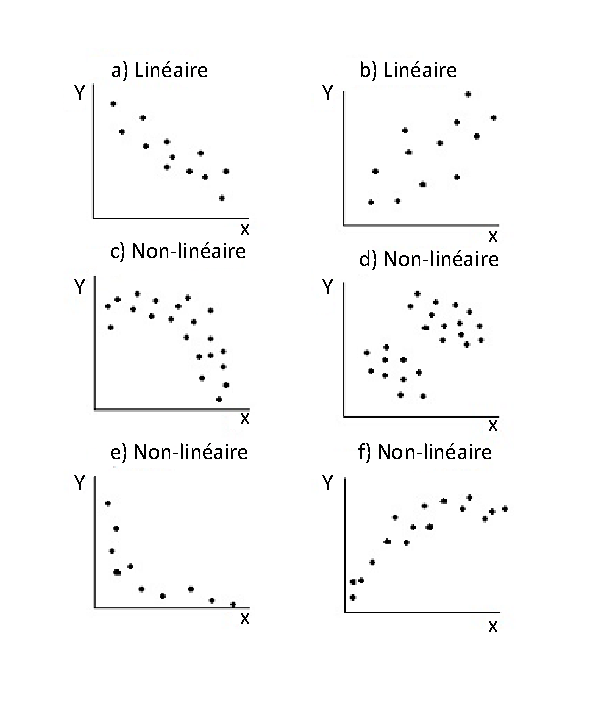
\includegraphics[scale = 1.3]{Chap4-ChoixModeleRLS/Figures/graph_linearite.pdf}
 \caption{Diagramme de dispersion de la variable endogène en fonction de la variable exogène}
 \label{fig:graph_linearite}
\end{figure}

\clearpage

La figure~\ref{fig:graph_linearite_residus} illustre quatre diagrammes de dispersion des résidus en fonction des valeurs prédites. Si le postulat de linéarité est raisonnable, ce graphique devrait montrer un nuage de points centré verticalement en 0. Le nuage de points devrait exhiber une allure complètement aléatoire, c'est-à-dire
qu'il ne devrait exister aucune tendance discernable (par exemple résidus croissants ou décroissants en fonction de $Y_i$, graphique à l'allure quadratique, etc.). Dans cet exemple, seul un diagramme résulte d'une relation linéaire. Les vraies relations desquelles sont issues les données sont indiquées dans le titre des graphiques.

\begin{figure}[htbp]
 \centering
  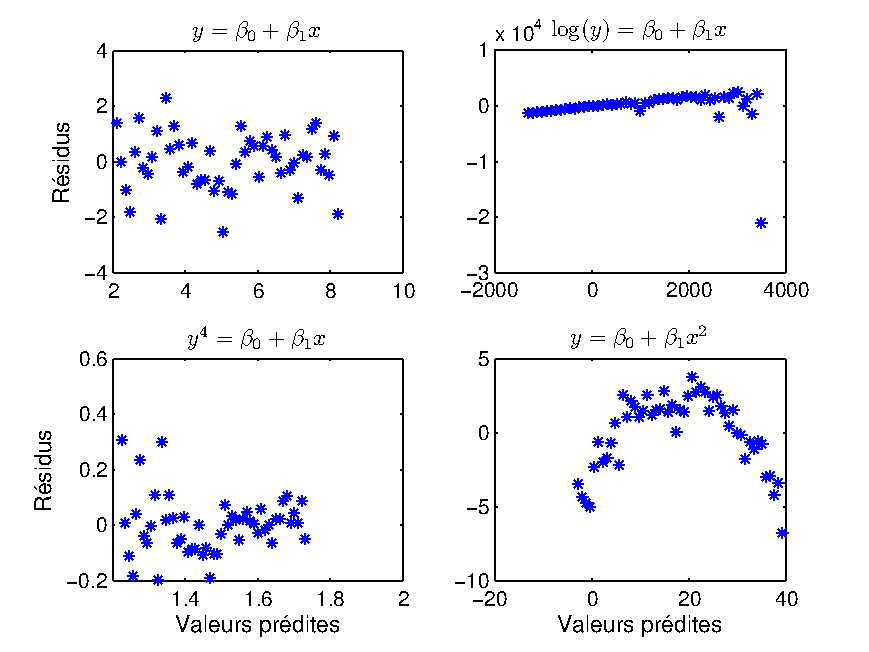
\includegraphics{Chap4-ChoixModeleRLS/Figures/Residus_yhat_Regress_log_ycarre_quadratique.pdf}
 \caption[Exemples de quatre diagrammes de dispersion des résidus en fonction des valeurs prédites.]{Exemples de quatre diagrammes de dispersion des résidus en fonction des valeurs prédites. Dans les quatre cas, le modèle de régression linéaire simple a été ajusté aux données. Le titre de chaque graphique indique le vrai modèle duquel les données sont issues.}
 \label{fig:graph_linearite_residus}
\end{figure}

\clearpage

La figure~\ref{fig:graph_linearite_residus_x} montre quatre diagrammes de dispersion des résidus en fonction de la variable exogène. Comme dans la figure~\ref{fig:graph_linearite_residus}, si le postulat de linéarité est vérifié, ce graphique devrait montrer un nuage de points centré verticalement en 0 et à l'allure aléatoire. À nouveau seul un diagramme est issu d'une relation linéaire. En comparant ces diagrammes en nuages de points avec ceux de la figure~\ref{fig:graph_linearite_residus}, nous constatons que ces deux types de graphiques sont similaires et permettent de tirer les mêmes conclusions.

%\vspace{0.1 in}

\begin{figure}[htbp]
\centering
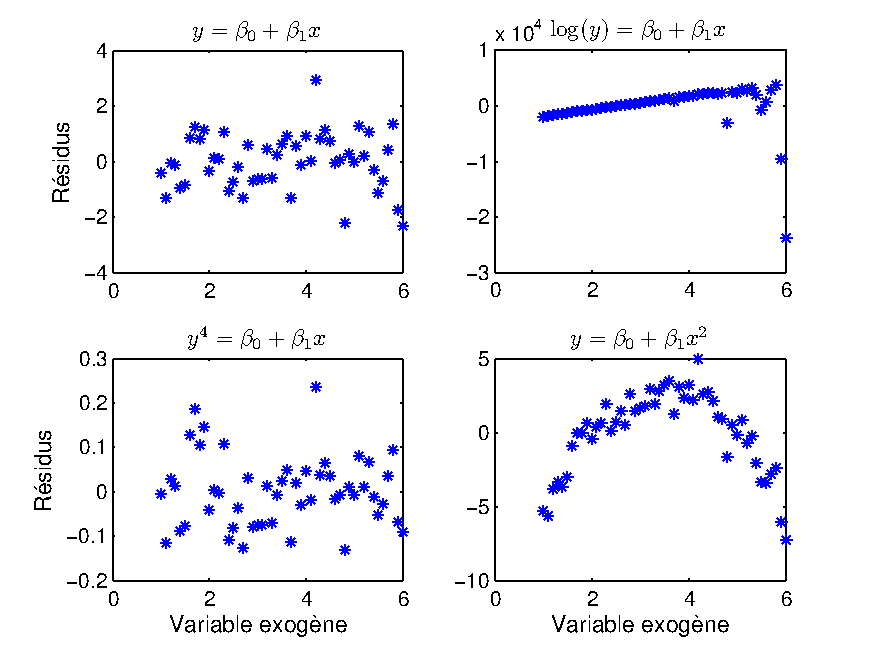
\includegraphics[scale = 0.9]{Chap4-ChoixModeleRLS/Figures/Residus_x_Regress_log_ycarre_quadratique.pdf}
\caption[Exemple de quatre diagrammes de dispersion des résidus en fonction de la variable exogène.]{Exemple de quatre diagrammes de dispersion des résidus en fonction de la variable exogène. Dans les quatre cas, le modèle de régression linéaire simple a été ajusté aux données. Le titre de chaque graphique indique le vrai modèle duquel les données sont issues.}
 \label{fig:graph_linearite_residus_x}
\end{figure}


Il est très important d'examiner les graphiques~\ref{fig:graph_linearite} et \ref{fig:graph_linearite_residus} ou \ref{fig:graph_linearite} et \ref{fig:graph_linearite_residus_x}. Si la relation n'est pas linéaire, la régression linéaire simple ne constitue pas un modèle approprié. Il est alors possible de transformer les données pour obtenir une relation linéaire (voir la \autoref{sec:transfoRLS}). Par exemple, dans le cas d'une relation du type de celles présentées à la figure \ref{fig:graph_linearite} e) et f), on peut tenter un modèle du genre:
 \[1/Y_i = \beta_0 + \beta_1 (1/x_i) + \varepsilon_i
\]
ou
 \[\log(Y_i)= \beta_0 + \beta_1 \log(x_i) + \varepsilon_i.
\]

\begin{remarque}
Les résidus standardisés devraient en général se situer entre -3 et 3, car si le modèle de régression linéaire simple est approprié, ils sont issus d'une distribution normale centrée réduite. On peut vérifier si c'est le cas à l'aide des graphiques utilisés pour tester la linéarité. Si certains résidus possèdent des valeurs plus grandes que 3 en valeur absolue, ceci peut indiquer un manque de normalité, qui sera discuté sous peu, ou la présence de données aberrantes, dont nous reparlerons au \autoref{sec:DonneesInfluentes}.
\end{remarque}


\subsection{Homoscédasticité}
\label{sec:Homoscédasticité}
On a vu que le graphique des résidus standardisés en fonction des valeurs prédites permet de vérifier la linéarité. Le même graphique permet de juger de l'homoscédasticité ($\var[\varepsilon_i]=\sigma^2 \ \ \ 1 \leq i \leq n$). L'hétéroscédasticité signifie que la variance des résidus n'est pas constante. Un graphique pour lequel la variabilité des résidus semble différente pour différentes valeurs des valeurs prédites indique un tel problème. La figure \ref{fig:graphs_homoscedasticite} illustre de façon schématique divers problèmes d'hétéroscédasticité.

\vspace{0.1 in}
\begin{figure}[htbp]
 \centering
  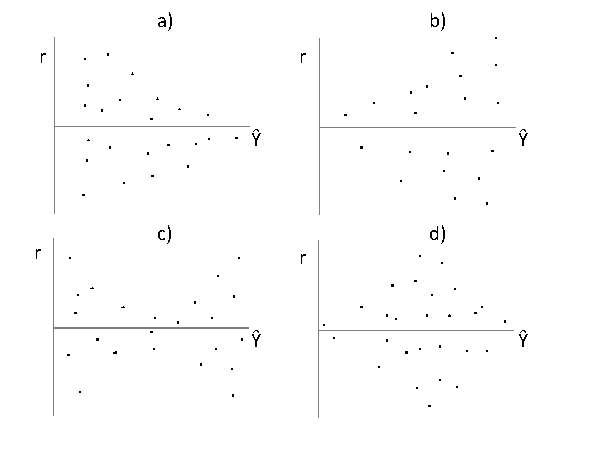
\includegraphics{Chap4-ChoixModeleRLS/Figures/graphs_homoscedasticite}
 \caption{Exemples d'hétéroscédasticité illustrée avec le graphique des résidus standardisés.}
 \label{fig:graphs_homoscedasticite}
\end{figure}

Pour régler le problème d'hétéroscédasticité, on peut également envisager une transformation de la variable endogène.

\newpage
\subsection{Indépendance}
\label{sec:Indépendance}

L'indépendance des observations est plus difficile à tester.

Si les données sont chronologiques, on peut tracer le graphique des résidus en fonction du numéro d'observation. Si aucun patron n'est détecté, le postulat d'indépendance est valable. Sinon, il existe peut-être de l'autocorrélation entre les données (dépendance temporelle). La figure \ref{fig:graphs_autocorrelation} montre un exemple d'autocorrélation positive, et un exemple d'autocorrélation négative. D'autres types de dépendance sont également possibles.


\begin{figure}[h]
\centering
  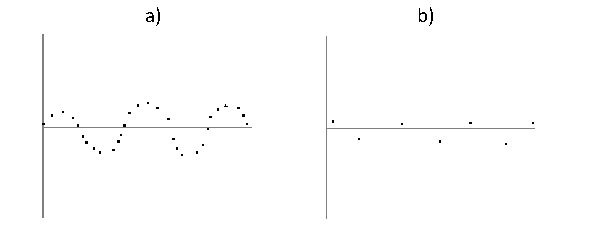
\includegraphics[scale = 1.5]{Chap4-ChoixModeleRLS/Figures/graphs_autocorrelation}
  \caption{Exemple d'autocorrélation positive (a) et négative (b)}
  \label{fig:graphs_autocorrelation}
\end{figure}


Si les données ne sont pas chronologiques, on peut parfois réaliser que $\mathcal{P}_3$ n'est pas valide en analysant la méthode avec laquelle les données ont été collectées. Par exemple, si plusieurs données viennent d'une même unité, il se peut que leurs erreurs soient corrélées.


\subsection{Normalité}
\label{sec:Normalité}


Ce postulat est moins critique que les autres. En effet, même si l'hypothèse de normalité n'est pas vérifiée, $\hat{\beta}_0$, $\hat{\beta}_1$ et $\hat{\sigma}^2$ possèdent un sens dans le cadre du modèle. En revanche, les intervalles de confiance, les tests et les seuils observés sont tous biaisés en l'absence de normalité. Il est possible de vérifier la normalité par des méthodes graphiques (histogramme,  diagramme en boîte (boxplot), droite de Henry) ou par des tests formels (Shapiro-Wilk et Kolmogorov-Smirnov). Dans tous les cas, ces tests sont basés sur les résidus standardisés, car même si ces derniers sont dépendants, ils présentent l'avantage de posséder la même variance.

\subsubsection{L'histogramme}
\label{sec:LHistogramme}

L'histogramme permet de vérifier la symétrie et l'unimodalité. Une distribution normale est unimodale et symétrique, comme illustré à la figure \ref{fig:distresidus}a).

\begin{figure}[htbp]
 \centering
  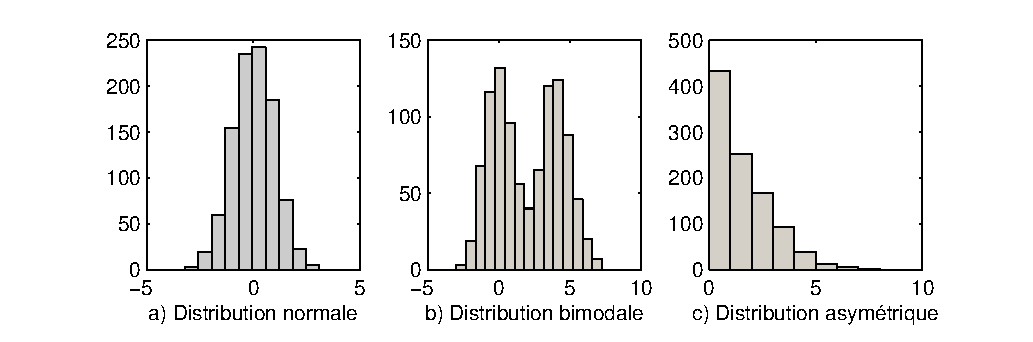
\includegraphics[width=1.00\textwidth]{Chap4-ChoixModeleRLS/Figures/distresidus}
 \caption[Histogramme présentant la distribution des résidus.]{Histogramme présentant la distribution des résidus. Seule la distribution normale (a) est jugée acceptable. Dans les cas b) et c), le modèle apparaît comme n'étant pas adéquat.}
 \label{fig:distresidus}
\end{figure}

\subsubsection{Le diagramme en boîte}
\label{sec:LeDiagrammeÀMoustache}

Le diagramme en boîte, aussi appelé diagramme à moustaches ou \textit{ boxplot} en anglais, permet de vérifier la symétrie, tout comme l'histogramme. Il permet aussi d'identifier la présence de valeurs extrêmes. Une valeur est considérée comme extrême (et indiquée par un symbole particulier) si elle est à l'extérieur des bornes $$\hat q(25\%)-1,5 \times \left\{\hat q(75\%)-\hat q(25\%)\right\} \mbox{   ,    } \hat q(75\%)+1,5 \times \left\{\hat q(75\%)-\hat q(25\%)\right\}$$ où $\hat{q}(\cdot)$ désigne le quantile empirique. Trop de valeurs extrêmes indiquent un problème de normalité, un problème potentiel lors de l'échantillonnage, un problème de linéarité ou alors la présence de deux populations distinctes.

 La figure \ref{fig:boxplot_residus} montre trois diagrammes en boîte des résidus. Le diagramme de gauche est typique d'une distribution normale, celui du centre illustre la présence de valeurs extrêmes indiquées par le symbole $+$, alors que le diagramme de droite reflète une asymétrie des résidus.

\newpage

\begin{figure}[htbp]
 \centering
  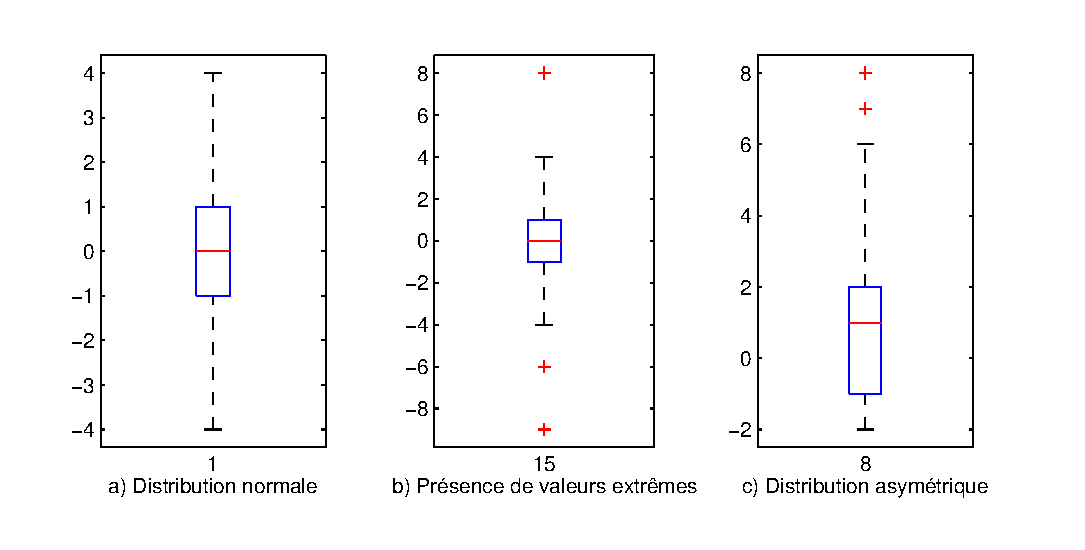
\includegraphics[scale = 0.7]{Chap4-ChoixModeleRLS/Figures/boxplot_residus.eps}
 \caption{Exemple de diagrammes en boîte représentant les résidus.}
 \label{fig:boxplot_residus}
\end{figure}


\subsubsection{Le diagramme quantile-quantile normal}
\label{sec:LaDroiteDeHenry}


L'idée de base ici est que si un échantillon suit une certaine loi, les quantiles empiriques observés dans les données devraient être similaires aux quantiles théoriques de cette loi. Ainsi,  un graphique des quantiles empiriques versus les quantiles théoriques devrait ressembler à une droite de pente 1 passant par l'origine.

On nomme diagramme quantile-quantile normal (\textit{normal QQ-plot}) le nuage de points qui illustre les quantiles empiriques en fonction des quantiles théoriques. Puisqu'on souhaite tester la normalité des résidus, on utilise les $n$ quantiles théoriques de la loi normale centrée réduite, qu'on compare aux quantiles empiriques des résidus standardisés $r_i$.

Un deuxième type de graphique très similaire compare plutôt les statistiques d'ordre théoriques avec les valeurs observées. On le nomme habituellement droite de Henry.\footnote{Le terme droite de Henry est parfois utilisé aussi pour un QQ-plot qui teste la normalité.} Voici concrètement comment le construire:

\begin{enumerate}
 \item On ordonne les résidus standardisés $r_{i}$, qu'on note $r_{(i)}$.
 \item On calcule l'espérance des statistiques d'ordre de la loi normale centrée réduite donnée par $$u_{(i)}=\esp[Z_{(i)}]=\int_{-\infty}^{\infty}zn{n-1 \choose i-1}\Phi^{i-1}(z)\varphi(z)dz$$ où $\varphi(z)=\frac{1}{\sqrt{2\pi}}\exp(-z^2/2)$ et $\Phi(z)=\int_{-\infty}^z\varphi(t)dt$. Lorsque $n$ est grand, il est possible d'utiliser l'approximation suivante $\esp[Z_{(i)}]= \Phi^{-1} \left(\frac{i-3/8}{n-1/4}\right)$.
 \item On trace le graphique de $r_{(i)}$ en fonction de $u_{(i)}$
\end{enumerate}

Si les résidus sont normaux, les points devraient être alignés. Lorsque les points forment une courbe concave ou convexe, la distribution des résidus est non
symétrique. Un graphique en forme de S  indique un aplatissement différent de la
 distribution  normale. La figure \ref{fig:qqplot_residus} montre des exemples de droites de Henry. Le graphique a) illustre le cas d'une distribution normale alors que les deux autres graphiques indiquent respectivement des queues trop lourdes (b) et trop légères (c).
\begin{figure}[htbp]
 \centering
  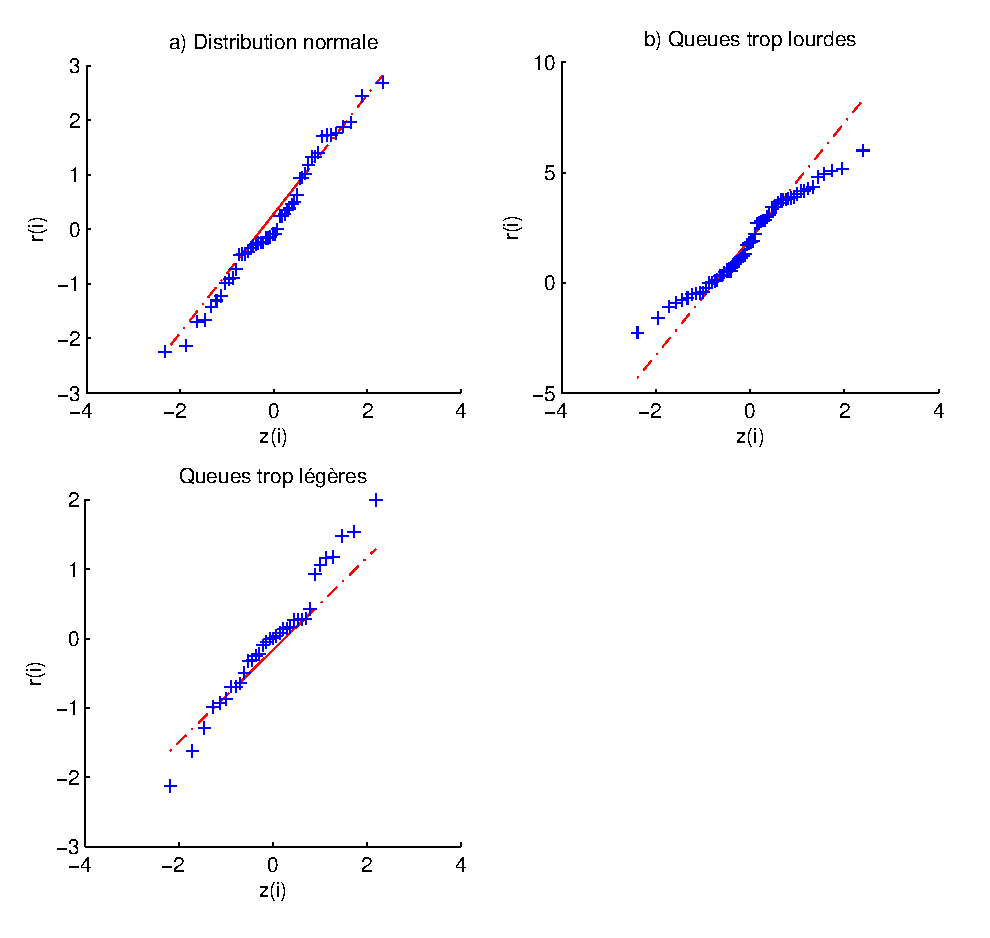
\includegraphics[scale = 0.7]{Chap4-ChoixModeleRLS/Figures/qqplot_residus.eps}
 \caption{Droites de Henry }
 \label{fig:qqplot_residus}
\end{figure}


\vspace{-0.1in}
\subsubsection{Tests formels}

Les graphiques suffisent fréquemment pour confirmer ou infirmer les postulats du modèle. Cependant il n'est pas rare que l'interprétation de certains graphiques soit difficile et puisse paraître ambiguë. Dans ces cas, il existe certains tests d'hypothèses formels permettant de vérifier les postulats. La possibilité de faire un test formel ne signifie toutefois pas qu'il faille négliger les approches graphiques, car ces dernières permettent d'identifier ce qui crée la non-normalité (asymétrie, valeurs extrêmes), ce que les tests formels ne permettent pas de faire.


\newpage
Nous présentons ici deux tests de normalité. Les hypothèses dans les deux cas sont
\begin{align*}
H_0: & \mbox{ Les erreurs sont distribuées selon une loi normale.}\\
H_1: & \mbox{ Le postulat de normalité des erreurs n'est pas vérifié.}
\end{align*}
De grandes valeurs de $p$ indiqueront donc que l'hypothèse de normalité est respectée.

\textbf{Test de Shapiro-Wilk}

La statistique du test de Shapiro-Wilk est la suivante:
\begin{align*}
 W= \frac{\left(\sum_{i=1}^n a_i r_{(i)} \right)^2}{\sum_{i=1}^n (r_i-\overline{r})^2} & \hspace{2cm} \mbox{où} & a_i &= \frac{\overline{Z}^T V^{-1}}{\sqrt{\overline{Z}^T V^{-1}\overline{Z}}}\\
 & &\overline{Z} &= (\esp[Z_{(1)}],...,\esp[Z_{(n)}])
\end{align*}
Ici, $Z_{(i)}$ est la $i^e$ statistique d'ordre d'une loi normale centrée réduite, $V$ est la matrice de variance-covariance des $Z_{(i)}$, et $\overline r=0$.

La statistique $W$ est à peu près équivalente à un coefficient de détermination entre les variables $r_{(i)}$ et $u_{(i)} = \esp(Z_{(i)})$. On peut ainsi faire le lien entre la droite de Henry et la statistique de Shapiro-Wilk. En effet une valeur de $W$ proche de 1 indique un bon alignement des points sur la droite de Henry. L'avantage du test de Shapiro-Wilk est qu'il permet de faire un test formel basé sur la distribution de $W$ sous l'hypothèse nulle que $W=1$. Les logiciels fournissent une $p$-valeur pour ce test.

\textbf{Le test de Kolmogorov-Smirnov}

De façon générale, le test de Kolmogorov-Smirnov permet de tester si un échantillon suit une loi quelconque, de répartition $F$. Ce test est basé sur la distance entre cette loi  sous $H_0$ (notée $F_0$) et l'estimation non paramétrique de $F$, c'est-à-dire la fonction de répartition expérimentale
 \[ F_n (x)=\frac{1}{n} \sum_{i=1}^n \I (x_i \leq x) \ \ \ \ \ \ \ x\in \R.
\]

Lorsque $n \rightarrow \infty$, $ F_n (x) \rightarrow F_0 (x)$. Dans le cadre de la régression, on souhaite tester si l'échantillon suit une loi normale. L'hypothèse nulle du test est donc $H_0: F_0$ est la distribution normale. La statistique du test est:
\begin{eqnarray*}
 D_n = \sup_{x} \left|F_n (x) - F_0 (x) \right|
\end{eqnarray*}

Si l'hypothèse nulle est vraie, alors $D_n$ est proche de 0. Les logiciels fournissent une $p$-valeur pour le test de Kolmogorov-Smirnov. Bien que très utilisé, ce test est peu puissant et on lui préfère le test de Shapiro-Wilk.


\subsection{Exemple}

Les données de la section \ref{exemple-RLS-interpretation} ne sont pas très intéressantes pour vérifier la validité des postulats étant donné que la relation linéaire est presque parfaite. On s'intéressera plutôt ici à la concentration d'ozone dans l'atmosphère.

La pollution de l'air constitue une préoccupation majeure de santé publique. De nombreuses recherches ont démontré l'influence sur la santé de certains composés chimiques tels l'ozone (O$_3$). Certaines catégories de la population, tels les nouveaux-nés, les personnes âgées et les personnes asthmatiques, sont particulièrement sensibles à la pollution. La prévision des pics de concentration des polluants revêt par conséquent une grande importance.

Les lois de la chimie nous informent que cette concentration augmente avec la température. L'association de la surveillance de la qualité de l'air en Bretagne (nommée \texttt{Air Breizh}) mesure depuis plusieurs années la concentration en ozone toutes les 10 minutes ainsi que des données météorologiques comme la température et le vent à certaines heures de la journée.  L'objectif de cet exemple consiste à prédire le maximum journalier de concentration d'ozone en fonction de la température à 12h. Pour cela on se base sur un échantillon de 112 observations mesurées du 1er juin au 30 septembre 2001 par \texttt{Air Breizh}. Pour plus de détails concernant la base de données, le lecteur se référera à  \citet[][Section 1.1.1]{Cor_Mat:07}.
%Les données sont disponibles sur le site web de Pierre-André Cornillon à l'adresse \url{http://www2.agrocampus-ouest.fr/math/livreR/ozone.txt}. Inactif

On choisit comme modèle la régression linéaire simple. La variable endogène est la concentration maximale d'ozone mesurée dans une journée, en $\mu$g/ml (maxO3). La température à 12h (T12) constitue la variable exogène. Le modèle s'exprime donc:
\begin{eqnarray*}
  \max \mbox{O}3 &=& \beta_0 + \beta_1 \mbox{T}12 +\varepsilon.
\end{eqnarray*}
On peut calculer que $\hat{\beta_0} = -27,42$ et que $\hat{\beta_1} = 4,65$.

%Les postulats du modèle comprennent : 1) la linéarité de la relation, 2) l'homoscédasticité, 3) l'indépendance et 4) la normalité des résidus.
%Comme l'objectif est une prévision, le postulat de normalité doit être respecté.

Regardons maintenant la validité des postulats. La figure \ref{fig:ozone_FitPlot1} permet de supposer que la linéarité est respectée. Il en va de même pour le graphique des résidus studentisés (figure \ref{fig:ozone_RStudentByPredicted1}). Ce dernier graphique permet en outre de constater que la variance des résidus est constante. Le postulat d'homoscédasticité est donc lui aussi respecté.


\begin{figure}
  \centering
  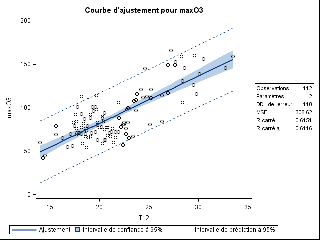
\includegraphics[width=12cm]{Chap4-ChoixModeleRLS/Figures/ozone/FitPlot1.pdf}\\
  \caption[Droite de régression de l'ozone en fonction de la température]{Droite de régression de l'ozone en fonction de la température. Ici, la linéarité ne semble pas causer de problème. Notez que le graphique montre également la droite de régression, l'intervalle de confiance à 95\% (en ombragé bleu) et l'intervalle de prévision (en pointillé).}\label{fig:ozone_FitPlot1}
\end{figure}
\begin{figure}
  \centering
  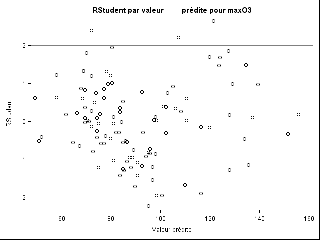
\includegraphics[scale = 2]{Chap4-ChoixModeleRLS/Figures/ozone/RStudentByPredicted1.pdf}\\
  \caption[Graphique des résidus studentisés pour l'exemple de l'ozone]{Graphique des résidus studentisés pour l'exemple de l'ozone. Ce graphique permet de constater que la relation est linéaire et que la variance des résidus est constante.}\label{fig:ozone_RStudentByPredicted1}
\end{figure}

\clearpage

Puisque les données sur l'ozone et la température sont collectées à différents moments, il s'agit d'une série temporelle et il y a un potentiel d'autocorrélation. Le graphique des observations en fonction du numéro d'observation (figure \ref{fig:ozone_independance}) permet en effet de douter de l'indépendance des observations. Ce type de problème est fréquent lorsque l'on travaille avec des données temporelles. Il faudrait dans ce cas faire des tests formels d'autocorrélation. Toutefois, puisque ces tests ne font pas l'objet de ce cours et que les patrons observés sont tout de même vagues, on considérera en pratique que le postulat d'indépendance est respecté.


\begin{figure}[h!]
  \centering
  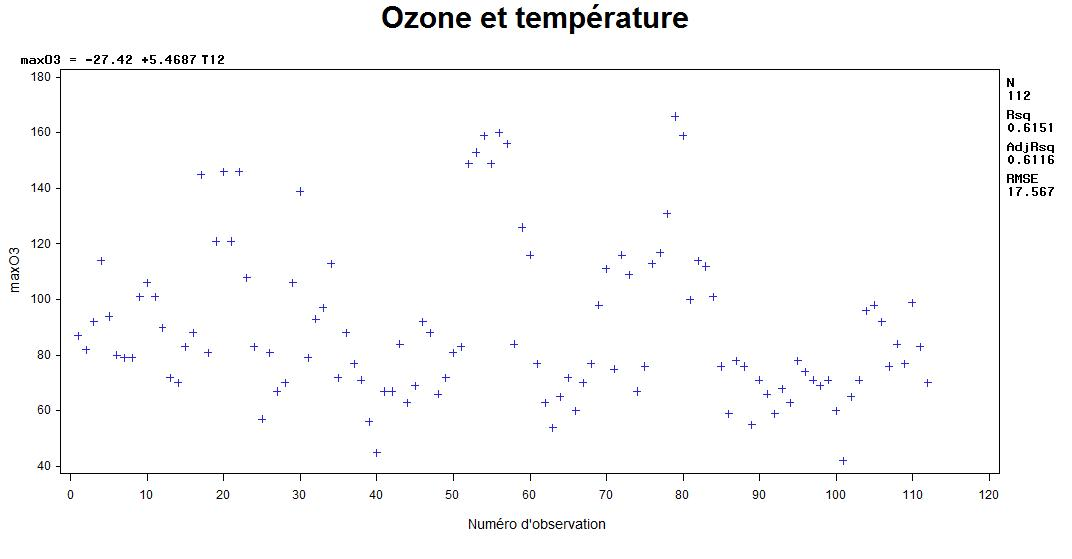
\includegraphics[width=15cm]{Chap4-ChoixModeleRLS/Figures/ozone/independance.jpg}\\
  \caption{Vérification de l'indépendance des observations. On observe quelques vagues patrons qui pourraient signifier qu'il y a autocorrélation.}\label{fig:ozone_independance}
\end{figure}


En ce qui concerne le postulat de normalité, les méthodes graphiques suggèrent toutes que les résidus sont normaux (voir les figures \ref{fig:ozone_ResidualHistogram1}, \ref{fig:ozone_ResidualBoxPlot1} et \ref{fig:ozone_QQPlot1}). Les tests formels confirment le respect du postulat de normalité (tableau \ref{tab:ozone_test_normalite}). La statistique de Shapiro-Wilk est de 0,99. Cette statistique peut être interprétée comme étant le $R^2$ de la droite de Henry. La statistique de Shapiro-Wilk et la figure \ref{fig:ozone_QQPlot1} sont donc cohérentes. L'hypothèse nulle du test de Shapiro-Wilk est que les résidus sont normaux. Avec une $p$-valeur de 0,79, on ne peut pas rejeter cette hypothèse. Quant au test de Kolmogorov-Smirnov, dont l'hypothèse nulle est aussi la normalité des résidus, sa $p$-valeur est supérieure à 0,15. Les deux tests aboutissent donc à la même conclusion: les résidus suivent une distribution normale.

Toutes les hypothèses de la régression linéaire simple sont donc satisfaites pour ce jeu de données.

\newpage

\begin{figure}
\centering
\begin{minipage}{.45\textwidth}
  \centering
  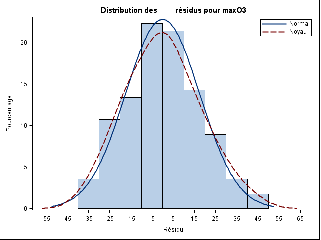
\includegraphics[scale = 1.3]{Chap4-ChoixModeleRLS/Figures/ozone/ResidualHistogram1.pdf}\\
  \captionof{figure}{Histogramme des résidus. La forme de l'histogramme est typique d'une distribution normale.}
  \label{fig:ozone_ResidualHistogram1}
\end{minipage}%
\hspace{1 cm}
\begin{minipage}{.45\textwidth}
  \centering
  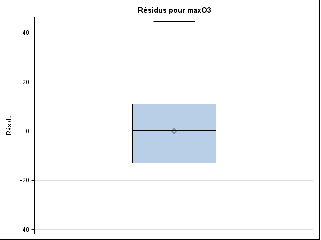
\includegraphics[scale = 1.3]{Chap4-ChoixModeleRLS/Figures/ozone/ResidualBoxPlot1.pdf}\\
  \captionof{figure}{Diagramme en boîte des résidus. Les résidus sont à peu près symétriques et on n'observe aucune valeur extrême.}
  \label{fig:ozone_ResidualBoxPlot1}
\end{minipage}
\end{figure}


\begin{figure}
\centering
  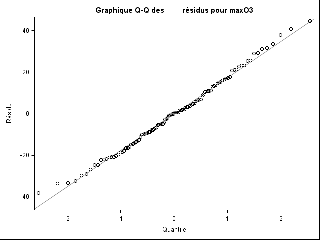
\includegraphics[scale = 1.3]{Chap4-ChoixModeleRLS/Figures/ozone/QQPlot1.pdf}\\
  \caption[Droite de Henry]{Droite de Henry. Les points sont très bien alignés sur la droite; la distribution des résidus semble normale.}
  \label{fig:ozone_QQPlot1}
\end{figure}

\begin{figure}
  \centering
  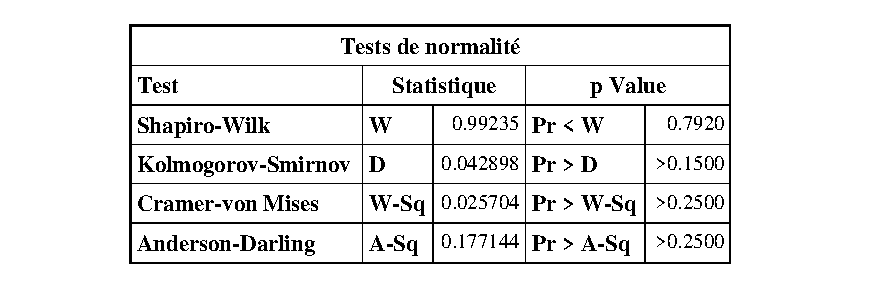
\includegraphics[scale = 0.8]{Chap4-ChoixModeleRLS/Figures/ozone/test_normalite.pdf}\\
  \caption{Résultat des tests de normalité.}
\label{tab:ozone_test_normalite}
\end{figure}

\clearpage

\section{Transformation des données}
\label{sec:transfoRLS}

Si les postulats de la régression ne sont pas respectés, et donc que le modèle \\$y_i~=~\beta_0 ~+~ \beta_1 ~x_i ~+ ~\varepsilon_i$ ne colle pas à la réalité, on peut effectuer une transformation des variables qui permettra d'utiliser le modèle de régression linéaire.  Il existe en effet souvent une fonction $g(\cdot)$ qui transforme une des variables de façon à régler un problème de linéarité, d'hétéroscédasticité ou de normalité. On propose ici trois méthodes pour trouver $g(\cdot)$.



\subsection{La technique de Mosteller et Tukey}
\label{sec:LaTechniqueDeMostellerEtTukey}


La technique de Mosteller et Tukey est une méthode graphique généralement utilisée pour régler un problème de linéarité, mais qui peut aussi être utile dans le cas d'un problème de normalité. On trace simplement le graphique de la variable endogène en fonction de la variable exogène et on observe la forme du nuage de points. %trouver une fonction $g(\cdot)$ appropriée à l'aide des diagrammes de dispersion des couples $[x_i; g(Y_i)]$ pour plusieurs choix de $g(\cdot)$, jusqu'à obtention d'un graphique d'apparence le plus linéaire possible.
La \autoref{fig:Mosteller_Tukey} montre quel type de transformation est appropriée à chaque forme de nuage de points.

\begin{figure}[htb]
 \centering
  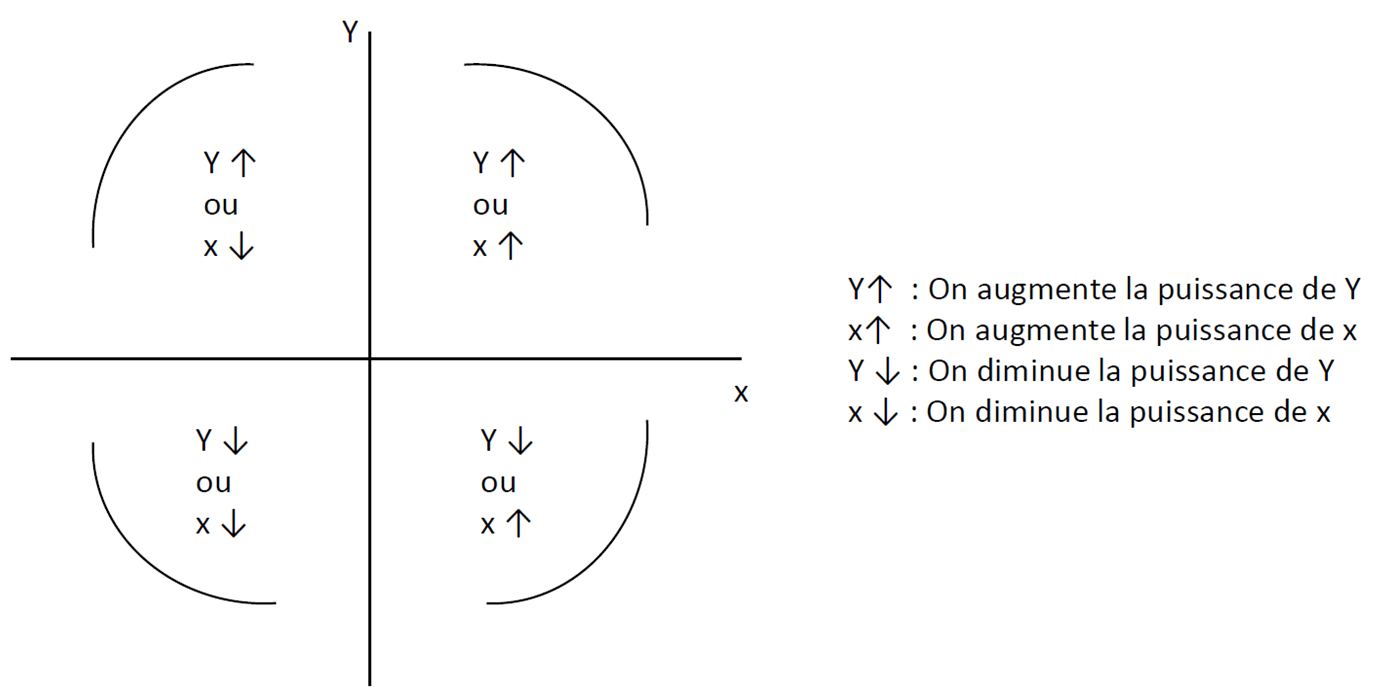
\includegraphics[scale = 0.6]{Chap4-ChoixModeleRLS/Figures/Mosteller_Tukey_2}
 \caption{Transformation des variables avec la technique de Mosteller-Tukey}
 \label{fig:Mosteller_Tukey}
\end{figure}

En pratique, on peut tester plusieurs transformations possibles de la variable endogène et/ou de la variable exogène, telles que suggérées par la méthode. On choisira le modèle pour lequel les hypothèses de la régression linéaire simple semblent le plus valides.

\begin{remarque}
Il vaut mieux si possible appliquer la transformation à la variable exogène plutôt qu'à la variable endogène. La prévision à l'aide du modèle et l'interprétation des intervalles de confiance et de prévision seront plus faciles. Voir section \ref{subsection:previsiontrans}.
\end{remarque}

\subsection{La technique de Box-Cox}
\label{sec:LaTechniqueDeBoxCox}


L'idée de Georges Box et David Cox, publiée en 1964, consiste à généraliser le modèle de régression en introduisant un paramètre supplémentaire $\lambda$ dans le modèle. Plus précisément, on considère le modèle
\begin{eqnarray}
 g(Y_i,\lambda)=\beta_0 + \beta_1 x_i + \varepsilon_i
 \label{eq:reg_box_cox}
\end{eqnarray}
où
\begin{equation}\label{eq:gboxcox}
g(y;\lambda)=\left\{\begin{array}{ll}{y^\lambda-1\over\lambda}, & \lambda\neq0\\
\log(y), & \lambda=0.\end{array}\right.
\end{equation}
et $\lambda$ est un paramètre inconnu à estimer à partir des données.


On suppose la normalité des termes d'erreurs\footnote{La technique peut être contestée du fait de cette hypothèse} et on maximise la vraisemblance par rapport à $\beta_0 , \beta_1, \sigma^2$ et $\lambda$.
Pour cela on pose $W_i(\lambda)=\beta_0+\beta_1 x_i+\varepsilon_i$. Comme on a supposé la normalité des termes d'erreur, on a que $W_i\sim\N(\beta_0+\beta_1 x_i,\sigma^2)$. La vraisemblance s'exprime alors comme
\begin{eqnarray*}
L(\beta_0,\beta_1,\sigma,\lambda)=\prod_{i=1}^n f(W_i)=\prod_{i=1}^n \left(\frac{1}{\sqrt{2\pi\sigma^2}}\right)\exp\left[-\frac{1}{2}\left\{\frac{W_i-(\beta_0+\beta_1 x_i)}{\sigma}\right\}^2\right]J(\lambda),
\end{eqnarray*}
où $J(\lambda)$ note le jacobien de la transformation.

Le problème qui se pose à ce point est que l'on ne peut résoudre $$\frac{\partial L}{\partial \beta_0}=\frac{\partial L}{\partial \beta_1}=\frac{\partial L}{\partial \sigma^2}=\frac{\partial L}{\partial \lambda}=0$$ explicitement. La plupart des logiciels ont des routines pour estimer $\lambda$ numériquement et donnent également un intervalle de confiance pour la valeur de $\lambda$.

Une fois qu'on a estimé $\lambda$, l'\autoref{eq:gboxcox} indique la transformation à utiliser. En pratique, on effectue simplement la régression de $y^{\hat{\lambda}}$ en fonction de $x$.

Si $\lambda = 0$, alors on utilise $\log(Y)$. En effet, $\displaystyle\lim_{\lambda\rightarrow 0}\frac{y^\lambda-1}{\lambda}=\displaystyle\lim_{\lambda\rightarrow 0}\frac{y^\lambda\log(y)}{1}=\log(y).$ Si l'intervalle de confiance de $\lambda$ contient $0$ une transformation logarithmique peut donc être appropriée.

\begin{remarque}
On doit aussi considérer l'interprétation du modèle dans le choix des transformations. Ainsi, une variable à la puissance $1,8765$ est souvent plus difficile à concevoir et à interpréter qu'une variable à la puissance 2. On préférera donc généralement arrondir les puissances.
\end{remarque}

\subsection{Technique de stabilisation de la variance}
\label{sec:Approx_var}

Cette méthode est utilisée en cas de problème d'hétéroscédasticité. Dans ce cas, il y a un lien entre la variation des résidus et les valeurs ajustées. On peut donc dire que la variance des résidus est une fonction de l'espérance de la valeur de $Y$. L'idée est de choisir une transformation $g()$ de sorte que $g(y)$ ait une variance constante.

Le choix des transformations possibles pour stabiliser la variance se base sur la formule approximative pour la variance d'une variable transformée $g(Y)$. Le développement de Taylor du premier ordre conduit à
\begin{eqnarray*}
g(Y)& = & g(\esp[Y]+\{Y-\esp[Y]\}) \\
& \approx  & g(\esp[Y])+g'(\esp[Y])(Y-\esp[Y]).
\end{eqnarray*}
La variance peut donc être approchée par
\begin{eqnarray}
\var[g(Y)]\approx \left\{g'(\esp[Y])\right\}^2\var[Y].
 \end{eqnarray}
 Soit par exemple $Y$ une variable aléatoire telle que son écart-type en fonction de l'espérance est $\sigma(\mu)=\mu^{1/2}$. La substitution dans la formule aproximative pour la variance nous montre que  $\var[g(Y)]\approx \{g'(\mu)\}^2\sigma^2=\{g'(\mu)\}^2\mu.$ La transformation $g(\cdot)$ telle que la variance de $g(Y)$ soit constante doit donc vérifier $g'(\mu)$ proportionnelle à $1/\sqrt{\mu}$, c'est-à-dire $g(Y)=\sqrt Y$ à une constante près.

Lorsque $Y$ prend des valeurs positives, les transformations les plus utiles sont résumées dans le tableau \ref{tab:TransformationHeteroscedasticite}.

{\small
\begin{table}[htbp]
 \centering
 \caption{Transformations envisageables pour régler l'hétéroscédasticité}
  \renewcommand{\arraystretch}{1.6}
  \begin{tabular}{cc}
   \hline
   Transformation typique & Situation \\
   \hline
   $\sqrt{Y}$  & $\var[\varepsilon_i] \propto \esp[Y_i]$ \\
    & (données de type Poisson) \\ \hline
   $\log (Y)$ & $\var[\varepsilon_i] \propto (\esp[Y_i])^2$  \\
   &  (efficace si $Y$ possède une très grande étendue)\\ \hline
   $1/Y$  & $\var[\varepsilon_i] \propto (\esp[Y_i])^4$\\ \hline
   $\arcsin(\sqrt{Y})$ & $Y\in [0,1]$ et $\var[\varepsilon_i] \propto \esp[Y_i] (1-\esp[Y_i])$\\
   & ($Y$ suit une loi Bernoulli)\\
  \end{tabular}
 \label{tab:TransformationHeteroscedasticite}
\end{table}
}



\subsection{Prévision sous transformation}
\label{subsection:previsiontrans}

Il faut être prudent lorsqu'on applique une transformation à la variable endogène. En effet les prévisions sont alors obtenues en termes de la variable endogène transformée. Or, en général on a que,
$$ \esp[g(Y)]\neq g(\esp[Y]).$$ Il est donc incorrect de simplement appliquer la transformation inverse afin d'obtenir une prévision en termes de la variable aléatoire endogène $Y$ de base (non transformée).

La détermination d'un intervalle de confiance est par contre directe, en utilisant le fait que lorsque $g(\cdot)$ est une fonction monotone, on a que
$$\P\{a\leq g(Y)\leq b\}=\P\{g^{-1}(a)\leq Y\leq g^{-1}(b)\},$$ où $g^{-1}$ désigne la transformation inverse.

%\textcolor{red}{Ajouter quelque chose sur la transformation?}

\begin{exemple}
Soit le modèle de régression linéaire simple suivant :
$$\sqrt{Y}=Y_i^*=\beta_0+\beta_1 x_i+\varepsilon_i.$$ Un intervalle de confiance à 90 \% pour $g(Y)$ lorsque $x=x_0$ est donné par $(0,2;2,4)$. On désire trouver un intervalle de prévision à 90 \% pour $Y$ lorsque $x=x_0$. \\
On a que $Y^*=\sqrt{Y}\Leftrightarrow Y=(Y^{*})^2$.\\
L'intervalle de prévision en termes de la variable endogène de base $Y$ sera donc
$$((0,2)^2;(2,4)^2)=(0,04;5,76).$$
%On ne peut toutefois pas obtenir aisément de prévision pour $Y_i$.
\end{exemple}



\chapter{Ajuster un modèle de régression linéaire multiple (RLM)}
\label{sec:AjusterRLM}

% À voir la pertinence de cette section
\vspace{-0.1in}
\section{Préambule : notation matricielle de la RLS}

Le traitement de la régression linéaire peut être grandement approfondi
en utilisant la notation matricielle et les résultats de l'algèbre linéaire. On considère d'abord la notation matricielle dans le cas de la régression linéaire simple, i.e. avec une seule variable explicative.

Soient $\boY$, le vecteur de dimension $(n\times 1)$ des observations de la variable endogène, $\boX$ la matrice de dimension $(n\times 2)$ des valeurs de la variable exogène, $\bobeta$ le vecteur de dimension $(2\times 1)$ des coefficients de régression et $\boeps$ le vecteur de dimension $(n \times 1)$ des termes d'erreurs:
$$
\boY=\underbrace{\left(\begin{array}{c} Y_1\\ Y_2\\ \vdots\\ Y_n\end{array}\right)}_{n\times 1}
\ \ \ \bobeta=\underbrace{\left({\beta_0\atop\beta_1}\right)}_{2 \times 1}\ \ \
\boX=\underbrace{\left(\begin{array}{cc} 1 & x_1\\ 1 & x_2\\ \vdots & \vdots \\
1 & x_n\end{array}\right)}_{n\times 2}\ \ \
\boeps=\underbrace{\left(\begin{array}{c}\varepsilon_1\\ \varepsilon_2\\ \vdots\\
\varepsilon_n\end{array}\right)}_{n\times 1}.
$$
On a que
$$\underbrace{\left(\begin{array}{c} Y_1\\ Y_2\\ \vdots\\ Y_n\end{array}\right)}_{n\times 1}=\underbrace{\left(\begin{array}{cc} 1 & x_1\\ 1 & x_2\\ \vdots & \vdots \\
1 & x_n\end{array}\right)}_{n\times 2} \underbrace{\left({\beta_0\atop\beta_1}\right)}_{2 \times 1}+\underbrace{\left(\begin{array}{c}\varepsilon_1\\ \varepsilon_2\\ \vdots\\
\varepsilon_n\end{array}\right)}_{n\times 1}
$$
En utilisant ces notations, le modèle de régression linéaire simple défini à l'équation \eqref{eq:reg_lin_simple} peut s'exprimer ainsi :
\begin{equation}\label{eq:rlsmat}
\boY=\boX\bobeta+\boeps.
\end{equation}

	

\section{Le modèle de régression linéaire multiple}
\label{sec:ModèleEtNotation}
Le modèle de régression linéaire multiple constitue une généralisation du modèle de régression linéaire simple qui permet de mettre en relation une variable endogène notée $Y$ avec plusieurs variables exogènes notées $(x_1, x_2, ..., x_p$). L'équation du modèle de régression linéaire multiple s'exprime de la manière suivante
\begin{eqnarray}
	Y_i = \beta_0 + \beta_1 x_{i1} +  \beta_2 x_{i2}+ \ldots + \beta_p x_{ip} + \varepsilon_i, \;\;\;\;\;\; i=1,\ldots,n;\;\;\; j=1,\ldots,p
\label{eq:reg_lin_mult}
\end{eqnarray}
\vspace{-0.05in}
où
\begin{itemize}
\item[$\bullet$] $Y_i, i=1\ldots,n$, représente la variable endogène pour l'observation $i$
\item[$\bullet$] $x_{ij}$ est la valeur de la j-ème variable pour l'observation $i$
%Il est possible de multiplier la variable $\beta_0$ par $x_{i0}=1, i=1\ldots,n$. Dans ce cas, $\beta_0$ représente la constante, appelée également \textit{intercept} en anglais.
\item[$\bullet$] $\beta_0$ et $\beta_j, j=1,\dots,p$ sont les paramètres du modèle
% qui sont inconnus et par conséquent doivent être estimés.
\item[$\bullet$] $\varepsilon_i$ représente le terme d'erreur pour l'observation $i$.\\
\end{itemize}

Dans sa version matricielle, le modèle s'écrit comme suit:

\[ \underbrace{\left(
\begin{MAT}(r)[2pt,0pt,3cm]{c}
Y_1 \\
Y_2 \\
\vdots \\
Y_n \\
\end{MAT}
\right)}_{n\times 1} = \underbrace{\left(
\begin{MAT}(r)[2pt,0pt,3cm]{ccccc}
1 & x_{11} & x_{12} & \cdots & x_{1p} \\
1 & x_{21} & x_{22} & \cdots & x_{2p} \\
\vdots & \vdots & \vdots &\ddots &\vdots \\
1 & x_{n1} & x_{n2} & \cdots & x_{np}\\
\end{MAT}
\right)}_{n\times (p+1)}  \underbrace{\left(
\begin{MAT}(r)[2pt,0pt,3cm]{c}
\beta_0\\
\beta_1 \\
\vdots\\
\beta_p\\
\end{MAT}
\right) }_{(p+1)\times 1}+ \underbrace{\left(
\begin{MAT}(r)[2pt,0pt,3cm]{c}
\varepsilon_1\\
\varepsilon_2 \\
\vdots\\
\varepsilon_n\\
\end{MAT}
\right)}_{n\times 1}
\]
soit
\vspace{-0.05in}
\begin{eqnarray}
	\boY_{n\times 1} = \boX_{n\times p'} \bobeta_{p'\times 1} + \boeps_{n\times 1}
\label{eq:reg_lin_mult_mat}
\end{eqnarray}
\vspace{-0.05in}
où
\begin{itemize}
\item[$\bullet$]$\boY$ désigne le vecteur contenant la variable endogène (dimension $n \times 1$)
\item[$\bullet$] $\boX$ note la matrice d'incidence contenant les variables exogènes (dimension $n \times p'$)
\item[$\bullet$] $\bobeta$ est le vecteur des coefficients de la régression (dimension $p' \times 1$)
\item[$\bullet$] $\boeps$ dénote le vecteur des termes d'erreur (dimension $n\times 1$)
\item[$\bullet$] $n$ note le nombre d'observations
\item[$\bullet$] $p$ indique le nombre de variables exogènes
\item[$\bullet$] $p'=p+1$ désigne le nombre de paramètres à estimer
%(un coefficient par variable + l'ordonnée à l'origine).
\end{itemize}


\subsection{Postulats du modèle de RLM}
\label{sec:PostulatsRLM}

Les quatre postulats du modèle de régression linéaire multiple sont similaires à ceux de la régression linéaire simple, à savoir :
\begin{itemize}
\item [$\mathcal{P}_1.$] $\esp[\varepsilon_i]=0$, pour $i=1,\ldots,n$.
\item [$\mathcal{P}_2.$] $\var[\varepsilon_i]=\sigma^2$, pour $i=1,\ldots,n$.
\item [$\mathcal{P}_3.$] $\cov[\varepsilon_i,\varepsilon_j]=0$ pour $i\neq j$.
\item [$\mathcal{P}_4.$] $\varepsilon_i$ est distribué selon une loi normale pour $i=1,\ldots,n$.
\end{itemize}

\subsection{Interprétation des paramètres}
\label{sec:InterpétationRLM}

Dans le modèle de RLM  défini à l'équation~\eqref{eq:reg_lin_mult}, et sous le postulat $\mathcal{P}_1. \; \esp[\varepsilon_i]=0 \; \; \forall i$, le coefficient $\beta_0$ représente la valeur moyenne de $Y_i$ lorsque $x_{i1}, \ldots, x_{ip}$ prennent toutes simultanément la valeur 0. Chaque paramètre $\beta_j$ représente quant à lui la variation dans la moyenne de $Y_i$ lorsque $x_j$ augmente d'une unité et que la valeur de toutes les autres variables exogènes reste constante.

%La figure \ref{fig:rlm} montre une représentation géométrique du modèle. Les points sont dispersés autour d'un hyperplan, contrairement à une droite en RLS.

Dans le modèle de régression linéaire simple, les points $Y$ sont situés autour d'une droite, alors que le modèle de régression linéaire multiple disperse la valeur de la variable endogène $Y$ autour d'un hyperplan.  Le coefficient $\beta_j$ représente la pente de l'hyperplan dans la direction de la variable exogène $j$. Voir la figure \ref{fig:rlm}.
\begin{figure}[h!]
\centerline{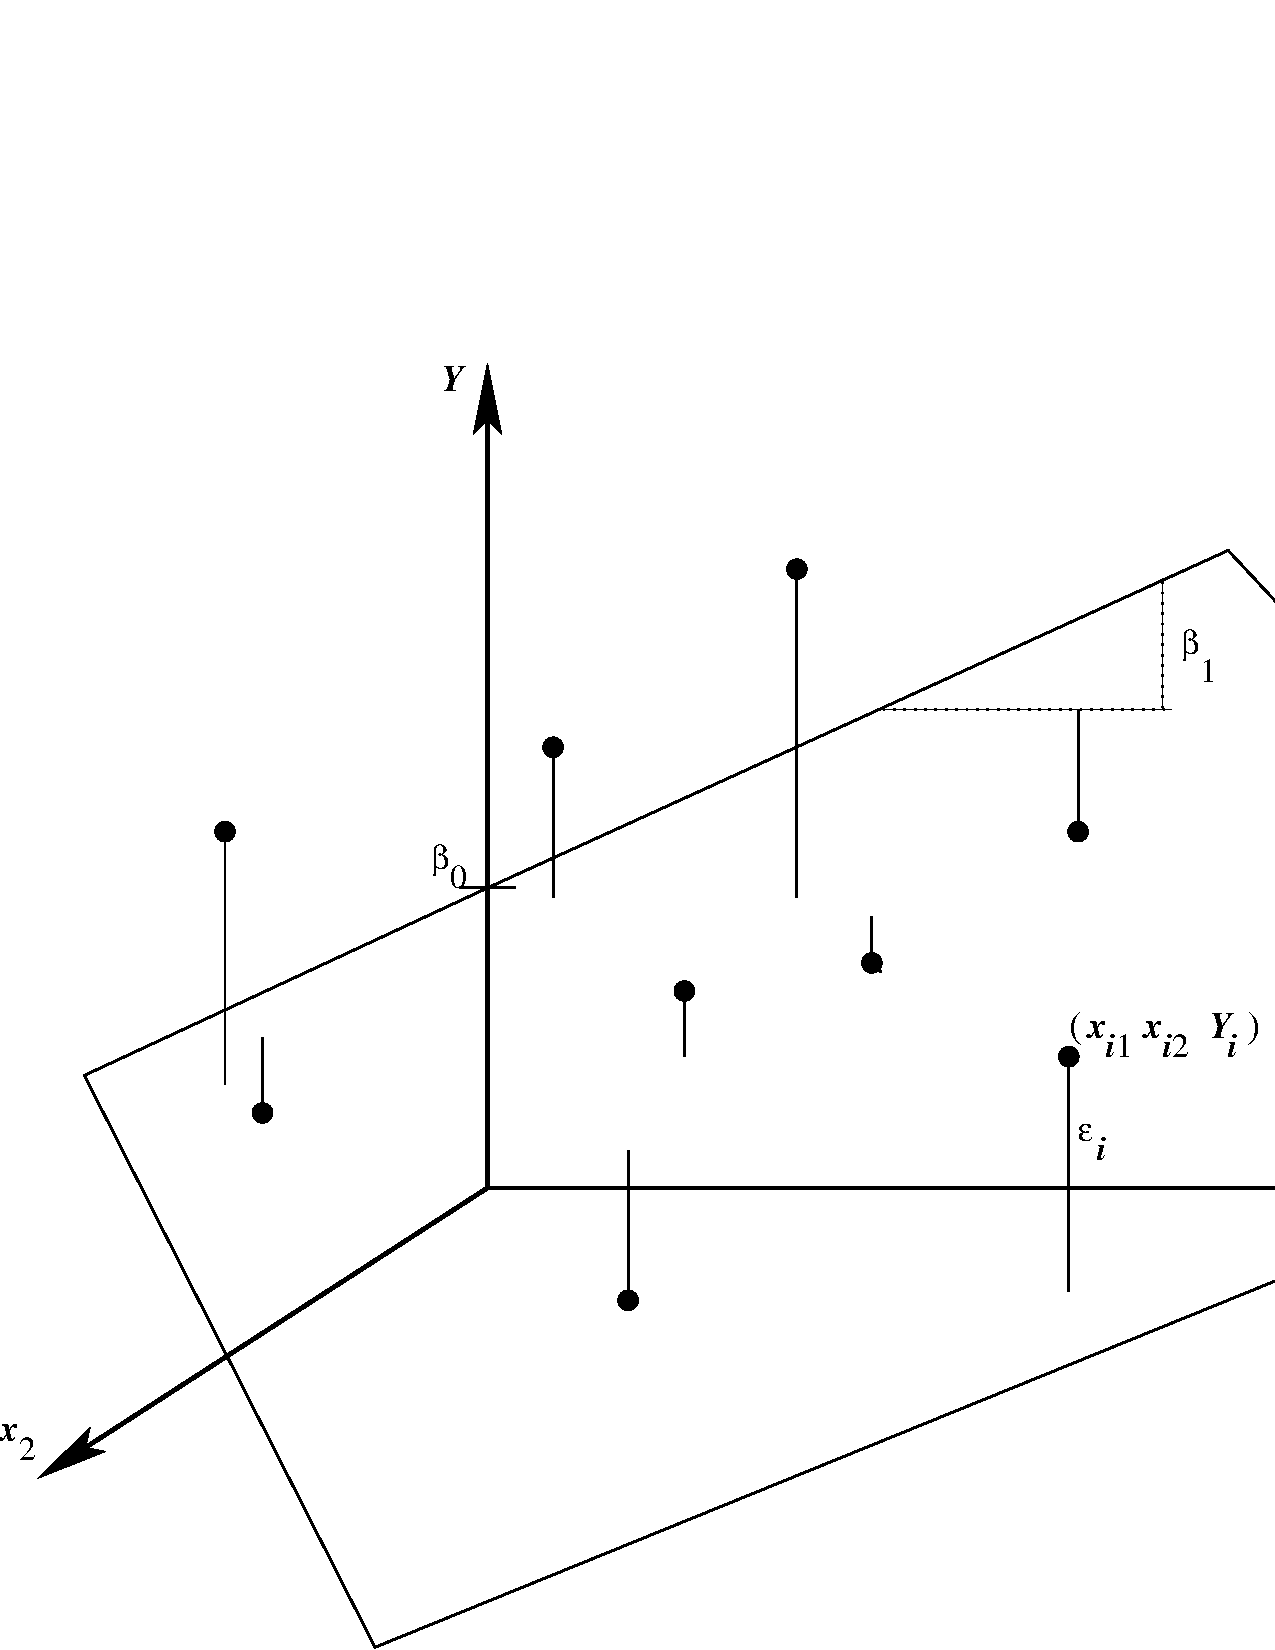
\includegraphics[scale=0.35, trim={0 0 0 5cm}]
{Chap5-AjusterRLM/Figures/reg_mult.pdf}}
\caption{Représentation géométrique du modèle de régression linéaire multiple.}\label{fig:rlm}
\end{figure}



\section{Estimation des coefficients}
\label{sec:EstimationParamètres}

%On présente ici de nouveau façons d'obtenir les estimateurs. Commenter sur la méthode du maximum de vraisemblance dans ce cas-ci; ça nous confirmerait qu'on a les meilleurs estimateurs possible. Noter également qu'on ne considère ici que les coefficients; on reviendra à l'estimation de la variance plus tard. }

\subsection{Méthode des moindres carrés}
\label{sec:EstimationRLMMoindresCarrés}


Comme dans le cas de la régression linéaire simple, on adopte à nouveau le principe des moindres carrés de Legendre. On cherche par conséquent le vecteur $\bobeta$ qui minimise la somme des carrés des résidus ($\sum_{i=1} ^n{\hat{\varepsilon}_i^2}$). Puisque le vecteur des résidus s'exprime
	\[ \hboeps= (\hat{\varepsilon}_1 , \hat{\varepsilon}_2, ... , \hat{\varepsilon}_n)' = \boY - \boX \hbobeta, \]
on a que
	\[\sum_{i=1}^n \hat{\varepsilon}_i^2= \hboeps' \hboeps= (\boY - \boX \hbobeta)' (\boY - \boX \bobeta)= f(\hbobeta)\]

En utilisant les propriétés des matrices (voir \ref{sec:prop_calc_mat}), $f(\hbobeta)$ s'écrit comme
\begin{eqnarray*}
	f(\hbobeta)&=&(\boY' - (\boX \hbobeta)')(\boY - \boX \hbobeta) \\
	&=& \boY' \boY - \boY' \boX \hbobeta - (\boX\hbobeta)' \boY + (\boX\hbobeta)' (\boX\hbobeta) \\
	&=& \boY' \boY - 2\hbobeta'\boX'\boY  + \hbobeta'\boX'  \boX\hbobeta
\end{eqnarray*}
Dans la dernière égalité on a utilisé le fait que $\boY'\boX\hbobeta=(\boX\hbobeta)'\boY=\hbobeta'\boX'\boY$, ce qu'on peut facilement démontrer puisque ces quantités sont des scalaires.

On obtient alors une fonction quadratique de $\hbobeta$. Pour minimiser $\sum_{i=1} ^n{\hat{\varepsilon}_i^2}$, on dérive $f(\hbobeta)$ par rapport à $\hbobeta$ et on pose $f'(\hbobeta)=0$ de la manière suivante :
\[
\begin{MAT}(r)[2pt,0pt,3cm]{c}
\frac{\partial f(\hbobeta)}{ \partial \hbobeta} \\
\end{MAT}
 = \left[
\begin{MAT}(r)[2pt,0pt,5.5cm]{c}
\frac{\partial f(\hbobeta)}{ \partial \hat{\beta}_0} \\
\frac{\partial f(\hbobeta)}{ \partial \hat{\beta}_1} \\
\vdots\\
\frac{\partial f(\hbobeta)}{ \partial \hat{\beta}_p} \\
\end{MAT}
\right] = \left[
\begin{MAT}(r)[2pt,0pt,5.5cm]{c}
0\\
0 \\
\vdots\\
0\\
\end{MAT}
\right]
\]
On obtient un système de $p+1$ équations à $p+1$ inconnues qu'il est possible d'exprimer sous format matriciel comme
	\[\frac{\partial f(\hbobeta)}{ \partial \hbobeta} = -2\boX' \boY + 2\boX' \boX \hbobeta =0\]

On veut donc résoudre $\boX' \boX \hbobeta = \boX' \boY$. Dans le cas où la matrice $\boX' \boX$ est inversible (de plein rang) on obtient que,
\begin{eqnarray}
	\underbrace{\hbobeta}_{(p+1)\times 1}=\underbrace{(\boX' \boX)^{-1}}_{(p+1)\times(p+1)} \underbrace{\boX'}_{(p+1)\times n} \underbrace{\boY}_{n\times 1}.
\label{eq:est_beta}
\end{eqnarray}

\begin{remarque}
La matrice $\boX' \boX$ n'est pas  inversible si le nombre d'observations $n$ est inférieur au nombre de paramètres à estimer $p'$, ou si une ligne de cette matrice est une combinaison linéaire des autres. Dans le premier cas, on pourra utiliser une méthode plus complexe, décrite à la section \ref{sub:lasso}. Dans le second cas, il faudra retirer cette variable du modèle. Voir aussi à cet effet le chapitre \ref{sec:Multicolinéarité} sur la multicolinéarité.
\end{remarque}


\subsubsection{Application au cas $p=1$}

Puisque le modèle de RLS est un cas particulier du modèle de RLM, il sera rassurant de vérifier que l'équation \ref{eq:est_beta} mène aux mêmes estimateurs que ceux de la section \ref{sec:AjusterRLS}.

Pour la RLS, la matrice d'incidence $\boX$ et sa transposée s'expriment comme :
\[
\begin{MAT}(r){c}
\boX\\
\end{MAT}
= \left[
\begin{MAT}(r){cc}
1 &  x_1\\
1 & x_2 \\
\vdots & \vdots  \\
1 & x_n \\
\end{MAT}
 \right]
\begin{MAT}(r){c}
\boX' \\
\end{MAT}
= \left[
\begin{MAT}(r){ccc}
1 & \ldots & 1\\
x_1 & \cdots & x_n \\
\end{MAT}
\right]
\]

On commence par calculer $\boX' \boX$.
\[
\begin{MAT}(e){c}
\boX' \boX\\
\end{MAT}
 = \left[
\begin{MAT}(e)[2pt,0pt,3cm]{cc}
n &  \sum_{i=1}^n x_i  \\
\sum_{i=1}^n x_i & \sum_{i=1}^n x_i^2 \\
\end{MAT}
\right] = \left[
\begin{MAT}(e)[2pt,0pt,3cm]{cc}
n & n\overline{x}\\
n\overline{x} & \sum_{i=1}^n x_i^2 \\
\end{MAT}
\right]
\]

Puis on trouve son inverse en se basant sur la formule d'inversion d'une matrice de dimension $2\times 2$. La première étape consiste à calculer le déterminant
$$	\mbox{det}(\boX'\boX) = n \sum_{i=1}^n x_i^2 - n^2\overline{x}^2
	= n \left(\sum_{i=1}^n x_i^2 - \sum_{i=1}^n \overline{x}^2\right)
	= n \sum_{i=1}^n  (x_i^2 - \overline{x}^2)
	= n \sum_{i=1}^n  (x_i - \overline{x})^2
	= n S_{xx}
$$

On a donc
\[
\begin{MAT}{c}
(\boX' \boX) ^{-1}\\
\end{MAT}
 =
\begin{MAT}{c}
\frac{1}{nS_{xx}}\\
\end{MAT}
\left[
\begin{MAT}(e){cc}
\sum_{i=1}^n x_i^2 & -n\overline{x}\\
-n\overline{x} & n \\
\end{MAT}
\right]
\]

On peut ensuite calculer $\hbobeta= (\boX' \boX)^{-1} \boX' \boY$.
\begin{align*}
\begin{MAT}{c}
\hbobeta \\
\end{MAT}
&= \frac{1}{nS_{xx}} \left[
\begin{MAT}{cc}
\sum_{i=1}^n x_i^2 & -n\overline{x}\\
-n\overline{x} & n \\
\end{MAT}
\right] \left( \left[
\begin{MAT}{cccc}
1 & 1 & \ldots &1 \\
x_1 & x_2 & \cdots & x_n\\
\end{MAT}
\right] \left[
\begin{MAT}{c}
Y_1 \\
Y_2 \\
\vdots \\
Y_n \\
\end{MAT}
\right] \right) \\
%
&
= \frac{1}{nS_{xx}} \left[
\begin{MAT}{cc}
\sum_{i=1}^n x_i^2 & -n\overline{x}\\
-n\overline{x} & n \\
\end{MAT}
\right] \left[
\begin{MAT}{c}
\sum_{i=1}^n Y_i \\
\sum_{i=1}^n x_i Y_i \\
\end{MAT}
\right]\\
%
& = \frac{1}{nS_{xx}} \left[
\begin{MAT}{c}
\sum_{i=1}^n x_i^2 n\overline{Y} - \sum_{i=1}^n x_i Y_i n\overline{x} \\
-\sum_{i=1}^n Y_i n\overline{x} + n \sum_{i=1}^n x_i Y_i\\
\end{MAT}
\right]
\end{align*}

On obtient donc
\begin{eqnarray*}
	\hat{\beta}_1 &=& \frac{n \sum_{i=1}^n x_i Y_i - n^2\overline{x} \overline{Y}}{n S_{xx}}= \frac{S_{xy}}{S_{xx}}.
\end{eqnarray*}

Pour l'ordonnée à l'origine, on a
\begin{eqnarray*}
	\hat{\beta}_0 &=& \frac{n \overline{Y} \sum_{i=1}^n x_i^2 - n\overline{x} \sum_{i=1}^n x_i Y_i}{nS_{xx}}
\end{eqnarray*}
En ajoutant $n\overline{x}^2\overline{Y} -n\overline{x}^2\overline{Y}$ au numérateur, on obtient que
\begin{eqnarray*}
		\hat{\beta}_0 & = & \frac{\overline Y(\sum x_i^2-n\overline x^2)-\overline x(\sum x_i Y_i-n\overline x\overline Y)}{S_{xx}} \\
       &=& \frac{\overline{Y}S_{xx} - \overline{x}S_{xy}}{S_{xx}} \\
	&=& \overline{Y} - \overline{x} \hat{\beta}_1 .
\end{eqnarray*}
On obtient donc exactement les mêmes résultats qu'en \eqref{eq:dbeta0egal0}.  et \eqref{eq:beta1}.

\begin{remarque}
De façon plus générale, en RLM,
\begin{eqnarray*}
	\hat{\beta}_0 &=& \overline{Y} - \overline{x}'_* \hat{\beta}_*\\
	&=& \overline{Y} - \sum_{i=1}^p \hat{\beta}_i \overline{x}^*_i
\end{eqnarray*}
où $\hat{\beta}_*$ est le vecteur des coefficients amputé de $\hat{\beta}_0$ et $\overline{X}_*$ est le vecteur contenant la moyenne de chaque variable (sans la colonne de 1).
\end{remarque}


\subsection{Argument géométrique}
\label{sec:ArgumentGéométrique}

Voyons maintenant comment arriver à \ref{eq:est_beta} à l'aide d'un argument géométrique.

Dans le modèle de régression linéaire multiple, on cherche à écrire $\boY$ comme une combinaison linéaire des colonnes de $\boX$, plus une erreur $\boeps$. Autrement dit, on veut projeter $\boY$ dans le sous-espace vectoriel engendré par $\boX$. Si $\boX$ est de plein rang (inversible), cet espace aura $p'=p+1$ dimensions.

On appelle matrice chapeau la matrice de projection de $\boY$ dans l'espace de $\boX$, et on la dénote $\boH$ (voir la section \ref{sec:MatriceChapeau} pour plus de détails sur cette matrice). Le vecteur résiduel défini par $\hboeps = \boY-\hY = (\boI_n-\boH)\boY$ est alors perpendiculaire à l'espace engendré par $\boX$. La figure \ref{fig:geometrie} représente géométriquement le cas à 3 observations $\boY=(Y_1,Y_2,Y_3)$ où l'on a deux paramètres à estimer ($p'=2$).

\begin{figure}[htb!]
	\centering
		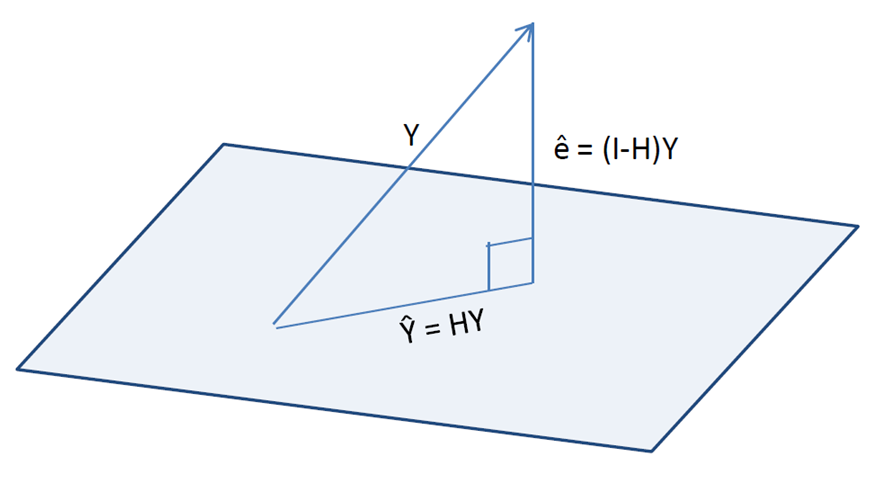
\includegraphics[scale = 0.9]{Chap5-AjusterRLM/Figures/geometrie}
	\caption{Représentation géométrique de la régression dans le cas où il y a deux paramètres à estimer.}
	\label{fig:geometrie}
\end{figure}

%Si $\boX$ n'est pas de plein rang, certaines colonnes de $\boX$ (certaines variables) sont linéairement dépendantes. Dans ce cas, il suffit de retirer une ou plusieurs variables.

Le vecteur des résidus est la projection de $\boY$ dans l'espace perpendiculaire à $\boX$. Toujours en considérant $\boX$ de plein rang, cet espace est de dimension $(n-p')$.

L'angle droit entre le vecteur des valeurs prédites ($\hY$) et le vecteur des résidus $\hboeps$ découle du fait que l'on ait choisi $\hbobeta$ de façon à minimiser la somme des résidus au carré, c'est-à-dire $\hboeps'\hboeps$. L'orthogonalité de $\hY$ et $\hboeps$ revient à dire que $\cov[\hboeps, \hY] = 0$. En effet, des vecteurs orthogonaux sont des vecteurs non corrélés. Dans le cas gaussien, ceci implique de plus que ces vecteurs sont indépendants.


Cette approche permet de refaire le calcul nous ayant mené \`a la formule pour $\hbobeta$. En effet, les résidus sont perpendiculaires au plan, car on souhaite faire une projection orthogonale. On peut donc dire qu'ils sont orthogonaux aux combinaisons linéaires des colonnes de $\boX$, en particulier à $\boX$ lui-même. Pour trouver la valeur de $\hbobeta$ telle
que $\boX$ est orthogonal \`a $\hboeps$, on doit résoudre
\begin{equation}\label{eqnorm:geo}
\boX'\hboeps=\boX'(\boY-\boX\hbobeta)=\bo{0}.
\end{equation}


On arrive donc tel que prévu à
$$\hbobeta=(\boX'\boX)^{-1}\boX'\boY.$$

\subsection{Méthode du maximum de vraisemblance}
\label{sec:RLM-MLE}

Comme pour la RLS, l'estimateur en \ref{eq:est_beta} peut être obtenu à l'aide de la méthode du maximum de vraisemblance. Nous omettons les détails ici.

La méthode du maximum de vraisemblance permet également d'estimer $\sigma^2$. Comme pour la RLS, l'estimateur du maximum de vraisemblance pour la variance des erreurs est toutefois biaisé. Nous utiliserons plutôt un estimateur non-biaisé de cette variance, lequel est dérivé à la section
\ref{sec:RLM-sigma}.

\newpage

\section{Exemple}

Cet exemple est tiré de \citet[][Exemple 14.1]{Hin_Mon_Gol_Bor:12}.
%\citet{Rag_Ber:01} exposent une analyse consistant à trouver un modèle de prévision des meurtrissures des pommes durant le tri et l'emballage.
Des expériences en laboratoire ont montré que le diamètre des meurtrissures (en mm) peut être expliqué en fonction de la hauteur de chute (en mm) et de la masse volumique des fruits (en g/cm$^3$). Le Tableau \ref{exp_data} présente des données typiques de ce type d'expérience.


\begin{table}[htb!]
\caption{Données pour l'exemple des meurtrissures de pêches}
\label{exp_data}
\begin{tabular}{|c|c|c|c|} \hline
numéro &  diamètre des meurtrissures  & hauteur de chute  & masse volumique  \\
 & [mm] & [mm] & [g/cm$^3$] \\
        & $Y_i$        & $x_{i1}$      &  $x_{i2}$ \\ \hline
 1   &   3,62  &   303,7  & 0,90      \\
 2   &   7,27  &   366,7  & 1,04     \\
 3   &   2,66  &  336,8   & 1,01     \\
 4   &   1,53  &  304,5   & 0,95      \\
 5   &   4,91  &  346,8   & 0,98      \\
 6   &   10,36 &   600,0    & 1,04       \\
 7   &   5,26  &   369,0    & 0,96       \\
 8   &   6,09  &   418,0    & 1,00           \\
 9   &   6,57  &   269,0    & 1,01        \\
 10  &   4,24  &   323,0    & 0,94         \\
 11  &   8,04  &   562,2  & 1,01          \\
 12  &   3,46  &   284,2  & 0,97           \\
 13  &   8,50   &   558,6  & 1,03           \\
 14  &   9,34  &   415,0    & 1,01            \\
 15  &   5,55  &   349,5  & 1,04            \\
 16  &   8,11  &   462,8  & 1,02            \\
 17  &   7,32  &   333,1  & 1,05            \\
 18  &   12,58 &   502,1  & 1,10            \\
 19  &   0,15  &   311,4  & 0,91            \\
 20  &   5,23  &   351,4  & 0,96            \\   \hline
\end{tabular}

\end{table}


Le modèle de régression linéaire multiple s'exprime sous forme matricielle comme


$$
\underbrace{\left(
\begin{array}{c}
3,62  \\
7,27  \\
2,66 \\
1,53 \\
\vdots \\
5,23  \\
\end{array} \right)}_{20\times 1}
 =  \underbrace{\left(\begin{array}{ccc}
            1	&      303,7  & 0,9     \\
            1	&      366,7  & 1,04    \\
            1 &         336,8 & 1,01 \\
            1 &           304,5 & 0,95 \\
            \vdots & \vdots & \vdots   \\
            1	&      351,4  & 0,96
\end{array}\right)}_{20\times 3}
\underbrace{\left(\begin{array}{c}
\beta_0 \\
\beta_1 \\
\beta_2
\end{array} \right)}_{3\times 1}+
\underbrace{\left(\begin{array}{c}
\varepsilon_1 \\
\varepsilon_2 \\
\varepsilon_3 \\
\varepsilon_4 \\
\vdots \\
\varepsilon_{20}
 \end{array}
 \right)}_{20\times 1}
 $$


Selon l'équation \ref{eq:est_beta}, on sait que $\hbobeta=(\boX'\boX)^{-1}\boX' \boY$.

La matrice $\boX'\boX$ est
\begin{eqnarray*}
\boX'\boX & = & \left(
\begin{array}{cccc}
1 & 1 & \cdots & 1 \\
303,7 & 366,7 & \cdots & 351,4 \\
0,90 & 1,04 & \cdots & 0,96
\end{array}
\right)
\left(
\begin{array}{ccc}
1 & 303,7 & 0,90 \\
1 & 366,7 & 1,04 \\
\vdots & \vdots & \vdots \\
1 & 351,4 & 0,96
\end{array}
\right) \\
& = & \left(
\begin{array}{ccc}
20 & 7767,8 & 19,33 \\
7767,8 & 3201646 & 7791,878 \\
19,93 & 7791,878 & 19,9077
\end{array}
\right).
\end{eqnarray*}
Le vecteur $\boX'\boY$ s'exprime comme
\begin{eqnarray*}
\left(
\begin{array}{cccc}
1 & 1 & \cdots & 1 \\
303,7 & 366,7 & \cdots & 351,4 \\
0,90 & 1,04 & \cdots & 0,96
\end{array}
\right)
\left(
\begin{array}{c}
3,62 \\
7,27 \\
\vdots \\
5,23
\end{array}
\right)
=
\left(
\begin{array}{r}
120,79 \\
51129,17 \\
122,70
\end{array}
\right).
\end{eqnarray*}
On en déduit donc que
\begin{eqnarray*}
\left(
\begin{array}{c}
\hat\beta_0 \\
\hat\beta_1 \\
\hat\beta_2
\end{array}
\right)
& = &
\left(
\begin{array}{ccc}
20 & 7767,8 & 19,33 \\
7767,8 & 3201646 & 7791,878 \\
19,93 & 7791,878 & 19,9077
\end{array}
\right)^{-1}
\left(
\begin{array}{r}
120,79 \\
51129,17 \\
122,70
\end{array}
\right) \\
& = &
\left(
\begin{array}{rrr}
24,63666 & 0,005321 & -26,74679 \\
0,005321 & 0,0000077 & -0,008353 \\
-26,74679 & -0,008353 & 30,096389
\end{array}
\right)
\left(
\begin{array}{r}
120,79 \\
51129,17 \\
122,70
\end{array}
\right) \\
& = &
\left(
\begin{array}{r}
-33,8310 \\
0,0134 \\
34,8900
\end{array}
\right)
\end{eqnarray*}
Par conséquent, le modèle de régression ajusté s'écrit comme
$$\hat Y=-33,831+0,0134x_1+34,890x_2.$$
L'espérance du diamètre moyen des meurtrissures d'une pêche de masse volumique nulle lancée d'une hauteur nulle (très hypothétique comme valeur!) est de $-33,831$ mm. L'augmentation d'un mm de la hauteur de la chute est associée à une augmentation attendue de 0,0134 mm du diamètre moyen des meurtrissures, pour une masse volumique constante. De même, l'augmentation d'un $g/cm^3$ de la masse volumique d'une pêche est associée à une augmentation attendue de $34,890$ mm du diamètre moyen des meurtrissures, pour une hauteur de chute constante.



\chapter{Inférence pour la RLM}
\label{sec:InferenceRLM}


\section{Distribution de l'estimateur}

Comme dans le cas de la RLS, on utilisera la distribution des estimateurs pour dériver les méthodes d'inférence.  Pour trouver la loi des estimateurs, on doit faire l'hypothèse que la matrice des termes d'erreurs $\boeps$ est distribuée selon une loi normale multivariée de dimension égale au nombre d'observations $n$. Une brève introduction à cette distribution multivariée est présentée à l'annexe \ref{LaLoiNormaleMultivariée}.

On peut écrire cette hypothèse sous la forme
$$\boeps=[\varepsilon_1,\varepsilon_2,...,\varepsilon_n]' \sim \N_n(\textbf{0}, \sigma^2\boI_n)$$
où  $\boI_n$ dénote la matrice identité de dimension $n\times n$.

On a donc que
\begin{eqnarray*}
	\boY \sim \N_n (\boX\bobeta, \sigma^2 \boI_n).
\end{eqnarray*}

Afin de déterminer l'espérance et la variance de $\hbobeta$ on suit la même approche que pour la régression linéaire simple et on exprime $\hbobeta$ comme une combinaison linéaire des $Y_i$.


On a vu que
\begin{eqnarray*}
	\hbobeta=(\boX'\boX)^{-1}\boX'\boY
\end{eqnarray*}
On a donc que $\hbobeta \sim \N_p(\esp[\hbobeta],\var[\hbobeta])$ car une combinaison linéaire de variables aléatoires normales est également normalement distribuée. Il suffit donc de calculer $\esp[\hbobeta]$ et $\var[\hbobeta]$ afin que la distribution soit entièrement déterminée.

On peut d'abord montrer que l'estimateur est non biaisé:
\begin{eqnarray*}
	\esp[\hbobeta]&=&\esp[(\boX'\boX)^{-1}\boX'\boY] \\
	&=& (\boX'\boX)^{-1}\boX' \esp[\boY]\\
	&=& (\boX'\boX)^{-1}\boX' \boX\bobeta\\
	&=& \bobeta
\end{eqnarray*}
On calcule ensuite la variance:
\begin{eqnarray*}
	\var[\hbobeta]&=& \var[(\boX'\boX)^{-1}\boX'\boY]\\
	&=& (\boX'\boX)^{-1}\boX' \var[\boY] \left\{(\boX'\boX)^{-1}\boX'\right\}'\\
	&=& (\boX'\boX)^{-1}\boX' \sigma^2\boI_n \left\{(\boX'\boX)^{-1}\boX'\right\}'\\
	&=& \sigma^2 (\boX'\boX)^{-1} \boX' \boX(\boX'\boX)^{-1}\\
	&=& \sigma^2 (\boX'\boX)^{-1}
\end{eqnarray*}
Donc,
\begin{eqnarray}
	\hbobeta \sim \N_p\{\bobeta,\sigma^2 (\boX'\boX)^{-1}\}
	\label{loibeta}
\end{eqnarray}


\subsubsection{Application au cas $p=1$}
\label{sec:VarCovDesEstimateur}

On a déjà vu que dans le cas où $p=1$,

\begin{equation}
\label{invxtx}
\begin{MAT}{c}
(\boX' \boX) ^{-1}\\
\end{MAT}
 =
\begin{MAT}{c}
\frac{1}{nS_{xx}}\\
\end{MAT}
\left[
\begin{MAT}(e){cc}
\sum_{i=1}^n x_i^2 & -n\bar{x}\\
-n\bar{x} & n \\
\end{MAT}
\right].
\end{equation}

À partir de \eqref{loibeta} et \eqref{invxtx}, on peut calculer les variances et la covariance de $\hat{\beta}_0$ et de $\hat{\beta}_1$.

\begin{eqnarray*}
	\var[\hat{\beta}_1]&=&\frac{\sigma^2 n}{n S_{xx}} = \frac{\sigma^2}{S_{xx}}\\
	\var[\hat{\beta}_0]&=&\frac{\sigma^2 \sum_{i=1}^n x_i^2}{n S_{xx}}\\
	\cov[\hat{\beta}_1,\hat{\beta}_0]&=& \frac{-n\bar{x} \sigma^2}{n S_{xx}}= \frac{-\bar{x} \sigma^2}{S_{xx}}
\end{eqnarray*}

On obtient les variances déjà connues. Remarquez que la covariance entre $\hat{\beta}_0$ et $\hat{\beta}_1$ est de signe contraire de $\bar{x}$ et que cette covariance est nulle si $\bar{x}=0$. %Dans le cas où $p=2$, on trouve
%%
%
%\begin{eqnarray*}
%		f(X_1,X_2)= \left(\frac{1}{\sqrt{2\pi}}\right)^2 \frac{1}{\left|\Sigma\right|^{1/2}} \exp\left(-\frac{1}{2} (X- \mu)^T \Sigma^{-1} (X- \mu)\right)\\
%		= \left(\frac{1}{\sqrt{2\pi}}\right)^2 \frac{1}{\sigma_1\sigma_2\sqrt{1-r^2}} e^{ -\frac{1}{2 (1-r^2)} \left(\frac{x_1- \mu_1}{\sigma_1}\right)^2 +\left(\frac{x_2- \mu_2}{\sigma_2}\right)^2 - 2r\left(\frac{x_1- \mu_1}{\sigma_1}\right)\left(\frac{x_2- \mu_2}{\sigma_2}\right)}
%\end{eqnarray*}
%
%Le dernier terme de l'exponentielle est un terme croisé qui induit la corrélation; il est nul lorsque $r$, la corrélation entre $X_1$ et $X_2$ est égale à zéro.



\section{Matrice chapeau et implications}
\label{sec:MatriceChapeau}

On a introduit la matrice chapeau à la section \ref{sec:ArgumentGéométrique}. Cette matrice est très importante dans la RLM. Dans cette section, on explore plus en détails la matrice chapeau, et on obtient quelques résultats utiles pour l'inférence à partir de ses propriétés.

\subsection{La matrice chapeau}
\label{sec:LaMatriceChapeau}

La matrice chapeau $\boH$ («hat matrix») tire son nom du fait qu'elle permet de transformer $\boY$ en $\hY$ ("Y chapeau"). On va déterminer cette matrice. Selon l'équation \eqref{eq:reg_lin_mult_mat}, la régression linéaire multiple s'exprime sous format matriciel comme $\boY = \boX\bobeta + \boeps$.
L'estimateur de $\bobeta$ peut s'écrire selon l'équation \eqref{eq:est_beta} comme $\hbobeta = (\boX'\boX)^{-1}\boX'\boY$. On obtient donc que
\begin{eqnarray*}
	\hY& =& \boX\hbobeta \\
    &= & \boX(\boX'\boX)^{-1}\boX'\boY=\boH\boY
\end{eqnarray*}
La matrice chapeau correspond donc à la matrice $\boH=\boX(\boX'\boX)^{-1}\boX'$.


Il est également possible d'exprimer les résidus en fonction de la matrice chapeau de la manière suivante :
	\[\hboeps=\boY-\hY = (\boI_n- \boX(\boX'\boX)^{-1}\boX')\boY = (\boI_n-\boH)\boY
\]

% a continuer ici
La matrice chapeau peut être vue comme une matrice de transformation. Il s'agit d'un opérateur linéaire, de même que ($\boI_n-\boH$). Ces deux opérateurs possèdent plusieurs propriétés intéressantes, à savoir :

\begin{enumerate}
   \item $\boH'=\boH$ (symétrie)
	\item $\boH\boH=\boH$ (idempotence)
	\item $\boH\boX=\boX$
     \item $(\boI_n-\boH)'=(\boI_n-\boH)$ (symétrie)
	\item $(\boI_n-\boH)(\boI_n-\boH)=(\boI_n-\boH)$ (idempotence)
	\item $(\boI_n-\boH)\boX=0$
\end{enumerate}

De plus, tous les éléments de la matrice ont une interprétation précise et utile pour étudier la robustesse d'un modèle de RLM. Nous y reviendrons à la section \ref{sec:DonneesInfluentes}.


\subsection{Distribution de $\hat{Y}$ et $\hat{\varepsilon}$}
\label{sec:distYhatEps}

Les propriétés de la matrice chapeau permettent de calculer la variance de $\hY$ et $\hboeps$.
En effet,
\begin{eqnarray*}
	\var[\hY] = \var[\boH\boY]=\boH'\var[\boY]\boH= \boH\boH \sigma^2 = \boH \sigma^2
\end{eqnarray*}
et
\begin{eqnarray*}
	\var[\hboeps]=\var[(\boI_n-\boH)\boY]= (\boI_n-\boH)\sigma^2
\end{eqnarray*}

On a donc que les lois de $\hY$ et $\hboeps$ sont respectivement
\begin{eqnarray*}
	\hY \sim \N_n(\boX\bobeta, \sigma^2\boH)
\end{eqnarray*}
\begin{eqnarray}
	\hboeps \sim \N_n(0, \sigma^2(\boI_n-\boH)).
	\label{distepsilon}
\end{eqnarray}


\subsection{Estimation de $\sigma^2$}
\label{sec:RLM-sigma}

Comme on a indiqué à la section \ref{sec:RLM-MLE}, la méthode du maximum de vraisemblance permet de trouver un estimateur pour $\sigma^2$, mais celui-ci est biaisé. On utilisera plutôt l'estimateur suivant:
\begin{eqnarray}
	\hat{\sigma^2}=\frac{\hboeps'\hboeps}{n-p'}
	\label{estimationSigma}
\end{eqnarray}

où $p'=p+1$.

On utilisera ici le résultat \ref{distepsilon} pour prouver que \ref{estimationSigma} est non biaisé pour $\sigma^2$.


On veut donc prouver que
$$ E \left( \frac{\hboeps'\hboeps}{n-p'} \right) = \sigma^2. $$

Puisque $\hboeps \sim \N_n(0, \sigma^2(\boI_n-\boH))$, on peut écrire
$$ \frac{\hboeps}{\sigma} \sim \N_n(0, (\boI_n-\boH)).$$

On peut également écrire
$$ \frac{\hboeps}{\sigma} = (\boI_n - \boH)\bo Z \mbox{    o\`u  } \bo Z \sim \N_n(\bo 0, \boI_n).$$

\newpage
Cette forme nous permet d'utiliser le théorème suivant:

\textcolor{red}{ XXXX \\ A changer, le thm est dans le chapitre 4  maintenant. \\ XXXX}

\begin{theorem}
Si $\boY \sim \N_n(\bo 0,\boI_n)$ et $\bo A$ est une matrice symétrique, alors $\boY'\bo A\boY \sim \chi^2_r$ si et seulement si $\bo A$ est idempotente de rang r.
\end{theorem}

En effet, puisque
\begin{itemize}
\item[$\bullet$] $\bo Z \sim \N_n(\bo 0,\boI_n)$
\item[$\bullet$] $(\boI_n-\boH)$ est symétrique
\item[$\bullet$] $(\boI_n-\boH)$ est idempotente
\end{itemize}
alors, on a que
$$ \bo Z'(\boI_n-\boH) \bo Z \sim \chi^2_r$$
avec $r$ = rang$(\boI_n-\boH) = n-p'$. \\

%Si on connaît $\sigma$, il est alors possible d'utiliser ce résultat pour construire un intervalle de confiance sur $\beta_i$ ou pour faire des test d'hypothèses. Or en pratique, $\sigma$ est généralement inconnu. On l'estimera alors par

Or,
\begin{align*}
\bo Z'(\boI_n-\boH) \bo Z &= \bo Z'(\boI_n-\boH)'(\boI_n-\boH) \bo Z \\
&= ((\boI_n-\boH)\bo Z)' (\boI_n-\boH) \bo Z \\
&= \frac{\hboeps'}{\sigma} \frac{\hboeps}{\sigma} \\
&= \frac{\hboeps'\hboeps}{\sigma^2}
\end{align*}


Ainsi,
$$ \frac{\hboeps'\hboeps}{\sigma^2} \sim \chi^2_r$$
avec $r$ = rang$(\boI_n-\boH) = n-p'$. \\

On peut donc facilement prouver le résultat voulu:

\begin{align*}
E \left( \frac{\hboeps'\hboeps}{\sigma^2} \right) &= n-p' \\
E \left( \hboeps'\hboeps \right) &= \sigma^2 (n-p') \\
E \left( \frac{\hboeps'\hboeps}{n-p'} \right) &= \sigma^2
\end{align*}


\section{Intervalle de confiance et test d'hypothèse pour un coefficient}
\label{sec:infbetaRLM}

On a vu que du postulat de normalité $\boeps \sim \N_n(0,\sigma^2\boI_n)$, découle que $\hbobeta \sim \N_p(\bobeta,\sigma^2 (\boX'\boX)^{-1})$ (équation \ref{loibeta}). Si on s'intéresse à un $\beta_i$ en particulier, on a alors que
\begin{eqnarray*}
	\frac{\hat{\beta}_i-\beta_i}{\sigma \sqrt{v_{ii}}} \sim \N(0,1)
\end{eqnarray*}

où $v_{ii}$ est l'élément $(i,i)$ de la matrice $(\boX'\boX)^{-1}$.



On vient de montrer que $\frac{\hboeps'\hboeps}{n-p'}$ est un estimateur sans biais de $\sigma^2$. De plus, cet estimateur est indépendant de $\hbobeta$. Par conséquent,
\begin{eqnarray}
	\frac{\frac{\hat{\beta}_i-\beta_i}{\sigma \sqrt{v_{ii}}}}{\sqrt{\frac{\hboeps'\hboeps}{\sigma^2(n-p')}}} \sim \frac{\N(0,1)}{\sqrt{\chi^2_{n-p'}/(n-p')}} \sim \mathcal{T}_{n-p'}
	\label{loistudentbeta}
\end{eqnarray}

où $\mathcal{T}_{n-p'}$ note la loi de Student à $n-p'$ degrés de liberté. On peut alors utiliser \eqref{loistudentbeta} pour construire un intervalle de confiance pour $\bobeta$ ou pour effectuer des tests d'hypothèses.

Ainsi, l'intervalle de confiance de niveau $(1-\alpha)$ pour $\beta_i$ s'exprime comme
\begin{eqnarray}
\left[ \hat\beta_i\pm t_{n-p';1-\alpha/2}\sqrt{\hat\sigma^2 v_{ii}} \right]
\label{intconf_beta}
\end{eqnarray}

\begin{exemple}
Construisons un intervalle de confiance à 95 $\%$ pour le paramètre $\beta_1$ de l'exemple de la section \ref{exp_data}. Nous avons déjà calculé que $\hat\beta_1=0,01314$. L'élément diagonal de la matrice $\boX'\boX$ correspondant à $\beta_1$ est $v_{22}=0,0000077$. L'estimation non biaisée de $\sigma^2$ est $\hat\sigma^2=2,247$. Le quantile à 97,5 $\%$ d'une loi $\mathcal{T}$ de Student à $n-p'=20-3=17$ degrés de liberté est égal à 2,110.  On obtient donc selon \eqref{intconf_beta} l'intervalle de confiance suivant :
\begin{align*}
\left[ \hat\beta_1\pm t_{n-p'; 1-\alpha/2}\sqrt{\hat\sigma^2 v_{22}} \right] &=\left[0,01314\pm2,110\sqrt{2,247\times 0,0000077}\right]\\
&=[0,00436;0,0219]
\end{align*}
On note que l'intervalle n'inclut pas la valeur 0. On peut donc rejeter l'hypothèse nulle $H_0: \beta_1=0$  et conclure que la hauteur de la chute est significativement associée au diamètre moyen des meurtrissures, en tenant compte de la présence des autres variables explicatives dans le modèle.
\end{exemple}


\section{Prévision}
\label{sec:PrévisionRLM}


Quand on veut faire une prévision, on s'intéresse à une combinaison linéaire des coefficients. Considérons donc le problème général d'estimer une combinaison linéaire de $\bobeta$:
\begin{equation}
\sum_{i=0}^p a_i \beta_i = \bo a'\bobeta
	\hspace{1cm} \mbox{o\`u} \hspace{1cm} \bo a'=[a_0\ a_1 \ ... \ a_p].
\label{eq:abeta}
\end{equation}
	
Intuitivement, on utiliserait $\bo a'\hbobeta$ comme estimateur. Et en effet, on sait que
\begin{equation}
\bo a'\hbobeta \sim \N(\bo a'\bobeta, \sigma^2\bo a'(\boX'\boX)^{-1}\bo a)
\label{eq:distabeta}
\end{equation}
On utilisera ce résultat pour la prévision.
% et donc cet estimateur est sans biais. On utilisera ce r
%La prévision s'obtient donc comme pour la RLS en remplaçant dans le modèle de régression chaque coefficient par son estimé.

% \textcolor{red}{Dois-je expliquer un peu plus pourquoi?} Cet estimateur n'est donc pas biaisé. Montrons d'abord qu'il est le meilleur estimateur non biaisé.

\subsection{Inférence sur  $\bo a'\bobeta$ }
\label{sec:TestsDHypothèsetheta}

%Notons que la forme de l'équation \ref{eq:beta} est très générale. Elle s'applique pour obtenir une prévision, mais également pour toute combinaison linéaire des coefficients.On peut donc utiliser le résultat \ref{eq:distabeta} pour obtenir un intervalle de confiance pour une combo linéaire des coeff

On peut utiliser (\ref{eq:distabeta}) pour faire de l'inférence sur une combinaison linéaire des coefficients.

Si on connaissait $\sigma^2$, on pourrait construire des intervalles de confiance et des tests d'hypothèses pour $\bo a'\bobeta$ à partir de
\begin{eqnarray}
	\frac{\bo a'\hbobeta-\bo a'\bobeta}{\sqrt{\sigma^2\bo a'(\boX'\boX)^{-1}\bo a}} \sim \N(0,1).
\end{eqnarray}

Toutefois, comme on ne connaît pas $\sigma^2$, on l'estimera par $\hat{\sigma^2}=\frac{\hboeps'\hboeps}{n-p'}$ (équation \ref{estimationSigma}) et on procèdera comme pour l'équation \ref{loistudentbeta} pour trouver que
\begin{eqnarray}
		\frac{\bo a'\hbobeta-\bo a'\bobeta}{\sqrt{\hat{\sigma}^2\bo a'(\boX'\boX)^{-1}\bo a}} \sim \mathcal{T}_{n-p'}.
		\label{distprevision}
\end{eqnarray}

On peut alors utiliser ce résultat pour construire un intervalle de confiance pour $\bo a'\bobeta$ ou pour tester $H_0: \bo a'\bobeta=c$.

\begin{remarque}
Il y a plusieurs circonstances dans lesquelles on voudrait faire de l'inférence sur une combinaison linéaire des coefficients. On pourrait se demander si une variable a un effet aussi grand qu'une autre (on s'intéresse alors à $\beta_i - \beta_j$), ou si une variable a un effet deux fois plus grand qu'une autre ($\beta_i - 2\beta_j$), par exemple. Le résultat \ref{distprevision} s'applique aussi dans le cas de la prévision pour de nouvelles observations, comme on verra plus bas.
\end{remarque}


\subsection{Inférence sur $\esp[Y|\bo{x}]$}
\label{sec:previsionRLM1}

On désire dans ce cas estimer la valeur moyenne de la
variable endog\`ene pour une combinaison de valeurs
$\bo{x^*}'=(x_1^*,\ldots,x_{p}^*)$ spécifiées des variables
exog\`enes. On veut donc estimer
$\esp[Y|\bo{x^*}]=\esp[\bo{x^*}'\bobeta+\varepsilon]=\bo{x^*}'\bobeta$.
Cela revient donc à estimer une combinaison linéaire de $\bobeta$ et il suffit de  remplacer $\bo{x^*}'$ par $\bo a'$ dans la section ci-dessus
afin d'obtenir un intervalle de confiance à $100(1-\alpha)\%$ pour $\esp[Y|\bo{x^*}]$.
Celui-ci est donné par
\begin{equation}\label{ci:EY}
\left[\displaystyle\bo{x^*}'\hbobeta\pm
t_{n-p'; 1-\alpha/2}\sqrt{\hat{\sigma}^2\bo{x^*}'(\boX'\boX)^{-1}\bo{x^*}}\right].
\end{equation}

\vspace{0.05 in}
\begin{exemple}
\label{exp:intconf}
Les scientifiques \oe uvrant sur l'expérimentation des pêches meurtries de l'exemple \ref{exp_data} désirent construire un intervalle de confiance à 95 $\%$ pour la moyenne des meurtrissures d'une pêche qui tombe d'une hauteur de $x_1=325$ mm et qui possède une masse volumique de  $x_2=0,98$ g/cm$^3$. \\
On a dans ce cas que
$$\bo{x^*}=\left( \begin{array}{c}
1 \\
325 \\
0,98 \\
\end{array}
\right).
$$
Notre estimation est donc
\begin{eqnarray*}
\bo{x^*}'\hbobeta & = & \left(\!\!
\begin{array}{ccc}
1 & 325 &  0,98
\end{array}\!\!\right)
\left(
\begin{array}{c}
-33,831 \\
0,01314 \\
34,890
\end{array}
\right)=4,63
\end{eqnarray*}
La variance de $\bo{x^*}'\hbobeta$ est estimée par
\begin{eqnarray*}
\hat{\sigma}^2\bo{x^*}'(\boX'\boX)^{-1}\bo{x^*} &\! =\! & 2,247 \!\left(\!\!
\begin{array}{ccc}
1 & 325 &  0,98
\end{array}\!\!\right)\!\!
\left(\!\!
\begin{array}{rrr}
24,63666 & 0,005321 & -26,74679 \\
0,005321 & 0,0000077 & -0,008353 \\
-26,74679 & -0,008353 & 30,096389
\end{array}
\!\!\right)\!\!
\left( \begin{array}{c}
1 \\
325 \\
0,98 \\
\end{array}
\right) \\
& = & 2,247\times 0,0718 \\
& = & 0,1613.
\end{eqnarray*}
Par conséquent, selon l'équation \eqref{ci:EY}, l'intervalle de confiance à 95 $\%$ pour la moyenne des meurtrissures au point $\bo{x^*}$ est donné par
$$\left[4,63\pm 2,110\sqrt{0,1613}\right]=\left[3,78;5,48\right].$$
\end{exemple}

\subsection{Inférence sur une valeur de $Y$ étant donné $\bo{x}$}
\label{sec:previsionRLM2}


Nous cherchons maintenant à prédire la valeur même d'une
réalisation de la variable endog\`ene pour une combinaison de
valeurs $\bo{x^*}$ fixées des variables exog\`enes. Comme en RLS, il faut considérer ce problème séparément.

En fait on cherche à estimer $Y=\bo{x^*}'\bobeta+\varepsilon$. On estimera de nouveau
$\bo{x^*}'\bobeta$ par $\bo{x^*}'\hbobeta$. Comme
$\esp[\varepsilon]=0$, notre meilleure estimation d'une réalisation de
$\varepsilon$ est $0$. Notre estimateur ponctuel de $Y$ à une
valeur $\bo{x^*}$ donnée sera donc
$\bo{x^*}'\hbobeta+0=\bo{x^*}'\hbobeta$. \\

Afin de pouvoir utiliser
un résultat similaire à (\ref{loistudentbeta}), nous devons calculer
\begin{eqnarray*}
\var[\hat{\bo Y}-\boY]=\var[\bo{x^*}'\hbobeta-(\bo{x^*}'\bobeta+\varepsilon)]&=&
\var[\bo{x^*}'\hbobeta]+\var[\varepsilon]\\
&=&\sigma^2\bo{x^*}'(\boX'\boX)^{-1}\bo{x^*}+\sigma^2=\sigma^2\left(
1+\bo{x^*}'(\boX'\boX)^{-1}\bo{x^*}\right).
\end{eqnarray*}
On a donc que
\begin{equation}\label{pivot:Y}
{\bo{x^*}'\hbobeta-(\bo{x^*}'\bobeta+\varepsilon)\over
\sqrt{\hat{\sigma}^2\left(1+\bo{x^*}'(\boX'\boX)^{-1}\bo{x^*}\right)}}\sim
\mathcal{T}_{n-p'}.
\end{equation}

Un intervalle de prévision \`a $100(1-\alpha)\%$ pour $Y$ étant
donnée la combinaison des variables exog\`enes $\bo{x^*}$ est donc
donné par
\begin{equation}\label{ci:Y}
\left[\bo{x^*}'\hbobeta\pm
t_{n-p';1-\alpha/2}\sqrt{\hat{\sigma}^2\left(1+\bo{x^*}'(\boX'\boX)^{-1}\bo{x^*}\right)}\right].
\end{equation}

Comme on a déjà remarqué pour la RLS, l'intervalle de prévision pour une valeur précise sera plus grand que celui pour $\esp[Y|\bo{x}]$.\\

\begin{exemple}
Supposons que les scientifiques de l'exemple \ref{exp_data} désirent construire un intervalle de prévision à 95 $\%$ sur les meurtrissures subies par une pêche tombant d'une hauteur  $x_1=325$ mm et de masse volumique $x_2=0,98$ g/cm$^3$. Comme dans l'exemple \ref{exp:intconf} on a que $\bo{x^*}'=\left(\!\!
\begin{array}{ccc}
1 & 325 &  0,98
\end{array}
\!\!\right)$
et que l'estimation ponctuelle des meurtrissures est égale à
$\bo{x^*}'\hbobeta=4,63$ mm. De plus on a que $\bo{x^*}'(\boX'\boX)^{-1}\bo{x^*}=0,0718.$ Donc, selon l'équation \eqref{ci:Y}, l'intervalle de prévision s'obtient comme
$$\left[4,63\pm 2,110\sqrt{2,247(1+0,0718)}\right]=\left[1,36;7,90\right].$$
\end{exemple}


\newpage
\subsection{Théorème de Gauss-Markov}
\label{sec:ThéorèmeDeGaussMarkov}


On conclut cette section en présentant un théorème très important qui montre que l'inférence présentée aux sections \ref{sec:TestsDHypothèsetheta}, \ref{sec:previsionRLM1} et \ref{sec:previsionRLM2} est optimale.

\begin{theorem}\textbf{(Théorème de Gauss-Markov)}\\
Le théorème de Gauss-Markov stipule que $\bo a'\hbobeta = \bo a'(\boX'\boX)^{-1}\boX'\boY$ est le meilleur estimateur linéaire non biaisé de $\bo a'\bobeta$, c'est-à-dire qu'il est l'estimateur linéaire sans biais dont la variance est la plus petite.
\end{theorem}


\begin{proof}
Supposons que $\bo c'\boY$ est un autre estimateur linéaire quelconque sans biais de $\bo a'\bobeta$. Nous montrerons que $\var[\bo c'\bo Y] \geq \var[\bo a'\hbobeta]$.

On a que
	\[ \esp[\bo c'\boY] = \bo c'\esp[\boY]=\bo c'\boX\bobeta=\bo a'\bobeta,
\]
la dernière égalité provenant du fait qu'on veut un estimateur sans biais.

On a donc que $\bo a'=\bo c'\boX$.

Si on calcule la variance de $\bo c'\boY$, on obtient
	\[\var[\bo c'\boY]=\bo c'\var[\boY]\bo c = \bo c' \sigma^2 \I_n \bo c = \sigma^2 \bo c' \bo c.
\]
La variance de $\bo a'\hbobeta$ est
	\[\var[\bo a'\hbobeta] = \bo a'\var[\hbobeta]\bo a = \sigma^2 \bo a'(\boX'\boX)^{-1}\bo a.
\]
Si on calcule $\var[\bo c'\boY]-\var[\bo a'\hbobeta]$, on obtient un terme nécessairement positif. En effet
\begin{eqnarray*}
	\var[\bo c'\boY]-\var[\bo a'\hbobeta] &=& \sigma^2 [\bo c'\bo c-\bo a'(\boX'\boX)^{-1}\bo a]\\
	&=& \sigma^2[\bo c'\bo c-\bo c'\boX(\boX'\boX)^{-1}\boX'\bo c]\\
	&=& \sigma^2\bo c'[\I_n-\boX(\boX'\boX)^{-1}\boX']\bo c\\
	&=& \sigma^2\bo c'[\I_n-\bo H]\bo c,
\end{eqnarray*}

où $\bo H$ désigne la matrice chapeau. D'après les propriétés de cette matrice, $\I_n-\bo H$ est une matrice semi-définie positive, ce qui implique que $\sigma^2\bo c'(\I_n-\bo H)\bo c \geq 0$.

Donc $\var[\bo c'\boY] \geq \var[\bo a'\hbobeta]$.
\end{proof}


\section{Analyse de la variance}

Tout comme pour la RLS, on peut décomposer la  variabilité dans la valeur de la
variable endog\`ene suivante,
\begin{equation*}
\left(\begin{array}{c} \mbox{Variabilité de} \\
Y_1,\ldots,Y_n \end{array}\right) = \left(\begin{array}{c}
\mbox{Variabilité expliquée par}\\
\mbox{la variabilité de\ } \bo{x}_1,\ldots,\bo{x}_n
\end{array}\right)+\left(\begin{array}{c}
\mbox{Variabilité inexpliquée} \\ \mbox{(fluctuation
aléatoire)}\end{array}\right).
\end{equation*}

On peut ici écrire la décomposition sous forme matricielle:
\begin{align*}
\sum_{i=1}^n(Y_i-\bar{Y})^2 &= \sum_{i=1}^n(\hat{Y}_i-\bar{Y})^2
+\sum_{i=1}^n(Y_i-\hat{Y}_i)^2\\
\boY'\boY-n\bar{Y}^2 &= \hat{\boY}'\hat{\boY}-n\bar{Y}^2 + (\boY-\hat{\boY})'(\boY-\hat{\boY}) \\
&= \left(\hbobeta'\boX'\boX\hbobeta-n\bar{Y}^2\right)+\hboeps'\hboeps\\
SC_{tot}&= SC_{reg}+SC_{res}.
\end{align*}
Comme pour la RLS, cette décomposition peut également être obtenue par un argument géométrique. La figure \ref{fig:geometrie} montre clairement cette géométrie.

\begin{figure}[htb!]
	\centering
		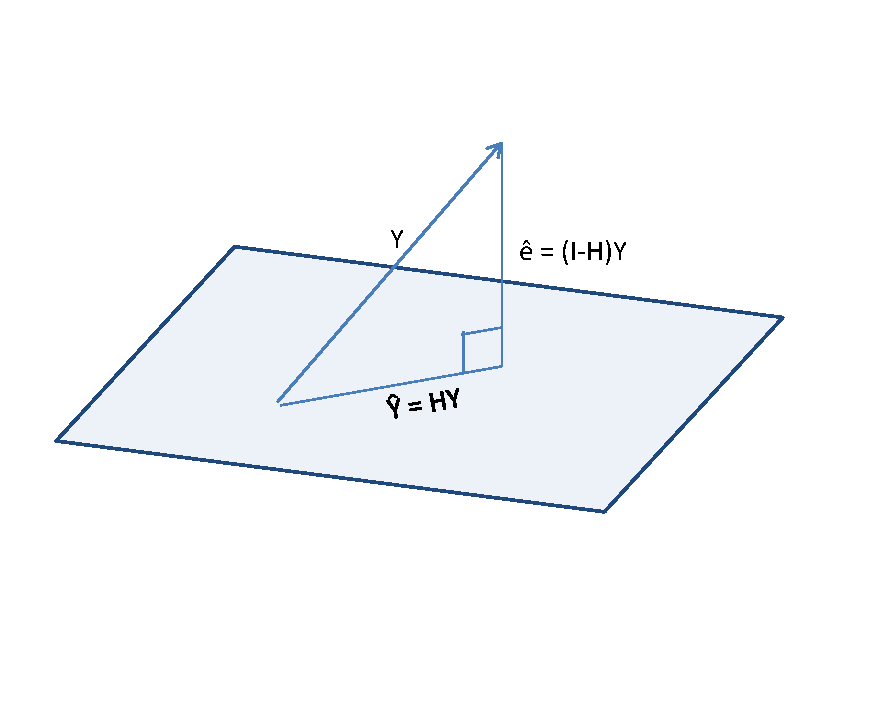
\includegraphics[scale = 0.35]{Chap6-InferenceRLM/Figures/geometrie}
	\caption{Illustration de l'analyse de la variance généralisée}
	\label{fig:geometrie}
\end{figure}



Le théorème de Pythagore donne
$$||\boY||^2=||\boX\hbobeta||^2+||\boY-\boX\hbobeta||^2,$$
o\`u $||\cdot||$ représente la norme (longueur) du vecteur.

Ainsi on retrouve la décomposition:
\begin{eqnarray*}
\boY'\boY&=&(\boX\hbobeta)'\boX\hbobeta+(\boY-\boX\hbobeta)'(\boY-\boX\hbobeta)\\
\Rightarrow\boY'\boY-n\bar{Y}^2&=&\hbobeta'\boX'\boX\hbobeta
+(\boY-\boX\hbobeta)'(\boY-\boX\hbobeta)-n\bar{Y}^2_n\\
&=&\hbobeta'\boX'\boX\hbobeta-n\bar{Y}^2+\hboeps'\hboeps,
\end{eqnarray*}


%\textcolor{red}{Faire une petit exemple ici avant de parler de F, i.e. presenter SCtot et la division en 2 et montrer que c'est plus grand dans un des cas. Ou alors je fais ca en classe...}

On peut utiliser cette décomposition pour obtenir un tableau d'analyse de la variance comme en RLS. Le tableau \ref{table:anova} résume la table ANOVA pour la RLM.


\begin{table}[htb!]
\caption{Tableau d'analyse de la variance dans le cas de la régression linéaire multiple}\label{table:anova}
\centering
\begin{footnotesize}
\renewcommand{\arraystretch}{1.6}
\begin{tabular}{ccccc}\hline
Source & Degrés de liberté & Sommes des carrés & Carrés moyens & $F$ \\ \hline
Modèle & $ddl_1=p$ &
$SC_{reg}=\sum_{i=1}^n(\hat Y_i-\bar Y)^2$ & $CM_{reg}=SC_{reg}/ddl_1$ & $CM_{reg}/CM_{res}$\\
Erreur & $ddl_2=n-p'$ & $SC_{res}=\sum_{i=1}^n(Y_i-\hat Y_i)^2$ & $CM_{res}=SC_{res}/ddl_2$ & \\
résiduelle & & & \\
\hline Totale (corrigée) & $n-1=p+n-p'$ & $SC_{tot}=\sum_{i=1}^n(Y_i-\bar Y)^2$ & &
\end{tabular}
\end{footnotesize}
\end{table}

On peut ensuite tester l'effet global de toutes les variables exogènes, soit
\begin{eqnarray}
H_0:&~&\beta_1=\beta_2=\cdots=\beta_{p}=0\label{H0:Ftest}\\
\mbox{contre\ }H_1:&~&\mbox{au moins un des coefficients n'est pas nul.}\nonumber
\end{eqnarray}

%Sous $H_0$, le mod\`ele de régression ne devrait pas expliquer la variabilité dans les $Y_i$ et donc le ratio $SC_{reg}/SC_{res}$ devrait prendre une petite valeur. Par contre sous $H_1$, le mod\`ele de régression devrait expliquer une partie de la variabilité des $Y_i$ et donc le ratio $SC_{reg}/SC_{res}$ devrait prendre une grande valeur.

Sous $H_0$, la statistique $F$ suit une loi $\mathcal F$ de Fisher-Snedecor avec $p$ degrés de liberté au numérateur et $n-p'$ degrés de liberté au
dénominateur. On rejette donc $H_0$ au niveau $\alpha$ lorsque la statistique
$\mathcal F$ est supérieure ou égale au quantile
$F_{p,n-p';1-\alpha}$.\\


\begin{exemple}
Pour l'exemple \ref{exp_data}, on peut calculer  $SC_{res}=\hboeps'\hboeps=\hat\sigma^2 (n-p')=38,21$, $SC_{tot}=\boY'\boY-n\bar{Y}^2=904,60-20\left(\frac{120,79}{20}\right)^2=175,089$ et $SC_{reg}=SC_{tot}-SC_{res}=136,88.$ On obtient donc le tableau d'analyse de la variance suivant

\begin{table}[htb!]
\caption{Tableau d'analyse de la variance pour l'exemple \ref{exp_data}}
\centering
\begin{footnotesize}
\renewcommand{\arraystretch}{1.6}
\begin{tabular}{ccccc}\hline
Source & Degrés de liberté & Sommes des carrés & Carrés moyens & $F$ \\ \hline
Modèle & $ddl_1=2$ &
$136,88$ & $136,88/2=68,44$ & $68,44/2,247=30,46$\\
Erreur & $ddl_2=17$ & $38,21$ & $38,21/17=2,247$ & \\
résiduelle & & & \\
\hline Totale & $19$ & $175,09$ & &
\end{tabular}
\end{footnotesize}
\end{table}

Pour tester $H_0:\beta_1=\beta_2=0$, on compare $F=30,46$ au quantile $F_{p,n-p'}(1-\alpha)=F_{2,17}(0,95)=3,59$. Comme $30,46>3,59$, on rejette l'hypothèse nulle. On en conclut donc que les meurtrissures de pêche sont liées soit à la hauteur de chute, soit à la masse volumique, soit aux deux.
\end{exemple}


\newpage

\section{Test de réduction du modèle}

Il est plut\^ot rare en pratique que le test $\mathcal F$ de Fisher global ne
rejette pas l'hypoth\`ese $H_0$ donnée par (\ref{H0:Ftest})
que le modèle de régression est
totalement inutile. Cependant, on veut souvent tester si
le modèle peut être réduit. Cela revient à tester
si un sous-modèle plus simple explique une partie suffisamment
grande de la variabilité dans les $Y_i$ pour qu'il ne soit pas
nécessaire d'utiliser le modèle plus complexe. Il s'agit donc de mesurer si
la différence entre les sommes de carrés résiduels des
deux modèles est faible ou élevée.

%Le principe de la somme de carrés résiduels additionnelle permet de tester cette hypoth\`ese de fa\c{}con formelle. L'idée sous-jacente est simple: si les termes qui sont exclus du modèle plus simple expliquent une partie importante de la variabilité dans les$Y_i$, alors la variabilité due à la fluctuation aléatoire ($SC_{res}$) apparaitra beaucoup plus importante dans le mod\`ele simple que dans le modèle complet.

Cette idée se traduit mathématiquement de la manière suivante. Supposons le modèle de régression
multiple standard
$$Y_i=\beta_0+\beta_1x_{i1}+\cdots+\beta_{p}x_{ip}+\varepsilon_i.$$
On désire tester si un modèle comprenant seulement $k<p$ variables exogènes
suffit à expliquer la variabilité dans les $Y_i$. Par souci de simplicité, on suppose que les $k$ variables exog\`enes en question sont $x_1,\ldots,x_k$. Alors on veut tester
\begin{eqnarray}
H_0:~Y_i&=&\beta_0+\beta_1x_{i1}+\cdots+\beta_kx_{ik}+\varepsilon_i\label{H0:ESS}\\
H_1:~Y_i&=&\beta_0+\beta_1x_{i1}+\cdots+\beta_kx_{ik}+\beta_{k+1}x_{i,k+1}+\cdots+\beta_{p}x_{ip}
+\varepsilon_i.\nonumber
\end{eqnarray}
Le mod\`ele donné par $H_0$ est appelé mod\`ele réduit, alors que l'équation présentée
en $H_1$ se nomme mod\`ele complet.

Soit $SC_{res}^{(0)}$ la somme des carrés résiduels obtenue avec
le modèle réduit et $SC_{res}^{(1)}$ la somme des carrés résiduels obtenue avec le
modèle complet. Alors il est toujours vrai que $SC_{res}^{(1)}\le SC_{res}^{(0)}$. Cependant, sous $H_0$,
la différence entre $SC_{res}^{(0)}$ et $SC_{res}^{(1)}$ sera faible, alors que cette même
différence sera élevée sous $H_1$.

Encore une fois, on standardise le rapport
$(SC_{res}^{(0)}-SC_{res}^{(1)})/SC_{res}^{(1)}$ afin d'obtenir une statistique avec une distribution connue sous $H_0$. On obtient
\begin{equation}\label{F:ESS}
F={SC_{res}^{(0)}-SC_{res}^{(1)}\over
\Delta_{dl}\hat\sigma^2_{H_1}},
\end{equation}
où $\Delta_{dl}$ note la différence entre les degrés de liberté de
$SC_{res}^{(0)}$ et les degrés de liberté de $SC_{res}^{(1)}$. Sous l'hypothèse nulle $H_0$ donnée par
(\ref{H0:ESS}), la statistique $F$ en (\ref{F:ESS}) suit une distribution $\mathcal F$ de Fisher avec $\Delta_{dl}$ degrés de
liberté au numérateur et $n-p'$ degrés de liberté au dénominateur. On rejette donc $H_0$ au
niveau de confiance $\alpha$ lorsque $F\ge F_{\Delta_{dl},n-p'}(1-\alpha)$.

%Il est à noter que $n-p'$ réfère au nombre de degrés de liberté de $SC_{res}^{(1)}$, et que $\hat\sigma^2_{(1)}$ réfère au carré moyen résiduel sous $H_1$. Comme il arrive parfois que le \og modèle complet \fg constitue un modèle qui n'inclut pas toutes les $p$ variables exogènes, il faut ajuster la formule (\ref{F:ESS}) en conséquence. C'est pourquoi il est probablement mieux de retenir la forme à droite de la seconde égalité en(\ref{F:ESS}).

On note qu'il existe plusieurs manières de calculer $\Delta_{dl}$:
\begin{enumerate}\item
$\Delta_{dl}=dl(SC_{res}^{(0)})-dl(SC_{res}^{(1)})$;
\item $\Delta_{dl}=$(nbr de paramètres du mod\`ele $H_1$)-
(nbr de paramètres du modèle $H_0$);
\item $\Delta_{dl}=$ nbr de contraintes sur les param\`etres du mod\`ele complet pour
arriver au mod\`ele réduit.
\end{enumerate}
Ainsi, dans le cas présenté en (\ref{H0:ESS}), on aurait
\begin{enumerate}
\item $dl(SC_{res}^{(0)})=n-(k+1)=n-k-1$\\
$dl(SC_{res}^{(1)})=n-p'$\\
Donc, $\Delta_{dl}=n-k-1-n+p'=p'-k-1=p-k$.
\item Param\`etres sous $H_1$: $p'=p+1$\\
Param\`etres sous $H_0$: $k+1$\\
Donc, $\Delta_{dl}=p+1-k-1=p-k$.
\item Les contraintes pour réduire le mod\`ele $H_1$ au mod\`ele $H_0$ sont
$$\beta_{k+1}~=~0,\ldots, \beta_{p}~=~0,$$ c'est-à-dire $p-k$ égalités (contraintes) sur les param\`etres du mod\`ele complet afin d'obtenir le mod\`ele réduit. Donc $\Delta_{dl}=p-k$.
\end{enumerate}

\subsection{Cas particuliers simples}

La très grande majorité des tests d'hypothèses que nous aurons à effectuer dans ce cours
pourrons \^etre exprimés sous la forme $H_0:$ mod\`ele réduit contre $H_1:$ mod\`ele complet. Trois cas particuliers ont des noms spécifiques et méritent d'être étudiés.

\textbf{Test global de la régression}

Le $F$ de la table ANOVA présentée à la dernière section constitue en fait un test de réduction de modèle dans lequel le mod\`ele complet contient toutes les variables exogènes disponibles et le modèle réduit s'écrit simplement comme $Y_i=\beta_0+\varepsilon_i$.  Dans ce cas on peut facilement voir que la statistique $F$ donnée en (\ref{F:ESS}) est égale \`a la statistique $F$ de la table ANOVA. De plus, on déduit aussi facilement que $\Delta_{dl}=p$.

\newpage
\textbf{Tests de $F$ séquentiels}

Il s'agit de tests de réduction de modèles séquentiels pour toutes les variables du jeu de données. On commence avec le modèle nul comme modèle simple et on ajoute séquentiellement chaque variable en testant si elle permet de réduire significativement la somme des carrés résiduelle.

On présente souvent les valeurs de $F$ et valeurs de $p$ associées pour les tests de $F$ séquentiels de toutes les variables d'un jeu de données dans un seul tableau. Les résultats dépendront de l'ordre dans lequel on ajoute les variables.

\begin{remarque}
Dans certains livres et logiciels on parle dans ce cas de sommes de carrés de type I.
\end{remarque}


\textbf{Tests de $F$ ajustés}

On parle de tests de $F$ ajustés quand on teste l'effet de l'ajout de chaque variable, en tenant compte de toutes les autres variables présentes dans le modèle. On dit qu'on ajuste pour toutes les autres variables présentes dans le modèle.

Un test de $F$ ajusté pour la variable $j$ teste donc
\begin{eqnarray*}
H_0:~Y_i&=&\beta_0+\beta_1x_{i1}+\cdots+ \beta_{j-1}x_{i(j-1)} + \beta_{j+1}x_{i(j+1)}+ \beta_kx_{ik}+\varepsilon_i\\
H_1:~Y_i&=&\beta_0+\beta_1x_{i1}+\cdots+ \beta_{j-1}x_{i(j-1)} + \beta_{j}x_{ij}+ \beta_{j+1}x_{i(j+1)}+ \beta_kx_{ik}+\varepsilon_i
\end{eqnarray*}

Ici aussi on présente souvent dans un seul tableau les résultats des tests de $F$ ajustés de toutes les variables d'un jeu de données. Puisqu'on ajuste à chaque fois sur toutes les variables disponibles, les résultats ne dépendront pas de l'ordre dans lequel les variables sont testées.

\begin{remarque}
On parle parfois dans ce cas de sommes de carrés de type II.
\end{remarque}

\begin{remarque}
Dans un test de $F$ ajusté pour la variable $j$, on teste en fait $H_0 : \beta_j=0$ vs $H_1 : \beta_j \ne 0$. On peut d'ailleurs montrer que ce test est équivalent au test $t$ de l'hypothèse $H_0 : \beta_j=0$ basé sur la distribution de $\hat{\bobeta}$ et mentionné à la section \ref{sec:infbetaRLM}.
\end{remarque}

\newpage
\subsection{Point de vue géométrique}

On peut également comprendre les tests de réduction de modèle d'un point de vue géométrique. La statistique $F$ du test est alors construite en standardisant les longueurs des vecteurs appropriés en les divisant par la dimension de l'espace dans lesquels ils vivent (leurs degrés de liberté). La figure \ref{fig:geometrie_gen} montre toutes les quantités impliquées.

\begin{figure}[htb!]
	\centering
		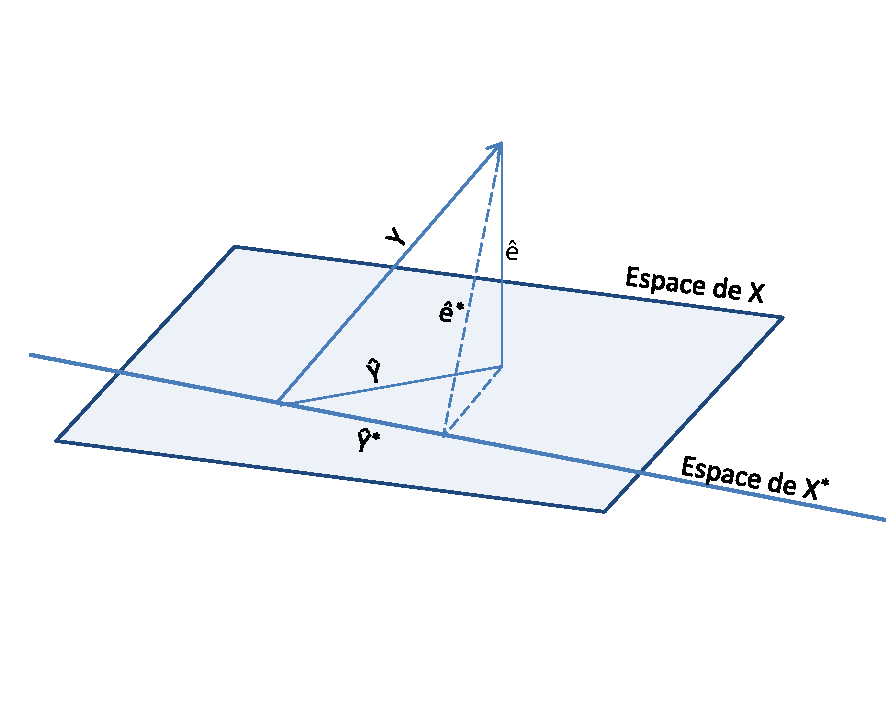
\includegraphics[scale = 0.35]{Chap6-InferenceRLM/Figures/geometrie_gen}
	\caption{Illustration de l'analyse de la variance généralisée}
	\label{fig:geometrie_gen}
\end{figure}

\begin{itemize}
\item[$\bullet$] Le plan Espace de $X$ est l'espace colonne de la matrice d'incidence sous $H_1$.
\item[$\bullet$] La droite Espace de $X^*$ est l'espace colonne de la matrice d'incidence sous $H_0$.
\item[$\bullet$] Le vecteur $\hY$ est $\boX\hbobeta$ sous le modèle complet et se situe dans un espace de dimension $p'$. Ce vecteur constitue la projection orthogonale du vecteur
$\boY$ sur le plan nommé Espace de $X$.
\item[$\bullet$] Le vecteur $\boeps$ est constitué des résidus sous le modèle complet et vit dans un
espace de dimension $n-p'$.
\item[$\bullet$] Le vecteur $\hY^*$ représente le vecteur $\boX\hbobeta$ sous le modèle réduit et évolue dans un espace de dimension $p'-\Delta_{dl}$. Ce vecteur est la projection
orthogonale du vecteur $\boY$ sur la droite Espace de $X$.
\item[$\bullet$] Le vecteur $\boeps^*$ est formé des résidus sous le modèle réduit et
vit dans un espace de dimension $n-p'+\Delta_{dl}$.
\end{itemize}

Le vecteur égal à la différence entre les vecteurs de résidus des
deux mod\`eles est important. Notons $C$ sa longueur. $C^2$ est donc la différence entre les sommes
de carrés résiduels. Ce vecteur vit dans un espace de
dimension $\Delta_{dl}$. La statistique du test $F$ du principe de
somme de carrés résiduels additionnelle est tout simplement
égale \`a $(C^2/\Delta_{dl})/(B^2/(n-p'))$ où $B$ dénote la longueur du vecteur des résidus sous le modèle complet.

\section{Test d'une hypoth\`ese linéaire générale}
\label{sec:hyplingen}

Plusieurs tests en régression linéaire peuvent être exprimés comme une liste de contraintes linéaires sur les valeurs des param\`etres. Soit $\bo{C}$, une matrice de dimension
$r\times p'$, et $\bo{d}$, un vecteur de dimension $r\times1$. Un test d'hypoth\`ese linéaire
générale s'écrit comme
\begin{eqnarray}\label{H0:lingen}
H_0:~\bo{C}\bobeta&=&\bo{d}\\
\mbox{contre\ }H_1:~\bo{C}\bobeta&\neq&\bo{d}.\nonumber
\end{eqnarray}
On peut ré-écrire ce test d'hypoth\`ese sous la forme d'un mod\`ele réduit et d'un mod\`ele
complet de la manière suivante :
\begin{eqnarray*}
H_0:~\boY&=&\bo{Z}\bo{\alpha}+\boeps\\
\mbox{vs\ \ }H_1:~\boY&=&\boX\bobeta+\boeps,
\end{eqnarray*}
où l'équation en $H_0$ est obtenue en (i) résolvant le système d'équations
$\bo{C}\bobeta=\bo{d}$ pour $\bobeta$ et (ii) en substituant la solution trouvée en (i)
dans le modèle $\boY=\boX\bobeta+\boeps$.

%Puisque le test d'une hypothèse linéaire générale est équivalent à tester un modèle réduit contre un mod\`ele complet, on peut utiliser le principe de somme des carrés résiduels additionnelle.
Il est possible de
montrer \citep[voir par e.g.][pp. 44--45 et pp. 60--64]{Sen_Sri:90} que
$$SC_{res}^{(0)}-SC_{res}^{(1)}=(\bo{C}\hbobeta-\bo{d})'[\bo{C}(\boX'\boX)^{-1}\bo{C}']^{-1}(\bo{C}
\hbobeta-\bo{d}).$$
Notez que $\sigma^2[\bo{C}(\boX'\boX)^{-1}\bo{C}']$ est la variance de $\bo{C}\hbobeta-\bo{d}$. Donc
la différence des sommes de carrés résiduels peut \^etre vue comme la longueur du vecteur
qui sépare $\bo{C}\hbobeta$ et $\bo{d}$, standardisée par sa variance. Si la distance entre
$\bo{C}\hbobeta$ et $\bo{d}$ est faible, alors $H_0$ constitue une hypothèse raisonnable, $SC_{res}^{(0)}-
SC_{res}^{(1)}$ prend une petite valeur et on ne rejette donc pas $H_0$. Si $H_0$ n'est pas réaliste, alors
$\bo{C}\hbobeta$ sera éloignée de $\bo{d}$, $SC_{res}^{(0)}-SC_{res}^{(1)}$ prendra une grande valeur
et on rejettera l'hypothèse nulle $H_0$.

On peut maintenant construire la statistique $F$ en utilisant l'équation (\ref{F:ESS}):
\begin{equation*}\label{F:lingen}
F={(\bo{C}\hbobeta-\bo{d})'[\bo{C}(\boX'\boX)^{-1}\bo{C}']^{-1}(\bo{C}\hbobeta-\bo{d})/r\over
SC^{(1)}_{res}/(n-p')}={
(\bo{C}\hbobeta-\bo{d})'[\bo{C}(\boX'\boX)^{-1}\bo{C}']^{-1}(\bo{C}\hbobeta-\bo{d})\over
r\hat\sigma^2_{H_1}},
\end{equation*}
où $r$ note le nombre de lignes de la matrice $\bo{C}$.
Le fait que $\Delta_{dl}=r$ dans ce cas est facile \`a comprendre si on utilise la troisième manière de le calculer, soit le nombre de contraintes sur les param\`etres du mod\`ele complet pour
obtenir le mod\`ele réduit. Sous l'hypothèse $H_0$, $F$ suit une loi de Fisher $\mathcal{F}_{r,n-p'}.$


%\begin{remarque}\label{rem:saslingen}
%Dans l'aide de SAS, on utilise la notation $\bo{L}\beta=\bo{c}$ plut\^ot que
%la notation $\bo{C}\bobeta=\bo{d}$ qui est utilisée par plusieurs livres.
%L'aide de SAS utilise aussi $b$ pour dénoter
%l'estimateur de $\bobeta$ plut\^ot que $\hbobeta$.
%\end{remarque}




\addtocontents{toc}{\protect\pagebreak}

\chapter{Variables catégoriques et interactions}
\label{sec:CategoriquesInteractions}

Une grande différence quand on utilise un modèle de RLM au lieu de la RLS, c'est qu'on peut créer des modèles plus complexes. On verra ici deux façons pour ce faire, soit inclure des variables catégoriques et inclure des interactions.

\section{Variables exogènes catégoriques}

Jusqu'à maintenant, nous n'avons considéré que des variables
exogènes continues. Il arrive pourtant souvent en pratique que
les variables exogènes ne puissent prendre des valeurs que dans
un ensemble de valeurs possibles, et que ces valeurs n'impliquent
pas un ordre entre les mesures. Quelques exemples:
\begin{eqnarray*}
x_{1i}&=&\left\{\begin{array}{ll} H, & \mbox{si $i$ est un homme}\\
F, & \mbox{si $i$ est une femme}\end{array}\right.\\
x_{1i}&=&\left\{\begin{array}{ll} 1, & \mbox{si $i$ est une ville}\\
-1, & \mbox{si $i$ est un village}\end{array}\right.\\
x_{1i}&=&\left\{\begin{array}{ll}1, & \mbox{si $i$ est à ON}\\
0, & \mbox{si $i$ est à OFF}\end{array}\right.\\
\end{eqnarray*}

On peut simplement ajouter une variable catégorique linéairement dans le modèle de RLM. La valeur de cette variable modifiera l'ordonnée à l'origine de la régression. Il faut toutefois faire attention à la façon avec laquelle on code les variables catégoriques pour s'assurer que le modèle soit facile à interpréter.

\newpage
\textbf{Variable dichotomique}

Dans le cas d'une variable dichotomique, il est toujours plus prudent de coder $x_i$ sous la forme d'une variable indicatrice, c'est-à-dire sous la forme
$$x_i=\left\{\begin{array}{ll} 1, & \mbox{si ...}\\
0, & \mbox{sinon}\end{array}\right.$$

Si ce type de codage n'est pas utilisé, alors les $\beta$ peuvent \^etre difficiles à
interpréter.

Par exemple si
$$x_{i}=\left\{\begin{array}{ll}-5, & \mbox{si $i$ est un homme}\\
5, & \mbox{si $i$ est une femme}\end{array}\right.$$
Alors le modèle $Y_i=\beta_0+\beta_1 x_i+\varepsilon_i$ nous donne
\begin{eqnarray*}
\esp[Y_i|\mbox{$i$ est un homme}]&=&\beta_0-5\beta_1\\
\esp[Y_i|\mbox{$i$ est une femme}]&=&\beta_0+5\beta_1
\end{eqnarray*}
On a donc que $\beta_0$ est la moyenne des espérances de $Y$ pour les hommes et les femmes, et $\beta_1$ représente 0.1 fois la différence entre la valeur moyenne de $Y$ pour les hommes et celle pour les femmes.

Si on prend plutôt
$$x_{i}=\left\{\begin{array}{ll}1, & \mbox{si $i$ est un homme}\\
0, & \mbox{si $i$ est une femme}\end{array}\right.$$ alors on a
\begin{eqnarray*}
\esp[Y_i|\mbox{$i$ est un homme}]&=&\beta_0+\beta_1\\
\esp[Y_i|\mbox{$i$ est une femme}]&=&\beta_0
\end{eqnarray*}
et maintenant $\beta_0$ est simplement la valeur moyenne de $Y$ pour les femmes et  $\beta_1$ représente exactement la différence entre la valeur moyenne de $Y$ pour les hommes et celle pour les femmes.

Un autre codage souvent utilisé durant la collecte de données est de la forme

$$x_{i}=\left\{\begin{array}{ll}1, & \mbox{si $i$ est un homme}\\
2, & \mbox{si $i$ est une femme}\end{array}\right.$$

Dans ce cas, $\beta_1$ s'interprète de la même façon qu'avec la variable indicatrice, mais $\beta_0$ est plus complexe à interpréter.

\textbf{Variable polytomique}

Si $x$ est une variable polytomique, c'est-à-dire que $x_i$ peut
prendre une parmi $C\ge2$ valeurs possibles, la fa\c{c}on prudente
de procéder est de définir $C-1$ variables indicatrices.
Ainsi,
si $$x_{1i}=\left\{\begin{array}{ll} 1, & \mbox{si $i$ est bleu}\\
2, & \mbox{si $i$ est rouge}\\ 3, & \mbox{si $i$ est jaune}\\ 4, &
\mbox{si $i$ est vert}\end{array}\right.$$ alors on définit
\begin{eqnarray*}
x_{Bi}&=&\left\{\begin{array}{ll}1, & \mbox{si $i$ est bleu}\\ 0,
& \mbox{sinon}\end{array}\right.\ \ \
x_{Ri}=\left\{\begin{array}{ll}1, & \mbox{si
$i$ est rouge}\\ 0, & \mbox{sinon}\end{array}\right.\\
x_{Ji}&=&\left\{\begin{array}{ll}1, & \mbox{si $i$ est jaune}\\
0, & \mbox{sinon}\end{array}\right.\end{eqnarray*} Dans ce cas
\begin{eqnarray*}
x_{1i}=\mbox{bleu}&\Rightarrow&(x_{Bi},x_{Ri},x_{Ji})=(1,0,0)\\
x_{1i}=\mbox{rouge}&\Rightarrow&(x_{Bi},x_{Ri},x_{Ji})=(0,1,0)\\
x_{1i}=\mbox{jaune}&\Rightarrow&(x_{Bi},x_{Ri},x_{Ji})=(0,0,1)\\
x_{1i}=\mbox{vert}&\Rightarrow&(x_{Bi},x_{Ri},x_{Ji})=(0,0,0)
\end{eqnarray*}
Ainsi, si
$Y_i=\beta_0+\beta_{B}x_{Bi}+\beta_Rx_{Ri}+\beta_Jx_{Ji}+\varepsilon_i$,
\begin{eqnarray*}
\esp[Y_i|\mbox{$i$ est bleu}]&=&\beta_0+\beta_B\\
\esp[Y_i|\mbox{$i$ est rouge}]&=&\beta_0+\beta_R\\
\esp[Y_i|\mbox{$i$ est jaune}]&=&\beta_0+\beta_J\\
\esp[Y_i|\mbox{$i$ est vert}]&=&\beta_0.
\end{eqnarray*}


\begin{remarque}
Si une variable exogène ne prend que très peu de valeurs différentes, il est important de déterminer s'il s'agit d'une variable continue pour laquelle on a peu de mesures ou s'il
s'agit d'une variable polytomique. Selon la façon avec laquelle la variable est incluse dans le modèle, l'interprétation sera différente, ainsi que l'information qu'on pourra retirer du modèle.
\end{remarque}

\newpage
\begin{exemple}
\label{eg:lot}
Soit $x_{1i}$, le numéro de lot du produit $i$, $x_{2i}$, la
concentration de sel dans le produit $i$ et $Y_i$, l'indice de
qualité du produit $i$. Les variables $Y_i$ et $x_{2i}$ sont des
variables continues, alors que $x_{1i}$ est un variable
polytomique prenant une des valeurs $\{1,2,3,4\}$.

On ajuste le modèle
$$Y_i=\beta_0+\beta_{11}x_{11i}+\beta_{12}x_{12i}+\beta_{13}x_{13i}+\beta_2x_{2i}
+\varepsilon_i,$$ o\`u
\begin{eqnarray*}
x_{11i}&=&\left\{\begin{array}{ll} 1, & x_{1i}=1\\
0, & x_{1i}\neq1\end{array}\right. \ \ \
x_{12i}=\left\{\begin{array}{ll} 1, & x_{1i}=2\\
0, & x_{1i}\neq2\end{array}\right. \\
x_{13i}&=&\left\{\begin{array}{ll} 1, & x_{1i}=3\\
0, & x_{1i}\neq3.\end{array}\right.\end{eqnarray*}

La figure \ref{figex81} illustre graphiquement ce modèle. Notez qu'on suppose dans la figure que tous les coefficients sont positifs, mais ce n'est absolument pas nécessaire en pratique.

\begin{figure}[htb!]
\begin{center}
\centerline{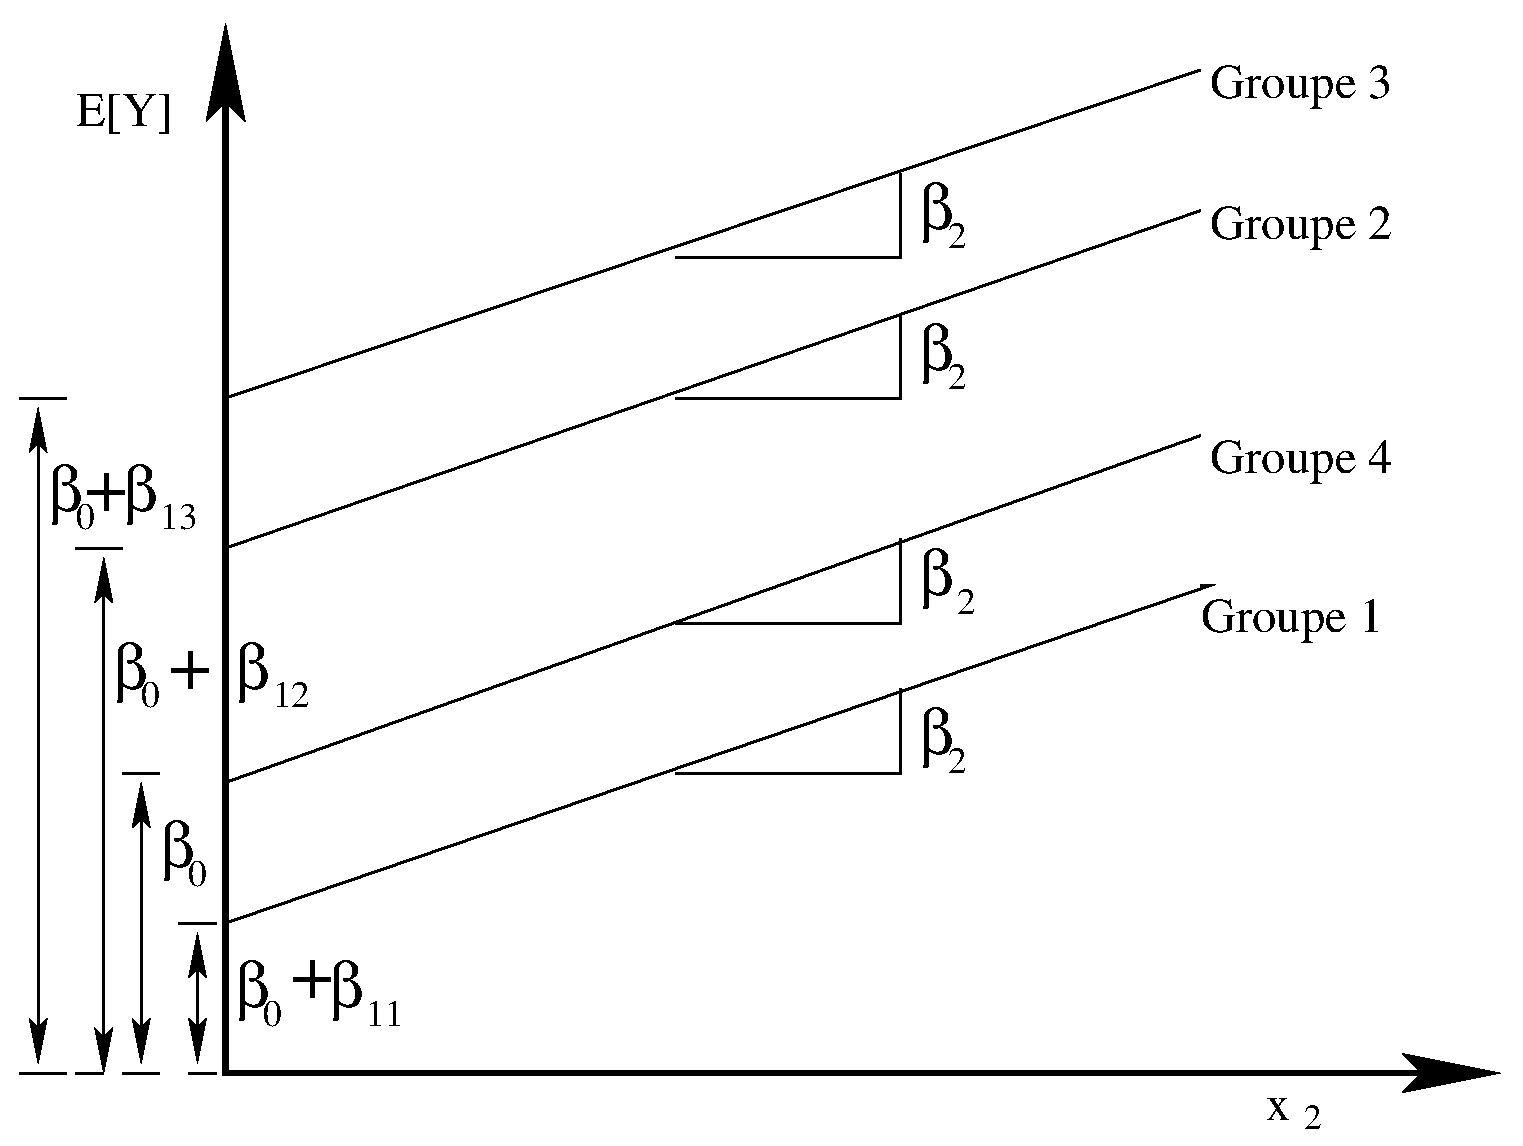
\includegraphics[height=3.5in,angle=0]{Chap7-CategoriquesInteractions/Figures/eyvsx2.eps}}
\caption[Espérance de la variable endogène $Y$ en fonction de
la variable exogène $x_2$ pour chacun des groupes 1 à 4. ]{Espérance de la variable endogène $Y$ en fonction de
la variable exogène $x_2$ pour chacun des groupes 1 à 4. Comme on
peut le voir, les $\beta_0$ et $\beta_{1j}$ déterminent les
ordonnées à l'origine, tandis que $\beta_2$ détermine la
pente des droites de régression.}\label{figex81}
\end{center}
\end{figure}
\end{exemple}


\subsection{Inférence avec des variables catégoriques}

On peut en général faire de l'inférence sur les coefficients des variables indicatrices exactement comme pour les coefficients des variables continues.

\textbf{Tester l'utilité globale d'une variable polytomique}

Il faut toutefois faire attention si on veut tester si une variable polytomique possède un effet significatif
sur la valeur moyenne de la variable endogène. On doit alors tester si
plusieurs coefficients sont simultanément égaux à zéro à
l'aide d'un test $F$ de réduction de modèle. En général, pour tester si une variable polytomique prenant
$C$ valeurs possibles a un effet significatif, il faut tester si
$C-1$ coefficients sont simultanément égaux à zéro.

\begin{exemple}
Supposons que dans le modèle de l'exemple \ref{eg:lot} on souhaite tester si le groupe
d'o\`u provient l'item $i$ a un effet sur la variable dépendante. Il faut alors tester $H_0:\beta_{11}=\beta_{12}=\beta_{13}=0$. Notez que ceci revient à tester si la droite de régression est la m\^eme pour les 4 groupes, c'est-à-dire que sur la figure
\ref{figex81}, les 4 lignes sont superposées.
\end{exemple}

\textbf{Tester une hypothèse plus complexe sur les différents niveaux d'une variable}


Notons aussi que plusieurs hypothèses intéressantes dans un modèle avec variables polytomiques peuvent \^etre vues comme des hypothèses linéaires sur les $\beta$, ce qui nous permet d'utiliser nos résultats de la section \ref{sec:hyplingen}.

\begin{exemple}
Toujours pour le modèle de l'exemple \ref{eg:lot}, supposons qu'on veut tester que la valeur moyenne de $Y_i$ est la m\^eme pour les lots 1 et 3. Ceci revient à tester si $\beta_{11} = \beta_{13}$. On peut donc utiliser un test d'hypothèse linéaire générale avec $$\bo{C} = (0,1,0,-1,0).$$
On pourrait aussi vouloir tester si on peut diviser les lots en deux : les lots 1 et 3 ayant la même moyenne, et les lots 2 et 4 ayant la même moyenne. Ici encore, c'est un test d'hypothèse linéaire générale, mais avec deux contraintes simultanées. La matrice C appropriée est alors:

$$ \bo{C}  =
\begin{bmatrix}
    0 & 1 & 0 & -1 & 0 \\
    0 & 0 & 1 & 0 & 0
\end{bmatrix}.
$$
\end{exemple}




\section{Interactions}

Une interaction entre deux variables exogènes $x_{1i}$ et $x_{2i}$ est un terme de la forme $$\beta_{12}x_{1i}x_{2i}.$$ On inclut une interaction dans un modèle lorsque l'effet d'une des variables sur la moyenne de $Y$ dépend de la valeur d'une autre variable. En effet, supposons le modèle
\vspace{-0.05in}
\begin{equation*}
Y_i=\beta_0+\beta_1x_{1i}+\beta_2x_{2i}+\beta_{12}x_{1i}x_{2i}+
\varepsilon_i.
\end{equation*}
On a alors
\vspace{-0.05in}
\begin{eqnarray}
\esp[Y_i|x_{1i}+1]&=&\beta_0+\beta_1(x_{1i}+1)+\beta_2x_{2i}+\beta_{12}(x_{1i}+1)x_{2i}\label{eq1}\\
\esp[Y_i|x_{1i}]&=&\beta_0+\beta_1x_{1i}+\beta_2x_{2i}+\beta_{12}x_{1i}x_{2i}.\label{eq2}
\end{eqnarray}
L'effet d'une augmentation d'une unité de $x_{1i}$ sur $\esp[Y_i]$ est
$\beta_1+\beta_{12}x_{2i}$, c'est-à-dire que l'effet d'une augmentation
de $x_{1i}$ d'une unité sur $\esp[Y_i]$ \textbf{dépend de la valeur
de $x_{2i}$}.

%Alors que l'inclusion d'une variable catégorique dans le modèle modifie l'ordonnée à l'origine, l'inclusion d'une interaction modifie plutôt la pente de la droite ou de l'hyperplan.

\begin{exemple}\label{ex83}
Soit $x_{1i}$ une variable polytomique pouvant prendre les valeurs
$\{1,2,3\}$ et soient $x_{11i}$ l'indicatrice que $x_{1i}=1$ et
$x_{12i}$ l'indicatrice que $x_{1i}=2$. Le modèle
$$Y_i=\beta_0+\beta_{11}x_{11i}+\beta_{12}x_{12i}+\beta_2x_{2i}
+\beta_{112}x_{11i}x_{2i}+\beta_{122}x_{12i}x_{2i}+\varepsilon_i.$$
est illustré à la figure \ref{figex83}.
%Les $\beta_0$ et $\beta_{1ji}$ déterminent les ordonnées à l'origine, tandis que $\beta_2$ et $\beta_{1j2}$ déterminent les pentes des droites de régression.
\begin{figure}[h!]
\begin{center}
\centerline{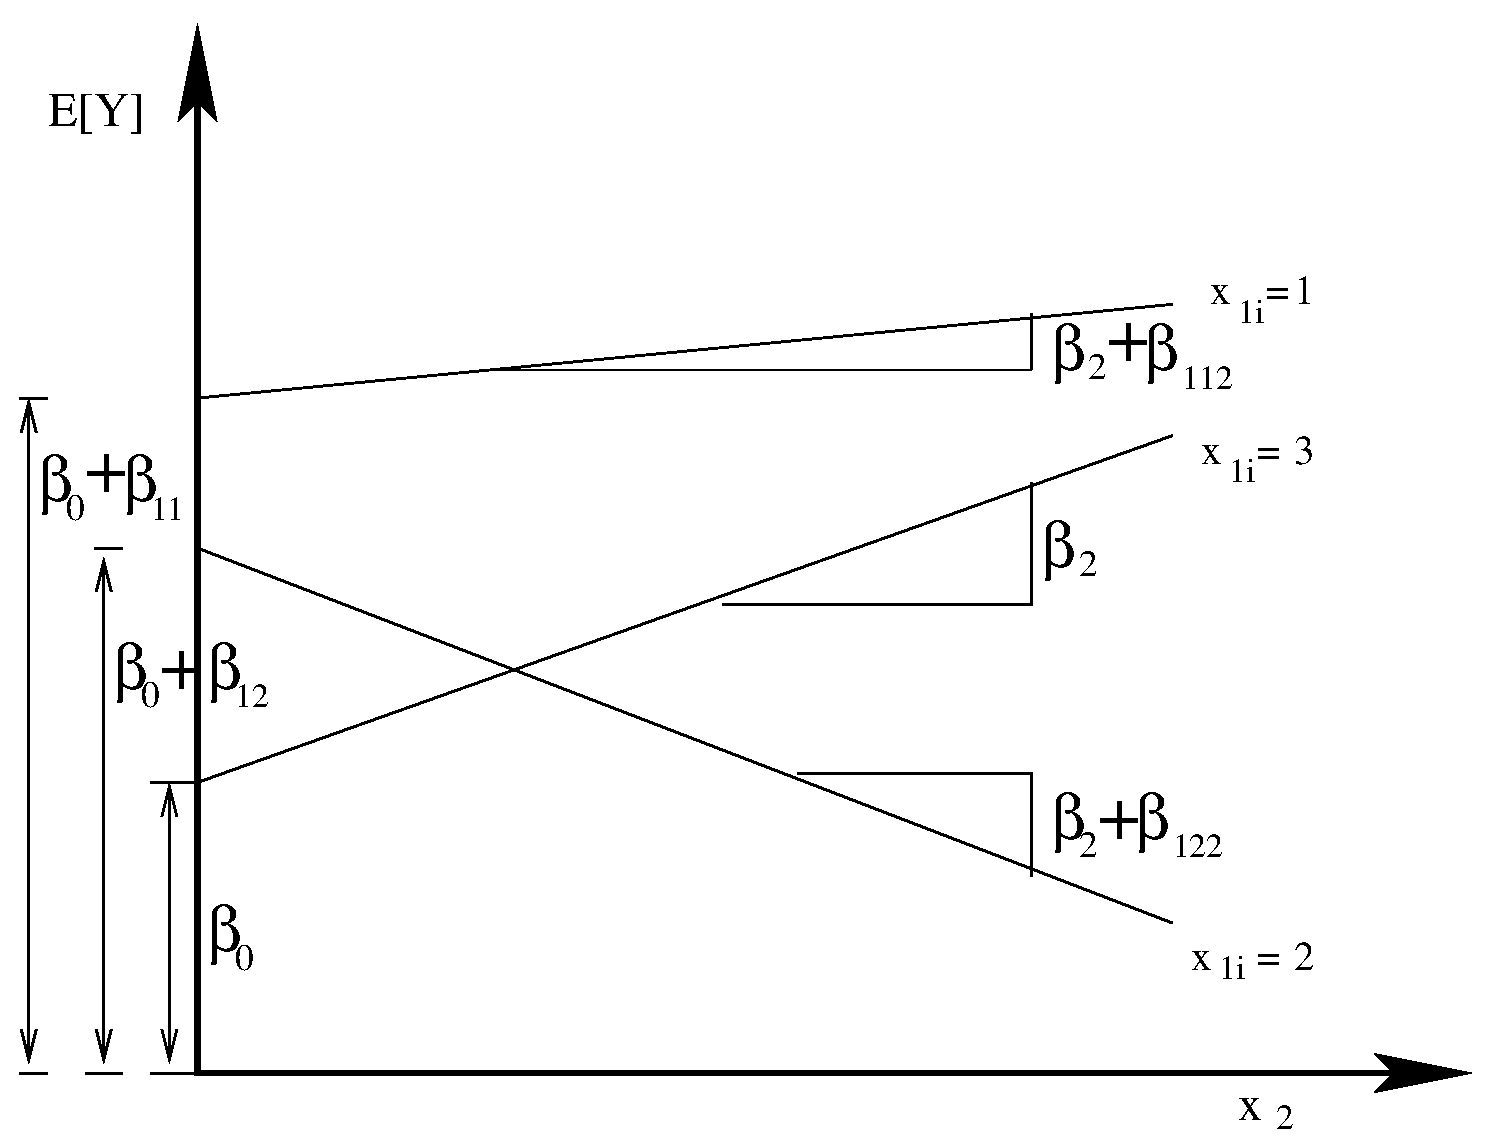
\includegraphics[scale = 0.35]{Chap7-CategoriquesInteractions/Figures/eyvsx2b.eps}}
\caption{Espérance de la variable endogène $Y$ en fonction de
la variable exogène $x_2$ pour chacune des valeurs de $x_{1i}$.
}\label{figex83}
\end{center}\end{figure}
\end{exemple}



L'exemple 7.4 illustre une interaction entre une variable catégorique et une variable continue, ce qui s'illustre aisément. On peut également inclure une interaction entre deux variables catégoriques, ce qui crée en quelque sorte une nouvelle variable catégorique avec plus de catégories. Ou entre deux variables continues, ce qui implique une pente de régression pour une première variable qui diffère pour chaque valeur d'une autre variable.

De plus, les termes d'interaction ne sont pas limités à seulement deux variables. En effet, si nous mesurons 4 variables $x_1,\ldots,x_4$
il se pourrait que le modèle approprié soit
\begin{eqnarray*}
Y_i&=&\beta_0+\beta_1x_{1i}+\beta_2x_{2i}+\beta_3x_{3i}+\beta_4x_{4i}+
\beta_{12}x_{1i}x_{2i}+\beta_{13}x_{1i}x_{3i}\\
&\ &\ \ \ +\beta_{14}x_{1i}x_{4i}+\beta_{23}x_{2i}x_{3i}+
\beta_{24}x_{2i}x_{4i}+\beta_{34}x_{3i}x_{4i}\\
&\ &\ \ \ +\beta_{123}
x_{1i}x_{2i}x_{3i}+\cdots+\beta_{1234}x_{1i}x_{2i}x_{3i}x_{4i}
+\varepsilon_i.\end{eqnarray*} Mais à moins de posséder vraiment beaucoup
de données, les interactions impliquant plus de deux variables
sont rarement utilisées. Elles sont en outre plus complexes à interpréter.


\subsubsection*{Test de linéarité}

Pour tester si un modèle est adéquat, on peut y ajouter des
termes d'interaction et tester si ces termes sont significatifs.
\begin{exemple}
Soit le modèle
$$Y_i=\beta_0+\beta_1x_{1i}+\beta_2x_{2i}+\varepsilon_i.$$ Nous pouvons tester si
$H_0:\ \beta_{12}=0$ contre $H_1:\ \beta_{12}\neq0$ à partir du
modèle
$$Y_i=\beta_0+\beta_1x_{1i}+\beta_2x_{2i}+\beta_{12}x_{1i}x_{2i}+\varepsilon_i.$$
Si nous ne rejetons pas $H_0$, alors le modèle sans
l'interaction est adéquat. Si nous rejetons $H_0$, alors le
modèle sans interaction n'est pas adéquat.\\
\end{exemple}

\begin{remarque}
Un cas particulier d'interaction est si on inclut une interaction entre une variable $x_j$ et elle-même, ce qui crée un terme de la forme $x_j^2$ dans l'équation de régression. Ce peut être utile si la relation entre les variables est quadratique plutôt que linéaire. On y reviendra à la section \ref{sec:regpoly}.
\end{remarque} 
%\addtocontents{toc}{\protect\pagebreak}
\chapter{Choix de modèle pour la RLM}
\label{sec:ChoixModeleRLM}

Comme pour la RLS, il est important lors du choix de modèle de s'assurer que les postulats sont bien respectés. Une autre difficulté de la RLM est qu'il faut choisir les variables à inclure dans le modèle parmi toutes celles à notre disposition. Nous abordons ces deux étapes dans ce chapitre.

\section{Vérification des postulats et transformations}

L'analyse des résidus pour la RLM est très similaire à celle des résidus pour la RLS. Nous révisons ici brièvement les notions du chapitre \ref{sec:ChoixModeleRLS}, et introduisons quelques nouvelles procédures.

\subsection{Les résidus}

Comme pour la RLS, le résidu est l'outil de base pour la vérification des postulats. On a déjà vu à la section \ref{sec:distYhatEps} que $\hboeps=\boY-\hY=(\boI_n-\boH)\boY$ et que
\begin{eqnarray*}
	\hboeps \sim \N_n(0, \sigma^2(\boI_n-\boH)).
\end{eqnarray*}

Tout comme pour la RLS, les résidus suivent une loi normale de moyenne $\bm{0}$, mais ne sont pas indépendants et n'ont pas des variances homogènes.

Les résidus standardisés et studentisés sont définis exactement comme pour la RLS:

$$r_i = \dfrac{\hat\varepsilon_i}{\sqrt{\hat\sigma^2(1-h_{ii})}}
\hspace{1cm}
t_i={\hat\varepsilon_i\over \hat{\sigma}_{(i)} \sqrt{1-h_{ii}}}$$


%La plupart des graphiques du Chapitre 2 sont toujours très utiles pour la validation des postulats du modèle et s'interprètent de la m\^eme fa\c{}con qu'auparavant.  Nous traiterons dans les sections suivantes quelques \'etapes de validation d'un modèle de r\'egression lin\'eaire multiple.

\subsection{Vérification de la linéarité}

On peut utiliser les mêmes graphiques que pour la RLS. On doit notamment observer le graphique de  $\hboeps$ \textit{versus} $x_j$ pour toutes les variables explicatives. On pourra alors identifier la ou les variables pour lesquelles la relation avec $Y$ n'est pas linéaire, et corriger le problème par une transformation appropriée.

% Ces graphiques devraient ne montrer aucune tendance, avec les résidus symétriques autour de zéro en ordonnée et une variabilité qui ne varie pas beaucoup en fonction de la valeur de $x_ji$. \vspace{1mm}

Toutefois, \textbf{les graphiques à variable ajoutée} sont mieux adaptés au contexte de la régression multiple pour détecter le manque de linéarité. Un graphique à variable ajoutée est un nuage de points de $\hboeps_{\boY|\boX_{-j}}$ vs $\hboeps_{x_j|\boX_{-j}}$. Ici $\hboeps_{\boY|\boX_{-j}}$ représente le vecteur des
résidus obtenu en régressant $\boY$ sur toutes les variables
exogènes du modèle \textbf{excepté} $x_j$. Il s'agit donc de la partie des $Y_i$ qui n'est pas expliquée par l'ensemble des variables exogènes, sauf la variable d'intérêt.  On veut ensuite savoir si ajouter la variable $x_j$ permet d'expliquer davantage les $Y_i$.  On pourrait tout simplement regarder la relation entre $x_j$ et $\hboeps_{\boY|\boX_{-j}}$, mais puisque $x_j$ peut lui-même être expliqué par les autres variables exogènes, il faut être un peu plus rusé. On utilise donc $\hboeps_{x_j|\boX_{-j}}$, soit le vecteur des résidus de la régression avec $x_j$ comme variable endogène et toutes les variables explicatives sauf $x_j$ comme variables exogènes. On l'obtient en ajustant le modèle suivant:
\begin{equation*}
  x_{ij} = \delta_0+\delta_1x_{i1}+...+\delta{p}x_{ip} +\varepsilon_{i\,[x_j|\boX_{-j}]}.
\end{equation*}
Plus les résidus de cette régression sont grands, plus $x_j$ ajoute de l'information importante au modèle.

Le nuage de points de $\hboeps_{\boY|\boX_{-j}}$ vs $\hboeps_{x_j|\boX_{-j}}$ tombera dans un des trois cas suivants:
\begin{itemize}
\item Si $x_j$ est vraiment une variable qui entre linéairement dans le modèle, \\
 le graphique devrait donner une droite de pente $\beta_j$ passant par l'origine.
\item  Si $x_j$ est \og inutile \fg, \\
le graphique devrait ressembler à un graphique de
résidus ordinaires.
\item  Si $x_j$ est utile mais entre dans le modèle de fa\c{}con non linéaire,\\
 le graphique devrait avoir l'allure d'une courbe plut\^ot que d'une droite.  On pourra donc détecter le manque de linéarité en $x_j$ de la moyenne de $\boY$.
\end{itemize}

\vspace{0.05 in}
Dans certains cas, il est également possible de tester la linéarité d'un modèle à l'aide d'un test de manque d'ajustement. Nous présentons celui-ci à la section \ref{sec:testAjustement}.

\newpage

\subsection{Homogénéité des variances}

On teste l'homogénéité des variances avec le graphique $r_i$ vs $\hat{Y}_i$ comme pour la RLS. S'il y a un problème, on tentera souvent de le régler en transformant la variable endogène.

Notons également qu'il existe un test formel de l'homogénéité des variances, soit le test de \citet{Whi:1980}. La statistique du test de White s'exprime comme suit
$$\chi^2_{\text{White}} = nR^2 \sim \chi^2_{p(p+3)/2}$$
o\`u $R^2$ est le coefficient de détermination ($R^2$) de la régression de $\hat\varepsilon_i^2$ sur toutes les variables explicatives $x_j$, de m\^eme que sur tous les produits croisés entre ces variables, incluant le carré de chacune des variables. On rejette l'hypothèse d'homogénéité des variances au seuil
$\alpha$ lorsque $\chi^2_{\text{White}}>\chi^2_{p(p+3)/2;1-\alpha}$.

\subsection{Normalité des erreurs}

Les mêmes outils que pour la RLS peuvent être utilisés pour tester la normalité des erreurs. Quand le postulat de normalité n'est pas rencontré, il peut \^etre souhaitable  d'utiliser la technique de transformation de Box-Cox (voir section \ref{sec:LaTechniqueDeBoxCox}) pour déterminer la meilleure transformation de la variable endogène.

Il vaut la peine de noter que le test de Shapiro-Wilk est très puissant et que
pour de gros échantillons, il rejettera très souvent la
normalité. Comme les seuils des tests $t$ de Student et $F$ de Fisher ne sont pas
sérieusement affectés si la distribution des résidus est
près de la normalité sans l'atteindre exactement, alors il est
toujours bon d'accompagner le test de normalité d'un diagramme quantile-quantile pour s'assurer que la non-normalité est vraiment sérieuse.

\subsection{Indépendance des erreurs}

On vérifie l'indépendance des erreurs exactement de la même façon que pour la RLS. Si les données sont chronologiques, on peut utiliser un graphique des résidus versus le temps. Sinon, il faut se fier à la description de la collecte de données.

\newpage
\subsection{Test pour manque d'ajustement (lack-of-fit)}
\label{sec:testAjustement}

Ce test permet de vérifier si le modèle proposé s'ajuste bien
aux données. Il constitue un bon complément à l'analyse des
résidus. Toutefois, ce test ne peut être utilisé que lorsque nous avons plusieurs observations dont la (les) variable(s) exogène(s) a (ont) exactement la (les) m\^eme(s) valeur(s).

\begin{exemple}
\label{lof1}
Le tableau \ref{jeuLOF} montre un jeu de données où les observations 2 et 3, 4 et 5 et 7 et 8 ont les m\^emes combinaisons de valeurs pour leurs variables exogènes. Un test de manque d'ajustement est donc possible dans ce cas.

\begin{table}[h!]
\begin{center}
\begin{tabular}{||cccc||cccc||}\hline\hline
Obs & $Y_i$ & $x_{1}$ & $x_{2}$ & Obs & $Y_i$ & $x_{1}$
& $x_{2}$ \\ \hline\hline
 1 &  8.74 & 2 & 1 &&&& \\
 2 & 7.10 & 2 & 0 & 3 & 9.85 & 2 & 0 \\ 4 & 12.1 & 5 & 1 & 5 & 13.1 & 5 & 1 \\
 6 & 14.1 & 5 & 0 &&&& \\
 7 & 18.6 & 8 & 1 & 8 & 15.0 & 8 & 1 \\
 9 & 16.9 & 8 & 0 &&&& \\
\hline\hline
\end{tabular}\end{center}
\caption{Jeu de données pour lequel le test de manque d'ajustement s'applique.}
\label{jeuLOF}
\end{table}
\end{exemple}

Le test de manque d'ajustement se base sur le fait qu'on peut estimer $\sigma^2$ (l'erreur pure) gr\^ace à la variabilité de la variable endogène parmi les observations ayant une m\^eme combinaison de variables exogènes. On peut ainsi séparer notre somme de carrés résiduels en une partie due à l'erreur pure et une partie due au manque d'ajustement du modèle. Mathématiquement, on écrira
$$
{\underbrace{\sum_{k=1}^m\sum_{j=1}^{n_k}(Y_{kj}-\hat{Y}_k)^2}\atop
SC_{res}}={\underbrace{\sum_{k=1}^m\sum_{j=1}^{n_k}(Y_{kj}-\overline{Y}_k)^2}
\atop
SC_{pure}}+{\underbrace{\sum_{k=1}^mn_k(\overline{Y}_k-\hat{Y}_k)^2}
\atop SC_{ajust.}}.$$
o\`u
\begin{itemize}
\item[$\bullet$] $m$ est le nombre de combinaisons distinctes des valeurs des variables exogènes
\item[$\bullet$] $n_k$, le nombre d'observations de la $k^e$ combinaison de variables exogènes
\item[$\bullet$] $Y_{kj}$ la $j^e$ observation de la variable endogène pour la $k^e$ combinaison de variables exogènes
\item[$\bullet$] $\overline{Y}_k=\sum_jY_{kj}/{n_k}$, la valeur moyenne de la variable
endogène pour la $k^e$ combinaison de variables exogènes
\end{itemize}



%La variabilité dans les $Y_i$ peut maintenant \^etre estimée à partir des données ayant les m\^emes combinaisons pour les variables exogènes, et ce m\^eme sans modèle: $$s^2={\sum_{i=1}^m\sum_{j=1}^{n_i}(Y_{ij}-\overline{Y}_i)^2\over\sum_{n_i-1}}.$$


Si le modèle de régression est adéquat, alors $\hat{Y}_k$ sera une bonne estimation de la vraie moyenne de $Y$ pour la $k^e$ combinaison de variables exogènes. Dans ce cas, $\overline{Y}_k$ sera proche de la valeur prédite $\hat{Y}_k$ et la $SC_{ajust.}$ sera petite. On compare $SC_{ajust.}$ à $SC_{pure}$ pour tester l'adéquation du modèle.

On teste donc les hypothèses

$H_0 : E(Y_i) = \beta_0 + \beta_1 x_1 + \ldots \beta_p x_p$ \\
$H_1 : E(Y_i) \ne \beta_0 + \beta_1 x_1 + \ldots \beta_p x_p$

On procède alors à une analyse de variance, résumée au tableau \ref{tab:anovaLOF}.

\begin{table}[h!]
\centering
\begin{tabular}{|c||c|c|c|c|}\hline\
 & dl & SC & CM & $F$  \\ \hline\hline
 Manque &  $m-p'$ & $SC_{ajust.}$ &    $\frac{SC_{ajust.}}{m-p'}$  &     ${SC_{ajust.}/(m-p')\over SC_{pure}/(n-m)}$   \\
 d'ajustement & & & &  \\
 Erreur pure  & $n-m$ & $SC_{pure}$ &   $\frac{SC_{pure}}{n-m}$  & \\
 Erreur totale & $n-p'$ & $SC_{res}$ &    &  \\ \hline
\end{tabular}
\caption{Table d'ANOVA pour un test de manque d'ajustement}
\label{tab:anovaLOF}
\end{table}

On rejette $H_0$ si  $F \ge F_{m-p',n-m,\;1-\alpha}$. On peut également obtenir une valeur de $p$ en comparant notre statistique $F$ à la distribution $F_{m-p',n-m}$.

\vspace{0.05in}
\begin{exemple}
Dans les données de l'exemple \ref{lof1}, on a $m=6$ combinaisons de valeurs différentes pour $(x_{1i},x_{2i})$: $\{ (2,1),(2,0),  (5,1), (5,0), (8,1),(8,0)\}$. \\
On a par exemple $n_2=2$ observations avec $(x_{1i},x_{2i})=(2,0)$, et $\overline{Y}_2=8.475$.\\
On peut calculer les 5 autres moyennes pour obtenir $SC_{pure}$.

On ajuste également le modèle $Y_{ij}=\beta_0+\beta_1x_{1i}+\varepsilon_i$, et on obtient alors $\hat{Y}_1, \ldots, \hat{Y}_6$, ce qui permet de calculer $SC_{res}$ et $SC_{ajust.}$. On trouve:

\begin{center}
\begin{tabular}{||c||c|c|c|c|c||}\hline\hline
  & dl & SC & CM & F & $Pr>F$ \\ \hline\hline
 Manque ajustement &  3 &    1.598029 &    0.53267  &     0.1484   &
 0.9242 \\
 Erreur pure  &  3 &   10.76125 &    3.58708  & & \\
 Erreur totale &  6 &   12.3598 &   2.0599   & & \\ \hline\hline
\end{tabular}
\vspace{5mm}
\end{center}

\vspace{-0.05in}
Il ne semble pas y avoir de problème de manque d'ajustement dans notre exemple. Bien entendu, avec le très petit nombre de données observé, très peu d'hypothèses peuvent \^etre rejetées!
\end{exemple}

\newpage
\section{Importance de la sélection de variables}

Pour la RLM, la vérification des postulats n'est pas le seul élément important dans le choix du modèle. Il faut aussi sélectionner les variables à inclure dans le modèle.

En effet, il se peut que certaines variables dans notre jeu de données de soient pas associées à la variable réponse.
%On verra à la section \ref{sec:inclurevar} qu'il est important d'inclure toute les variables utiles, et seulement celles-ci.
En présence d'un grand nombre de variables exogènes, on court deux dangers: enlever une variable qui est utile pour expliquer la variable endogène, et conserver dans le modèle une variable qui n'est pas utile.

\textbf{Conserver une variable inutile}

Si on conserve trop de variables, on va augmenter inutilement la variance des estimations. Par conséquent, certains effets importants risquent d'être jugés non significatifs.

Plus précisément, supposons que le bon modèle soit:
\begin{eqnarray}
% \nonumber to remove numbering (before each equation)
Y_i &=& \beta_0+\beta_1 x_{1i}+...+\beta_k x_{ki}+ \varepsilon_i.
\label{eq:modelekvar}
\end{eqnarray}
Si on ajoute la variable $x_{k+1}$ et qu'on ajuste le modèle:
\begin{eqnarray}
% \nonumber to remove numbering (before each equation)
\label{eq:modelekplus1var}
  Y_i &=& \beta_0^*+\beta_1^* x_{1i}+...+\beta_k^* x_{ki}+ \beta_{k+1}^* x_{(k+1)i}+ \varepsilon_i
\end{eqnarray}

on obtiendra que $$\var[\hat\beta^*_j] \geq \var[\hat\beta_j],\qquad\text{pour } \;j=1,...,k.$$
De plus, la prévision faite pour $Y$ en un $\bo{x}^*$ donné sera moins précise avec le modèle superflu de l'équation \eqref{eq:modelekplus1var} qu'avec le modèle simple de l'équation \eqref{eq:modelekvar}.

\textbf{Enlever une variable utile}

À l'opposé, si on enlève trop de variables, le modèle sera biaisé. Pour illustrer le biais, prenons par exemple les deux modèles suivants exprimés sous forme matricielle :
\begin{eqnarray}
% \nonumber to remove numbering (before each equation)
  \boY &=& \boX_1\bobeta_1 + \boeps,
  \label{eq:1parametre}
  \end{eqnarray}
  \begin{eqnarray}
  \boY &=& \boX_1\bobeta_1 +\boX_2\bobeta_2 +\boeps,
  \label{eq:2parametres}
\end{eqnarray}
où $\bobeta_1$ comporte $p'=p+1$ paramètres et $\bobeta_2$ inclut $m-p'$ paramètres.

Supposons que le bon modèle soit celui de l'équation \eqref{eq:2parametres} et qu'on choisisse plutôt le modèle de l'équation \eqref{eq:1parametre}, on aura alors
\begin{eqnarray*}
% \nonumber to remove numbering (before each equation)
  \esp[\hbobeta_1] &=& (\boX_1'\boX_1)^{-1}\boX_1'\esp[\boY] \\
  &=&  (\boX_1'\boX_1)^{-1}\boX_1' (\boX_1\bobeta_1 + \boX_2\bobeta_2)\\
  &=& \bobeta_1 + (\boX_1'\boX_1)^{-1}\boX_1'\boX_2 \bobeta_2.
\end{eqnarray*}
On a donc que $\hbobeta_1$ est un estimateur biaisé.

Si l'on s'intéresse plutôt à la prévision au point $\bo{x}^* = \left[\begin{array}{cc}\bo{x}_1^*\\\bo{x}_2^*\end{array}\right]$, le modèle à $p'$ paramètres nous donnerait
\begin{eqnarray*}
% \nonumber to remove numbering (before each equation)
   \hY(\bo{x}_1^{*}) &=& \bo{x}_{1}^{*'} \hbobeta_1 \\
  \esp[\hY(\bo{x}_1^{*})] &=& \bo{x}_{1}^{*'} \esp[\hbobeta_1]  \\
     &=& \bo{x}_{1}^{*'} \{\bobeta_1 + (\boX_1'\boX_1)^{-1}\boX_1'\boX_2 \bobeta_2\}
\end{eqnarray*}
alors que le modèle à $m$ paramètres conduirait à
\begin{eqnarray*}
   \hY(\bo{x}^{*}) &=& \bo{x}_{1}^{*'} \hbobeta_1^* + \bo{x}_{2}^{*'}\hbobeta_2^* \\
  \esp[\hY(\bo{x}^{*})] &=&  \bo{x}_{1}^{*'} \bobeta_1 + \bo{x}_{2}^{*'}\bobeta_2.
\end{eqnarray*}

Le biais dans la prévision serait donc
\begin{eqnarray*}
% \nonumber to remove numbering (before each equation)
   \mbox{biais}[\hY(\bo{x}^{*})]&=&  \esp[\hY(\bo{x}_1^{*})] -\esp[\hY(\bo{x}^{*})]\\
   &=& \bo{x}_{1}^{*'} \{\bobeta_1 + (\boX_1'\boX_1)^{-1}\boX_1'\boX_2 \bobeta_2\} -  \bo{x}_{1}^{*'} \bobeta_1 - \bo{x}_{2}^{*'}\bobeta_2\\
   &=& [{\bo{x}_{1}^{*'}(\boX_1'\boX_1)^{-1}\boX_1'\boX_2}-\bo{x}_{2}^{*'}]\bobeta_2.
\end{eqnarray*}

\textbf{En somme}

En résumé, un trop grand nombre de variables mène à une variance trop grande et un trop petit nombre de variables conduit à une estimation biaisée. Il est donc important de chercher un ensemble de variables permettant d'atteindre un compromis entre ces deux critères. Pour ce faire, on a souvent recours à l'une des techniques de sélection de variables pour choisir un sous-ensemble raisonnable de variables.

\newpage

\section{Critères basés sur l'ajustement du modèle}

Pour sélectionner les bonnes variables dans le modèle, plusieurs techniques sont disponibles. Voyons d'abord quelques critères basés sur l'ajustement du modèle.

\subsection{Coefficient de détermination}

Comme pour la RLS, le coefficient de détermination est défini comme
\begin{equation}\label{R^2}
R^2={SC_{reg}\over SC_{tot}}=1-{SC_{res}\over SC_{tot}}.
\end{equation}

C'est une mesure d'ajustement du modèle facile à calculer et à interpréter, mais il est problématique pour la RLM puisque sa valeur ne peut jamais diminuer si on ajoute une variable dans le modèle, même si celle-ci est inutile.

En effet, si on ajoute un terme à un modèle de régression, $SC_{reg}$ ne peut pas diminuer. Comme $SC_{tot}$ ne dépend pas du modèle, elle reste inchangée. Donc l'ajout d'un terme au modèle se traduit forcément par un $R^2$ plus grand.
%Ainsi, si le ``vrai" modèle générant les données est $Y_i=\beta_0+\beta_1x_{i1}+\varepsilon_i$ et que l'on ajuste ce modèle ainsi que le modèle $Y_i=\beta_0+\beta_1x_{i1}+\beta_2x_{i2}+\varepsilon_i$, il est fort probable que le $R^2$ du second modèle soit supérieur à celui du ``vrai" modèle.
L'ajout de termes superflus réduit en général la précision dans les prévisions, ce qu'on souhaite éviter. Le coefficient de détermination n'est donc pas utile pour la RLM.

\subsection{Coefficient de détermination ajusté}

Il s'agit d'un coefficient de détermination qui pénalise pour l'ajout d'un trop grand nombre de variables. Plus précisément, il est défini comme :
\begin{equation}\label{R^2a}
R^2_{a}=1-{CM_{res}\over CM_{tot}}=1-{SC_{res}/(n-p')\over
SC_{tot}/(n-1)}=1-{(n-1)\hat\sigma^2\over SC_{tot}}.
\end{equation}
Avec $R^2_{a}$, l'ajout d'une variable exogène peut aussi
résulter en une diminution de la statistique.
%Tout comme
%c'était le cas pour $R^2$, la valeur maximale que peut prendre
%$R^2_{ajus}$ est 1.
Comme on peut le voir dans la dernière
égalité de l'équation (\ref{R^2a}), comparer deux
modèles sur la base de leur $R^2_{a}$ est équivalent à
comparer deux modèles sur la base de leur estimation de la
variance des termes d'erreur $\hat\sigma^2$, puisque $SC_{tot}$ et $n$ ne
dépendent pas du modèle choisi.

Notez que peu importe si on utilise $R^2$ ou $R^2_{a}$, on ne peut pas vraiment se fier sur ces statistiques pour comparer des modèles employant des transformations différentes de la variable endogène, ou un modèle avec et un modèle sans ordonnée à l'origine.


\subsection{Critère d'information d'Akaike (AIC)}

%%%%%%%%%%%%%%%%%%%%%%%%%%%%%%%%%%%%%%%%%%%%%%%%%%%%%%%%%%%%%%
% Je crois que les commandes AIC et BIC dans R comptent sigma comme un paramètre du modèle. C'est ce que fait PROC MIXED aussi, car en modélisant la matrice de covariance, on se trouve à ajouter des paramètres au modèle. D'où le p' + 1 au lieu de p' .
% Dans REG et GLMSELECT, le nombre de paramètres est p'.

% Notons que Proc MIXED utilise les formules
% AIC= -2ResLogLike + 2p'
% BIC= -2ResLogLike + ln(n)p'  (que reg et glmselect appellent SBC).
% -2ResLogLike = n ln(SSE/n)+n+nln(2Pi) avec Mixed (ML) et AIC/BIC de R,
% -2ResLogLike = n ln(SSE/n)+n+2        avec GLMSELECT,
% -2ResLogLike = n ln(SSE/n)            avec REG,

% De plus, il faut distinguer entre method=ML et method=REML dans MIXED.

%%%%%%%%%%%%%%%%%%%%%%%%%%%%%%%%%%%%%%%%%%%%%%%%%%%%%%%%%%%%%%

Le critère d'information d'Akaike a été proposé par Hirotsugu Akaike (1974), un
statisticien japonais. Ce critère est assez utilisé dans la pratique et permet d'évaluer
la qualité de l'ajustement d'un modèle. Il est défini de plusieurs façons dans la littérature, mais il est toujours basé sur la log-vraisemblance résiduelle:
\begin{eqnarray*}
-2\ln L(\hbobeta,\hat\sigma^2_{\text{ML}}) & = & \sum_{i=1}^n\frac{(Y_i-\hat Y_i)^2}{\hat\sigma^2_{\text{ML}}}+n\ln(2\pi\hat\sigma^2_{\text{ML}}) \\
& = & n+n\ln(2\pi\hat\sigma^2_{\text{ML}}) \\
& = & n+n\ln(2\pi)+n\ln(SC_{res}/n),
\end{eqnarray*}
car $\hat\sigma^2_{\text{ML}}=\sum_{i=1}^n(Y_i-\hat Y_i)^2/n=SC_{res}/n.$


Les différentes définitions du AIC varient par une constante additive dépendant de $n$. Puisque tous les modèles sont basés sur les mêmes observations (donc le même $n$), on sélectionnera les mêmes variables avec n'importe laquelle de ces versions:

\small
$$\begin{array}{lcc}
\text{Critère}&\text{Procédure SAS }&\text{Fonction R}\\\hline
AIC_1=n\ln(SC_{res}/n)+2p' &\text{REG}& \texttt{ extractAIC, stepAIC}\\
AIC_2=n\ln(SC_{res}/n)+2p'+n+2 &\text{GLMSELECT}& \\
AIC_3=n\ln(SC_{res}/n)+2(p'+1)+n + n\ln(2\pi) && \texttt{ AIC}\\
\end{array}
$$

\normalsize
%$$\mbox{AIC}=-2\ln L(\hbobeta,\sigma^2_{\text{ML}})+2p',$$
%En laissant de côté la constante, $n+n\ln(2\pi)$, la statistique AIC s'obtient alors simplement par l'expression suivante
%$$\mbox{AIC}=n\ln(SC_{res}/n)+2p'.$$
L'AIC prend en compte à la fois la qualité des prédictions du modèle et sa complexité. En
effet, un modèle qui s'ajuste bien sur les observations est associé à une faible valeur de $SC_{res}$
et donc à une faible valeur de $n\ln(SC_{res}/n)$. La complexité du modèle est prise en compte en
ajoutant le double du nombre de paramètres ($2p'$) à cette dernière quantité. Un bon modèle est donc associé à une faible valeur d'AIC.

\subsection{Critère BIC ou SBC}

Le BIC, pour Bayesian Information Criterion, souvent appelé SBC pour Schwarz Bayesian Criterion, est un critère semblable à l'AIC. Il est aussi défini de différentes façons:
%\begin{equation}
%\mbox{BIC}=-2\ln L(\hbobeta,\sigma^2_{\text{ML}})+p'\ln(n)
%\end{equation}


\small
$$\begin{array}{lcc}
\text{Critère}&\text{Procédure SAS }&\text{Fonction R}\\\hline
BIC_1=n\ln(SC_{res}/n)+\ln(n)p' &\text{REG}& \texttt{ extractAIC(...,k=log(n))}\\
                 &\text{GLMSELECT}&  \texttt{ stepAIC(...,k=log(n))}\\
BIC_2=n\ln(SC_{res}/n)+\ln(n)(p'+1)+n+ n\ln(2\pi) && \texttt{ BIC}\\
&& \texttt{ AIC(...,k=log(n))}\\
\end{array}
$$

\normalsize

La seule différence avec l'AIC est que la pénalité pour le nombre de variables grandit avec le nombre d'observations. En général, la pénalité du BIC sera supérieure à celle de l'AIC. Le BIC tend donc à sélectionner des modèles moins complexes que l'AIC.

\section{Méthodes basées sur la puissance de prévision}

Si on se préoccupe beaucoup de la capacité prédictive de notre modèle, on peut utiliser certains critères qui mesurent directement la prévision du modèle plutôt que son ajustement. On pourrait simplement regarder la taille des résidus du modèle puisqu'un meilleur modèle devrait mener à de plus petits résidus. Toutefois, on risque de sous-estimer l'erreur de prévision du modèle puisqu'on triche en quelque sorte en testant la prévision de notre modèle sur les données qui ont été utilisées pour l'estimer. On présente ici quelques alternatives.

\subsection{Utilisation d'un jeu de validation}

Une méthode simple et efficace pour mesurer la capacité de prévision d'un modèle est de séparer notre jeu de données en deux au tout début de l'analyse. Avec la première partie, nommée jeu de données d'entraînement, on estime les paramètres du modèle. On prédit ensuite la valeur de la variable dépendante pour les observations dans la deuxième partie du jeu de données, appelé jeu de validation. On choisit le modèle pour lequel l'erreur résiduelle ($CM_{res}$) dans le jeu de validation est la plus petite.

L'avantage ici est que puisque les observations du jeu de validation n'ont pas été utilisées pour estimer les paramètres du modèle, on a une meilleure estimation de l'erreur de prévision réelle. Toutefois, cela fait moins d'observations pour ajuster le modèle, et donc des estimations moins précises. L'utilisation d'un jeu de validation est donc en général limité aux situations où la taille du jeu de données originale est très grande.

\subsection{La validation croisée}

Si notre jeu de données n'est pas assez grand pour utiliser un jeu de validation, on peut avoir recours à la validation croisée. L'idée est la même que pour le jeu de validation, soit de tester le modèle sur des données qui n'ont pas été utilisées pour l'ajuster, mais ici les données font tour à tour partie du jeu de données d'entraînement et du jeu de données de validation. L'algorithme est le suivant:\\

\begin{enumerate}
\item Diviser les données en $k$ échantillons.
\item Ajuster un modèle sur $k-1$ des échantillons et l'utiliser pour prédire les valeurs dans le dernier échantillon. Calculer l'erreur quadratique moyenne.
\item Répéter $k$ fois l'étape 2  avec un échantillon différent pour le test à chaque fois.
\item Calculer la moyenne des $k$ erreurs quadratiques moyennes.
\end{enumerate}

Cet algorithme permet de bien estimer l'erreur de prévision du modèle pour un choix approprié de $k$, mais peut être assez demandant en temps de calcul.


\subsubsection{Critère PRESS}

Une alternative efficace pour la RLM consiste à utiliser la validation croisée avec $k=n$ échantillons de validation, c'est-à-dire à enlever chacune des observations une à une du jeu d'entraînement.

Soit $\hat{Y}_{i,-i}$ la prévision pour l'observation $i$ obtenue à l'aide d'un modèle de régression estimé sans l'observation $i$. On définit alors le $i^e$ résidu $PRESS$ (pour PREdiction Sum of Squares) comme étant
$$\hat\varepsilon_{i,-i}=Y_i-\hat{Y}_{i,-i}.$$

À première vue, cela semble allonger le temps de calcul, mais il est en fait possible de calculer l'erreur quadratique moyenne de façon analytique dans ce cas.

\begin{theorem}
Le $i^e$ résidu $PRESS$ peut \^etre obtenu à l'aide du
$i^e$ résidu ordinaire et de l'élément en position $i,i$
de la matrice chapeau gr\^ace à la relation
$$\hat\varepsilon_{i,-i}={\hat\varepsilon_i\over1-h_{ii}}.$$
\end{theorem}

Pour comparer des modèles, on peut donc calculer le critère
$$PRESS=\sum_{i=1}^n \hat\varepsilon_{i,-i} =\sum_{i=1}^n(Y_i-\hat{Y}_{i,-i})^2=\sum_{i=1}^n\left({\hat\varepsilon_i\over1-h_{ii}}\right)^2.$$
Le critère $PRESS$ permet de comparer entre eux tous les modèles utilisant la m\^eme transformation pour la variable endogène. \'Evidemment, plus le critère $PRESS$ est faible, plus le modèle prédit bien.

Le critère $PRESS$ peut aussi servir à définir un {\em coefficient de détermination de
prévision} de la manière suivante :
\begin{equation}\label{R^2prev}
R^2_{p}=1-{PRESS\over
SC_{tot}}=1-{\sum_{i=1}^n(Y_i-\hat{Y}_{i,-i})^2\over
\sum_{i=1}^n(Y_i-\overline{Y})^2}.
\end{equation}
Encore une fois, une valeur de $R^2_{p}$ approchant 1 est signe
d'un modèle qui prédit bien, tandis qu'une valeur approchant 0
indique un modèle qui prédit mal.

\begin{remarque}
Il est bon d'examiner également chaque résidu $PRESS$ de fa\c{c}on individuelle. En effet, un modèle précis dont une seule des prévisions est mauvaise pourrait être ind\^ument pénalisé par la somme $PRESS$.
\end{remarque}


\subsection{Le $C_p$ de Mallows}

Il existe également un autre critère de comparaison de modèle basé sur la prévision du modèle, soit le $C_p$ de Mallows. Il est maintenant peu utilisé en pratique, mais nous le décrivons tout de même ici car il s'agit d'un critère classique de sélection de modèle.

\label{sec:LeCpDeMallows}

\subsubsection{Idée}

On a vu précédemment qu'un trop grand nombre de variables cause un problème de variance et qu'un nombre insuffisant de variables induit un problème de biais. Un compromis serait de tenter de minimiser l'erreur quadratique moyenne (EQM) de prévision d'un modèle à $p$ variables lorsque $m$ variables sont disponibles.
\begin{eqnarray*}
  \mbox{EQM}[\hat{Y}(\bo{x^*})] &=& \var[\hat{Y}(\bo{x^*})] + \mbox{biais}^2[\hat{Y}(\bo{x^*})] \\
  &=& \sigma^2\bo{x_1^*}'(\boX_1'\boX_1)^{-1}\bo{x_1^*} + \left\{[{\bo{x_1^*}'(\boX_1'\boX_1)^{-1}\boX_1' \boX_2}-\bo{x_2^*}']\bobeta_2\right\}^2
\end{eqnarray*}
Pour minimiser l'EQM, on fait face à deux difficultés: premièrement,  on ne sait pas quel $\bo{x^*}$ choisir; deuxièmement, l'EQM dépend de $\bobeta_2$, que l'on ne connaît pas. Mallows a donc proposé un autre critère, qui permet de régler le premier problème: on minimise
\begin{eqnarray*}
% \nonumber to remove numbering (before each equation)
  \sum_{i=1}^n \frac{\text{EQM}[\hat{Y}(x_i)]}{\sigma^2}.
\end{eqnarray*}
La division par $\sigma^2$ %ne joue aucun rôle mais
permettra une simplification commode.

\paragraph{Calcul de la portion variance de l'EQM}
\begin{eqnarray*}
% \nonumber to remove numbering (before each equation)
  \sum_{i=1}^n \frac{\var[\hat{Y}(\bo{x}_i)]}{\sigma^2} &=& \sum_{i=1}^n \frac{\bo{x}_{1i}' \var[\hbobeta_1] \bo{x}_{1i}}{\sigma^2} \\
  &=& \sum_{i=1}^n \bo{x}_{1i}' (\boX_1' \boX_1)^{-1} \bo{x}_{1i} \\
  &=& \sum_{i=1}^n \mbox{tr}[\bo{x}_{1i}' (\boX_1'\boX_1)^{-1} \bo{x}_{1i}]  \\
  &=& \sum_{i=1}^n \mbox{tr}[\bo{x}_{1i} \bo{x}_{1i}' (\boX_1'\boX_1)^{-1}] \\
  &=& \mbox{tr}\left[(\sum_{i=1}^n \bo{x}_{1i}\bo{x}_{1i}') (\boX_1' \boX_1)^{-1}\right] \\
  &=& \mbox{tr}\left[(\boX_1'\boX_1)(\boX_1'\boX_1)^{-1}\right] \\
  &=& \mbox{tr}(I_p')=p'
\end{eqnarray*}
Dans le développement ci-dessus, nous avons utilisé le fait que la trace d'un nombre réel est le nombre lui-même et que $\mbox{tr}(AB)=\mbox{tr}(BA).$

\paragraph{Calcul de la portion biais de l'EQM}
La portion biais peut être estimée facilement une fois que l'on réalise que
\begin{eqnarray*}
% \nonumber to remove numbering (before each equation)
  \esp[\hat\sigma_p^2] &=& \sigma^2+\frac{\sum_{i=1}^n \mbox{biais}[\hat{Y}(x_i)]^2}{n-p'}
\end{eqnarray*}
où $\hat\sigma_p^2$ est la variance calculée dans le modèle à $p$ variables. Si $\sigma^2$ était connu, on pourrait estimer $\sum_{i=1}^n \mbox{biais}[\hat{Y}(x_i)]^2$ par $(\hat\sigma_p^2-\sigma^2)(n-p')$. Puisque $\sigma^2$ est inconnu, on l'estime par $\hat{\sigma}^2_{toutes}$, la variance calculée dans le modèle incluant toutes les variables disponibles. Le critère proposé par Mallows est donc le suivant:
\begin{eqnarray*}
% \nonumber to remove numbering (before each equation)
  C_p &=& p' + \frac{(\hat\sigma_p^2-\hat{\sigma}^2_{toutes})(n-p')}{\hat{\sigma^2}_{toutes}}.
\end{eqnarray*}
En pratique, un modèle pour lequel $C_p\approx p'$ (ou
$C_p-p'\approx0$) est un bon modèle. Une fa\c{c}on simple de
choisir un modèle lorsque $k$ variables exogènes sont
disponibles est de calculer le $C_p$ des $2^{k+1}$ modèles
possibles et de prendre celui pour lequel $C_p-p'$ est le plus
faible. Mais en général, on utilise $C_p$ pour cerner un petit
ensemble de modèles raisonnables, et ensuite on utilise d'autres
critères ($PRESS$, $R^2_{a}$, etc.) pour départager ces
modèles. On peut réécrire le $C_p$ de la façon suivante, où $SC_{res}$ est associée au modèle à $p$ variables:
\begin{eqnarray*}
% \nonumber to remove numbering (before each equation)
  C_p &=& \frac{SC_{res}}{\hat{\sigma^2}_{toutes}}+2p'-n
\end{eqnarray*}

%Notez que l'estimateur de $\sigma^2$ utilisé est celui obtenu avec le modèle complet.

%\textcolor{red}{Paragraphe À placer plus tard}
%
%Le $Cp$ de Mallows est le critère à privilégier par rapport aux autres. Dans l'ordre du meilleur au pire critère, on a 1)le Cp, 2) la sélection pas à pas, 3) la méthode d'exclusion, 4) la méthode d'inclusion, 4) le $R^2_{a}$ et 5) le $R^2$. On doit aussi considérer d'autres éléments: 1) l'interprétation, 2) des variables exogènes fortement corrélées entre elles n'apportent pas grand chose au modèle et causent des ennuis (voir le chapitre \ref{sec:Multicolinéarité}) sur la multicolinéarité.


\section{Méthodes algorithmiques}

On a beau avoir des critères pour comparer les modèles 2 à 2, encore faut-il savoir quels modèles comparer. En effet, le nombre de modèles possibles à comparer augmente très rapidement avec le nombre de variables et si $p$ est grand il peut être impossible de tester tous les modèles possibles. Certaines méthodes algorithmiques ont été proposées pour tenter de trouver le meilleur modèle par une série d'optimisations.

%Ces méthodes sont moins recommandées que l'utilisation du $C_p$, mais comme $2^{p+1}$ croit rapidement en fonction de $p$, il peut parfois \^etre impossible de calculer les critères $C_p$, $R^2_{a}$, etc. pour tous les modèles possibles. C'est pour ces raisons, et aussi d\^u à un manque de puissance informatique à l'époque, que des méthodes algorithmiques ont été inventées.

L'utilisation de ces méthodes est toutefois de moins en moins conseillée, pour plusieurs raisons
\begin{itemize}
\item[$\bullet$] Il n'y a aucune garantie de trouver le modèle optimal. Le modèle final est un peu trop adapté à l'échantillon.
\item[$\bullet$] Les procédures sont difficiles à appliquer en présence d'interactions.
\item[$\bullet$] L'inférence à partir du modèle final n'est pas exacte. Les valeurs $p$ sont sous-estimées, car on fait de l'inférence conditionnelle et de multiples tests non indépendants.
\item[$\bullet$] Les données dictent la théorie, alors qu'on voudrait confronter la théorie à des données.
\end{itemize}

Nous décrivons toutefois les 3 méthodes algorithmiques les plus connues.:

\begin{itemize}
  \item \textbf{Méthode d'inclusion}: on entre les variables une à une tant qu'elles sont significatives.
  \item \textbf{Méthode d'exclusion}: on entre toutes les variables, puis on les retire une à une tant qu'il reste des coefficients non significatifs.
  \item \textbf{Méthode pas-à-pas}: On entre une variable, puis à chaque étape on vérifie s'il est justifié d'ajouter ou de retirer une variable.
\end{itemize}

À chaque étape de ces méthodes, il faut choisir un critère objectif qui déterminera s'il est utile d'entrer ou de retirer une variable du modèle. Ce peut être un seuil de test si on procède par statistique de Fisher, ou encore un des critères d'ajustement de modèle vus précédemment.

\newpage
\textbf{Méthode d'inclusion (\textit{forward}) }

\begin{enumerate}
\item Commencer avec $ \; Y_i = \beta_0 + \varepsilon_i$.
\item Identifier la variable $j$ qui améliore le plus le modèle d'après le critère de sélection.
\item Si elle est significative (ou si le critère est amélioré), ajouter cette variable au modèle: $\; Y_i = \beta_0 + \beta_j X_{ij} + \varepsilon_i$
\item Répéter les étapes 2 et 3 jusqu'à qu'aucune variable n'améliore le modèle.
\end{enumerate}


On peut utiliser tout critère de notre choix: $R_a^2$, $PRESS$, $C_p$, $AIC$, $BIC$ ou test $F$ de réduction de modèle (puisqu'on compare des modèles emboîtés).


\textbf{Méthode d'exclusion (\textit{backward})}

%Il s'agit d'une petite modification de la méthode d'inclusion.

\begin{enumerate}
\item Commencer avec le modèle complet (toutes les variables).
\item Identifier, si elle existe, la variable $j$ qui améliore le plus le modèle si on l'enlève (ou qui apporte un gain non significatif une fois les autres prises en compte)
\item Enlever cette variable du modèle.
\item Répéter les étapes 2 et 3 jusqu'à ce qu'aucune variable ne puisse être enlevée pour améliorer le modèle.
\end{enumerate}


\textbf{Méthode pas à pas (\textit{stepwise})}

Cette méthode combine les deux premières.

\begin{enumerate}
\item Commencer avec uniquement l'ordonnée à l'origine: $ \; Y_i = \beta_0 + \varepsilon_i$.
\item Faire un pas avec la méthode d'inclusion.
\item Faire un pas avec la méthode d'exclusion.
\item Répéter les étapes 2 et 3 jusqu'à ce qu'aucune variable ne puisse être enlevée ou ajoutée pour améliorer le modèle.
\end{enumerate}

 On peut spécifier des seuils différents pour l'inclusion et l'exclusion des variables.
\newpage

\begin{exemple}
Prenons un cas avec trois variables et $n=10$ observations pour illustrer les méthodes de sélection de variables dites algorithmiques (inclusion, exclusion et pas à pas). On utilisera ici le test  $F$ de réduction de modèle comme critère d'inclusion et d'exclusion, à l'aide de l'information dans le tableau ci-dessous.

\begin{center}
\begin{tabular}{cc}
  \hline
  % after \\: \hline or \cline{col1-col2} \cline{col3-col4} ...
  Variables du modèle & $SC_{res}$ \\\hline
  \text{aucune} & 30 \\\hline
  $x_1$ & 25 \\
  $x_2$ & 24 \\
  $x_3$ & 20 \\\hline
  $x_1,x_2$ & 6 \\
  $x_1,x_3$ & 15 \\
  $x_2,x_3$ & 12 \\\hline
  $x_1,x_2,x_3$ & 4 \\
  \hline
\end{tabular}
\end{center}

$\bullet$ Si on procède \underline{par inclusion}, avec un seuil d'entrée de $\alpha_E=0,25$:
\begin{enumerate}
  \item On commence avec la variable $x_3$ (la plus importante baisse de $SC_{res}$). On compare le modèle nul et $(x_3)$ avec un test $F$. On obtient $F=\frac{30-20}{20/(10-2)}=4 > F_{0,25;1;8}=1,54$ donc on inclut la variable $x_3$.
  \item On essaie ensuite d'inclure la variable $x_2$ (la plus importante baisse de $SC_{res}$ une fois que $x_3$ est prise en compte). On compare les modèles $(x_3)$ et $(x_2,\,x_3)$. On obtient $F=\frac{20-12}{12/(10-3)}=4,67>F_{0,25;1;7}=1,57$ donc on inclut la variable $x_2$.
  \item Enfin on essaie la variable $x_1$. On compare les modèles $(x_2,\,x_3)$ et $(x_1,\,x_2,\,x_3)$. On obtient $F=\frac{12-4}{4/(10-4)}=12>F_{0,25;1;6}=1,62$ donc on inclut la variable $x_1$.
\end{enumerate}
Le modèle final avec la  méthode d'inclusion est $Y=\beta_0+\beta_1\,x_1+\beta_2\,x_2+\beta_3\,x_3 +\varepsilon$.

$\bullet$ Si on procède \underline{par exclusion}, avec un seuil de sortie de $\alpha_S=0,10$:
\begin{enumerate}
  \item On retire $x_3$ (son retrait cause la plus petite hausse de $SC_{res}$) et on compare les modèles $(x_1,\,x_2)$ et $(x_1,\,x_2,\,x_3)$. On obtient $F=\frac{6-4}{4/(10-4)}=3 < F_{0,10;1;6}=3,78$. On rejette la variable $x_3$ du modèle.
  \item On retire $x_1$ et on compare les modèles $(x_1,\,x_2)$ et $(x_2)$. On obtient $F=\frac{24-6}{6/(10-3)}=21>F_{0,10;1;7}=3,58$. On ne rejette pas la variable $x_1$.
\end{enumerate}

Le modèle final avec la  méthode d'exclusion est $Y=\beta_0+\beta_1\,x_1+\beta_2\,x_2 +\varepsilon$.

\newpage
%On peut faire le même exercice avec la \underline{méthode pas à pas} et le résultat serait, dans ce cas précis, le même que le résultat obtenu par exclusion.
$\bullet$ Si on utilise la \underline{méthode pas à pas} avec $\alpha_E=0,25$ et $\alpha_S=0,10$, on vérifie à chaque étape si une des variables peut entrer, puis si une des variables doit sortir:
    \begin{enumerate}
    \item
        \begin{enumerate}[$\bullet$]
        \item La meilleure candidate pour entrer est la variable $x_3$. Comme dans la méthode d'inclusion, on obtient $F=\frac{30-20}{20/(10-2)}=4>F_{0,25;1;8}=1,54$ donc on inclut la variable $x_3$.
        \item Comme $x_3$ est la seule dans le modèle, c'est la seule candidate pour sortir. Puisque $F=4> F_{0.10,1,8}=3,46$, on la garde dans le modèle.
        \end{enumerate}
         Le modèle à cette étape est $Y=\beta_0+\beta_3\,x_3+\varepsilon$.

    \item
        \begin{enumerate}[$\bullet$]
        \item La meilleure candidate pour entrer est la variable $x_2$. On compare les modèles $(x_3)$ et $(x_2,\,x_3)$. On obtient $F=\frac{20-12}{12/(10-3)}=4,67>F_{0,25;1;7}=1,57$ donc on inclut la variable $x_2$.
        \item On vérifie si $x_2$ et $x_3$ sont toujours pertinentes avec l'arrivée de $x_2$. Comme retirer $x_2$ mène au $SC_{res}$ le plus bas, on compare les modèles $(x_3)$ et $(x_2,\,x_3)$ au seuil de 10\%. Puisque $F=4,67>F_{0,10;1;7}=3,58$ , on garde $x_2$ dans le modèle.
        \end{enumerate}
        Le modèle à cette étape est $Y=\beta_0+\beta_2\,x_2+\beta_3\,x_3+\varepsilon$.

    \item
        \begin{enumerate}[$\bullet$]
        \item Enfin on essaie la variable $x_1$. On compare les modèles $(x_2,\,x_3)$ et $(x_1,\,x_2,\,x_3)$. On obtient $F=\frac{12-4}{4/(10-4)}=12>F_{0,25;1;6}=1,62$ donc on inclut la variable $x_1$.
        \item On vérifie si les 3 variables  sont toujours pertinentes individuellement. Comme retirer $x_3$ mène au $SC_{res}$ le plus bas à deux variables, on compare les modèles $(x_1,\,x_2)$ et $(x_1,\,x_2,\,x_3)$ au seuil de 10\%. $F=\frac{6-4}{4/(10-4)}=3 < F_{0,10;1;6}=3,78$. On rejette la variable $x_3$ du modèle.
        \end{enumerate}

    \end{enumerate}
    Le modèle final avec la méthode pas à pas est $Y=\beta_0+\beta_1\,x_1+\beta_2\,x_2+\varepsilon$.
\end{exemple}

\newpage
\section{Régularisation (ou régression pénalisée)}

La régularisation est une technique statistique très générale qui fait référence au fait d'ajouter une pénalité à un modèle pour pénaliser les modèles trop complexes et éviter le sur-ajustement, particulièrement en présence d'un grand nombre de variables explicatives. La méthode de régularisation qui nous intéresse dans cette section est le LASSO, qui peut être utilisé pour la sélection de variables. Nous présentons d'abord la régression ridge, qui est une méthode de régularisation voisine du LASSO. On introduit un biais dans les estimateurs dans le but de diminuer la variance des prédictions.

\subsection{La régression \og ridge \fg}
\label{sec:ridge}

La régression ridge fut très populaire dans les années 1970-80. Elle consiste à estimer les paramètres de régression en ajoutant une petite constante $k>0$ à la diagonale de la matrice $\boX'\boX$ avant de calculer son inverse. %(On travaille souvent avec des variables centrées pour éliminer l'ordonnée à l'origine.)
On obtient alors
\begin{eqnarray*}
\hbobeta(k) & = & (\boX'\boX+k\boI)^{-1}\boX'\boY  \\
& = & \{(\boX'\boX)\left[\boI+k(\boX'\boX)^{-1}\right]\}^{-1}\boX'\boY  \\
& = & \{\boI+k(\boX'\boX)^{-1}\}^{-1}(\boX'\boX)^{-1}\boX'\boY \\
& = & \{\boI+k(\boX'\boX)^{-1}\}^{-1}\hbobeta.
\end{eqnarray*}

L'estimateur $\hbobeta(k)$ est un estimateur biaisé pour $\beta$, ce qui peut sembler problématique. L'intérêt de l'estimateur réside dans sa variance, qui est donnée par
$$\var[\hbobeta(k)]=(\boX'\boX+k\boI)^{-1}(\boX'\boX)(\boX'\boX+k\boI)^{-1}\sigma^2.$$


Dans certains cas, $\hbobeta(k)$ a une variance largement inférieure à celle de $\hbobeta$, ce qui compense le gain en biais en terme d'erreur quadratique moyenne. On peut d'ailleurs choisir $k$ dans le but de minimiser cette erreur quadratique moyenne.

La régression ridge peut être utile en particulier en présence de multicolinéarité (voir la section \ref{sec:solutionsMulticolinearite}) ou lorsque $p>n$.

Il est dur d'interpréter la valeur de $k$ dans l'estimateur ridge, mais elle est reliée à une contrainte fixée sur la longueur du vecteur $\hbobeta(k)$, i.e. sur $\hbobeta(k)'\hbobeta(k)$. Une formulation équivalente de l'estimateur met en évidence cette interprétation.

\newpage

\textbf{Formulation équivalente}

On peut voir la régression ridge autrement. Elle est équivalente à ajuster une régression linéaire normale mais en ajoutant une pénalité à la somme des carrés. On minimise ainsi
$$ Q_{Ridge}(\beta) = \sum_{i=1}^n (Y_i - (\beta_1x_{i1}+...+\beta_px_{ip}))^2 + \lambda \sum_{j=1}^p \beta_j^2 $$

Nous n'irons pas dans ces détails ici, mais notez qu'on peut écrire le $k$ de la formulation précédente en fonction du $\lambda$ de cette formulation.

En comparaison avec la méthode des moindres carrés originale, cette pénalité force les coefficients estimés à être plus proches de 0 qu'avec le critère des moindres carrés. L'estimateur est toutefois une fonction de $\lambda$, qu'on doit choisir. On choisit en général $\lambda$ à l'aide d'un estimateur du risque de prévision, par exemple la validation croisée.

L'idée d'ajouter une pénalité au critère des moindres carrés pour faire un compromis entre le biais et la variance de l'estimateur est plus générale que la simple régression ridge. En particulier, différentes pénalités peuvent être utilisées pour régulariser. La méthode LASSO utilise une pénalité particulièrement utile pour la sélection de variables.

\subsection{Le LASSO}
\label{sub:lasso}

Le LASSO (\textit{Least Absolute Shrinkage and Selection Operator}) a été proposé par Tibshirani en 1995. On minimise dans ce cas
$$ Q_{Lasso}(\beta) = \sum_{i=1}^n (Y_i - (\beta_1x_{i1}+...+\beta_px_{ip}))^2 + \lambda \sum_{i=1}^p | \beta_j | $$

Notez que la seule différence avec la régression ridge est qu'on somme les valeurs absolues des coefficients estimés dans la pénalité, et non les carrés de ces mêmes coefficients.  L'avantage du LASSO est que cette pénalité ne fait pas que biaiser les estimations vers 0, elle force certains coefficients à valoir exactement 0. On a donc directement une sélection de modèle! La figure \ref{fig:lasso} illustre pourquoi c'est le cas.

\begin{figure}[h!]
\centering
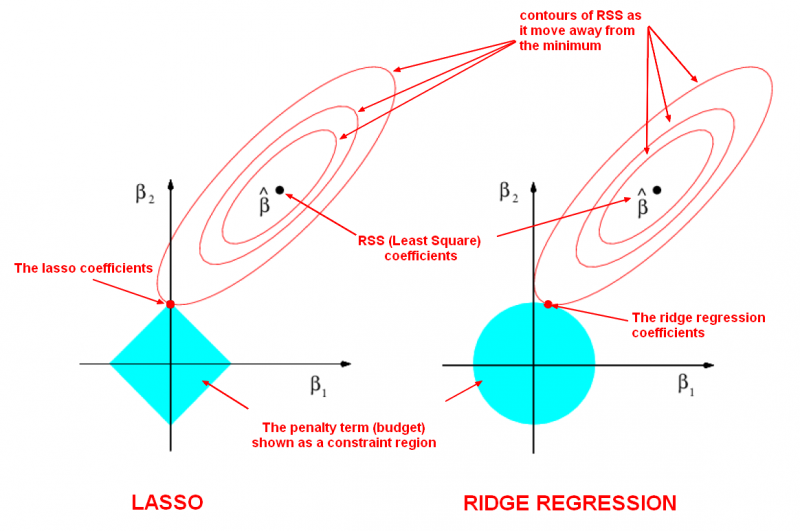
\includegraphics[scale=0.5]{Chap8-ChoixModeleRLM/Figures/lasso_vs_ridge_regression}
\caption[Illustration de la différence entre le LASSO et la régression ridge.]{Illustration de la différence entre le LASSO et la régression ridge. \\{\footnotesize Source : \url{http://gerardnico.com/wiki/data_mining/lasso}}}
\label{fig:lasso}
\end{figure}

\newpage

Tel qu'indiqué plus haut, il faut choisir le paramètre $\lambda$ pour obtenir une estimation avec le LASSO. Celui-ci est généralement choisi pour minimiser l'erreur de prévision, telle qu'estimée par une méthode comme la validation croisée.

Notons que sous certaines hypothèses, on peut montrer que le LASSO identifie correctement les coefficients qui ne valent pas 0 avec une grande probabilité. Toutefois, les estimateurs sont en général biaisés vers 0, et pas nécessairement convergents. En pratique, on utilise donc parfois le LASSO pour faire une sélection de variables, et on estime ensuite les coefficients avec la méthode des moindres carrés sans pénalité.

Enfin, un autre avantage de la régression LASSO est qu'elle permet d'ajuster un modèle dans le cas où le nombre de paramètres à estimer $p'$ est supérieur au nombre d'observations $n$.

\newpage

\section{Le cas des variables catégoriques et interactions}

Dans le cas de modèles de régression contenant des variables catégoriques et des interactions, il faut être un peu plus prudent dans la sélection de modèle.

\subsection{Sélection de modèle avec variables catégoriques}

La sélection se fait comme à l'habitude en présence de variables dichotomiques.

Avec des variables polytomiques, la règle utilisée en sélection de modèle, quel que soit le
critère de sélection, est que les $\beta$ correspondant à une m\^eme variable polytomique soient ou bien tous exclus du modèle, ou bien tous inclus dans le modèle. On peut aussi décider de fusionner certaines catégories de la variable polytomique si c'est suggéré par la forme du modèle sélectionné.

\begin{exemple}
Considérons de nouveau l'exemple \ref{eg:lot}. Si un critère de sélection indique que le meilleur modèle est $Y_i=\beta_0+\beta_{11}x_{11i}+\beta_{13}x_{13i}+\varepsilon_i$, alors on ajoutera $\beta_{12}x_{12i}$ à ce modèle car $\beta_{11}$, $\beta_{12}$ et $\beta_{13}$ sont tous reliés à la variable \og lot \fg et doivent donc ou tous \^etre inclus dans le modèle, ou tous \^etre exclus du modèle, et comme au moins un
de ces $\beta$ semble important, nous les incluons tous. On pourrait aussi décider de fusionner les lots 1 et 2 pour créer une nouvelle variable à trois catégories.
\end{exemple}




\subsection{Sélection de modèle en présence d'interactions}

Si une interaction entre plusieurs variables exogènes est incluse
dans un modèle, on laisse en général les effets plus simples
correspondants dans le modèle. Ceci facilitera l'interprétation des différents coefficients du modèle.

\begin{exemple}
Supposons que le modèle complet est
$$Y=\beta_0+\beta_1x_{1}+\beta_2x_{2}+\beta_3x_{3}+
\beta_{12}x_{1}x_{2}+\beta_{13}x_{1}x_{3}+\beta_{23}x_{2}x_{3}+\varepsilon,$$
mais que les procédures de sélection de variables indiquent que seulement les coefficients $\beta_1$ et $\beta_{23}$
semblent importants.
Nous utiliserions alors le modèle
%$$Y_i=\beta_0+\beta_1x_{1i}+\beta_2x_{2i}+\beta_3x_{3i}+\beta_{23}x_{2i}x_{3i}+\varepsilon_i$$
$$Y=\beta_0+\beta_1x_{1}+\beta_2x_{2}+\beta_3x_{3}+\beta_{23}x_{2}x_{3}+\varepsilon$$
car avec la présence de $\beta_{23}$ dans le modèle, il est
recommandé d'y inclure $\beta_2$ et $\beta_3$.
\end{exemple} 


\chapter{Multicolinéarité}
\label{sec:Multicolinéarité}

\section{Introduction et définition}
Depuis le début du cours, nous avons supposé que la matrice  $\boX$ est une matrice de plein rang, c'est-à-dire qu'il existe une unique inverse à la matrice $\boX'\boX$, et donc qu'il n'existe qu'un seul vecteur $\hbobeta$ qui minimise la somme des carrés résiduels $SC_{\text{res}}$. Toutefois, en pratique certaines colonnes de $\boX$ peuvent être reliées linéairement entre elles. C'est ce qu'on nomme la  multicolinéarité.

%Si certaines colonnes de $X$ sont reliées linéairement entre elles, alors cet inverse n'est plus unique et on ne peut aller plus %loin. Par contre, si certaines colonnes ne sont pas exactement liées de façon linéaire mais sont près de l'être, alors il est %quand même possible de trouver un unique estimateur $\hbobeta$.
La définition mathématique formelle de la multicolinéarité est la suivante.
\begin{defn}\label{def:multi}
Il y a \textbf{multicolinéarité exacte} lorsqu'une variable est la combinaison linéaire d'une ou de plusieurs autres variables, c'est-à-dire  lorsqu'il existe une
 combinaison de constantes $d_1,\ldots,d_p$ (pas toutes \'egales
 \`a z\'ero) telle que
 $$\sum_{j=1}^pd_jX_j=\boz.$$
\end{defn}

\begin{defn}
La \textbf{multicolinéarité} au sens large se produit lorsqu'il existe une
combinaison de constantes $d_1,\ldots,d_p$ (pas toutes \'egales
 \`a z\'ero) telle que
 $$\sum_{j=1}^pd_jX_j\approx \boz.$$
 \end{defn}
Dans le cas de multicolinéarité exacte, la matrice $\boX'\boX$ n'est pas inversible et la régression n'est pas possible.
La multicolinéarité exacte ne représente pas un problème : elle se détecte facilement et il suffit d'enlever la ou les variables en cause pour régler le problème.
La multicolinéarité au sens large est plus fréquente et plus difficile à détecter.

La multicolinéarité au sens large pose plusieurs problèmes :
\begin{enumerate}
  \item Instabilité de $(\boX'\boX)^{-1}$, ce qui entraîne qu'une petite variation en $\boY$ peut se traduire par de très grands changements en $\hbobeta$ et en $\hY$.
  \item On observe des $\hat{\beta}_i$ de signe inattendu ou contre-intuitif.
  \item Les variances des $\hat{\beta}_i$ et des $\hat{Y_i}$ sont très grandes.
  \item Les méthodes de sélection de variables ne concordent pas.
  \item Certains paramètres peuvent se révéler non-significatifs alors que la corrélation des variables correspondantes avec $Y$ est très grande.
\end{enumerate}

Le problème, au fond, est que les variables s'expliquent entre elles. Si on s'imagine l'espace d'une régression à deux variables, c'est comme si les points étaient alignés en «piquets de clôture». Ce phénomène n'est pas facile à détecter dans un espace à haute dimension. Nous présenterons ici quelques outils de détection de la multicolinéarité.

\section{Détection de la multicolinéarité}
\subsection{La matrice de corrélations}
À première vue, on pourrait être tenté de calculer la matrice des corrélations entre les variables exogènes pour détecter la multicolinéarité.

Le coefficient de corrélation échantillonnal entre la variable $x_j$ et la variable $x_k$ est donné par
$$r_{jk}=\dfrac{1}{n-1}\sum_{i=1}^n\frac{(x_{ji}-\overline x_j)(x_{ki}-\overline x_k)}{s_js_k}, \;j\in\{1,\ldots,p\},k\in\{1,\ldots,p\}$$
où $\overline x_j=\sum_{i=1}^n x_{ji}/n$ et $s_j=\sqrt{\sum_{i=1}^n(x_{ji}-\overline x_j)^2/(n-1)}$, et de même pour $\overline x_k$ et $s_k$.

On peut aussi écrire la matrice des coefficients de corrélation échantillonnaux (en excluant la colonne de 1) comme
\begin{eqnarray*}
\boX_c^{*'}\boX_c^{*}=\left(\begin{array}{cccc}
1 & r_{12} &  \cdots & r_{1p} \\
r_{21} & 1 & \cdots & r_{2p} \\
\vdots & \vdots & \ddots  & \vdots \\
r_{p1} & r_{p2} & \cdots  & 1
\end{array}
\right)
\end{eqnarray*}
où $$\boX_c^*=\left(\frac{\bo{x}_1-\overline{\bo{x}}_1}{\sqrt{\sum_i (x_{1i}-\overline x_1)^2} }\;\;\frac{\bo{x}_2-\overline{\bo{x}}_2}{\sqrt{\sum_i (x_{2i}-\overline x_2)^2}} \ldots \frac{\bo{x}_p-\overline{\bo{x}}_p}{\sqrt{\sum_i (x_{pi}-\overline x_p)^2}}  \right)\quad \text{ et } \quad \overline{\bo{x}}_j=(\overline x_j,\ldots,\overline x_j)'.$$



Si deux variables exogènes sont linéairement reliées, leur coefficient de corrélation devrait
être élevé. Cependant deux problèmes majeurs empêchent les coefficients de corrélation
d'être des bons outils de diagnostic:
\begin{itemize}
\item[(i)] il est difficile de dire ce qu'est une grande valeur de la corrélation
\item[(ii)] la multicolinéarité est souvent induite par une dépendance linéaire entre plus de deux variables.
\end{itemize}
Pour voir que le point (ii) constitue un
problème, il est possible de créer des exemples où $p$ variables sont parfaitement linéairement
dépendantes, mais où les coefficients de corrélation de toutes les paires de variables sont
inférieurs à $1/(p-1)$. Ainsi, même si la corrélation entre deux variables est indésirable, cela
ne représente qu'un cas particulier de la multicolinéarité.

\subsection{Le facteur d'inflation de la variance (VIF)}
\label{sec:vif}
Une approche plus sensible consiste à évaluer le degré de dépendance linéaire de chaque
variable exogène sur les autres variables exogènes. Ainsi pour la $j^e$ variable exogène,
on peut mesurer ce niveau de dépendance en effectuant une régression linéaire avec la $j^e$
variable exogène comme variable réponse et les $p-1$ variables exogènes restantes comme variables explicatives. Le coefficient de détermination de cette régression, noté $R^2_j$, mesurera la proportion de la variabilité de la $j^e$ variable exogène qui est expliquée de fa\c{c}on linéaire par les autres variables exogènes. Si $R_j^2$ est grand, on a vraisemblablement un problème.

Cette idée se matérialise dans le facteur d'inflation de la variance (en anglais, VIF pour Variance Inflation Factor). Celui-ci est défini de la façon suivante :
\begin{eqnarray}
  \mbox{VIF}_j &=& \frac{1}{1-R_j^2}
\end{eqnarray}
Si $R_j^2\rightarrow 1$, alors $VIF_j\rightarrow \infty$. Ainsi, une grande valeur de $\mbox{VIF}_j$ signifie une valeur proche de 1 de $R_j^2$, et donc une forte dépendance linéaire des variables exogènes.

Le nom \og facteur d'inflation de la variance \fg  $\;$ vient du fait que la variance de $\hat{\beta}_j$ s'exprime en fonction du VIF comme suit :
\begin{eqnarray*}
% \nonumber to remove numbering (before each equation)
  \var[\hat{\beta}_j] &=& \frac{\sigma^2}{(\boX'\boX)_{jj}} \mbox{VIF}_j
\end{eqnarray*}
On voit donc l'effet de cette multicolinéarité sur la variance des estimateurs des coefficients.

 Plusieurs
auteurs suggèrent un VIF > 10 comme point où l'on doit commencer à considérer la présence
de multicolinéarité aux conséquences importantes. Cependant, les VIF à eux seuls ne sont
pas un diagnostic complet. Parmi les points faibles des VIF on dénote
\begin{itemize}
\item [(i)]l'incapacité de détecter des multicolinéarités impliquant la colonne de 1 de la matrice d'incidence
\item [(ii)] l'incapacité de cerner le nombre de quasi dépendances linéaires présentes dans les données
\item [(iii)] le fait qu'on a jamais réussi à cerner une valeur précise pour le VIF où l'on doit vraiment commencer à s'inquiéter (10 est une valeur \textit{ ad hoc}).
\end{itemize}

\begin{remarque}
Une mesure équivalente au facteur d'inflation de la variance est la tolérance définie comme suit :
$$\mbox{TOL}_j=1-R_j^2=1/\mbox{VIF}_j.$$
La tolérance $\mbox{TOL}_j$ est donc la partie de la variabilité dans la j$^{\text{ème}}$ variable exogène qui n'est pas expliquée par les autres variables exogènes. Ainsi, si on définit un cas problématique comme un cas où $\mbox{VIF}>10$, ceci est équivalent à définir les cas problématiques comme ceux ayant une $\mbox{TOL}< 10 \%$, c'est-à-dire ceux pour qui au moins 90 \% de la variabilité est expliquée par les autres variables exogènes.
\end{remarque}

\subsection{L'indice de conditionnement}

\label{sec:FacteurDeConditionnement}
L'approche la plus efficace afin de détecter les causes de multicolinéarité est basée sur les valeurs propres de la matrice des coefficients de corrélation échantillonnaux $\boX_c^{*'}\boX_c^*$, ou sur la matrice des valeurs réduites, mais non centrées $\boX^*$ (qui permet l'inclusion de la colonne de 1), où 

$$\boX^*=\left(\frac{\bo{x}_1}{\sqrt{\sum_i x_{1i}^2} }\;\;\frac{\bo{x}_2}{\sqrt{\sum_i x_{2i}^2}} \ldots \frac{\bo{x}_p}{\sqrt{\sum_i x_{pi}^2}}  \right).$$

En se servant de la décomposition en valeurs propres de $\boX^{*'}\boX^*$, i.e.
$$\boX^{*'}\boX^*=\bo{P}\bo{\Lambda} \bo{P}'$$
avec $\bo{\Lambda}=\text{diag}(\lambda_1,\ldots,\lambda_{p'})$ et $\bo{P}\bo{P}'= \bo{P}'\bo{P}=\bo{I}_p$, on peut alors montrer que
\begin{equation}
\text{tr}(\boX^{*'}\boX^*)=\text{tr}(\bo{P}\bo{\Lambda} \bo{P}')=\mbox{tr}(\bo{P}'\bo{P}\bo{\Lambda})=\mbox{tr}(\bo{\Lambda})=\sum_{j=1}^{p'}\lambda_j=p'.
\label{eq:traceIC}
\end{equation}
En présence de multicolinéarité, le déterminant de $\boX^{*'}\boX^*$, qui est égal à $\prod\limits_{j=1}^{p'}\lambda_j$, aura une valeur proche de 0.



Ainsi, en présence de multicolinéarité l'équation \ref{eq:traceIC} indique que la somme des valeurs propres doit être égale à $p'$, mais que leur produit sera proche de 0. Puisque les valeurs propres sont toutes positives, cela implique qu'en présence de multicolinéarité, il y aura \`a la fois des valeurs propres de grandes et de faibles valeurs. Le nombre de $\lambda_j$ proche de 0 indique le nombre variables en multicolinéarité. Dans cette situation, le rapport de la plus grande valeur propre sur la plus faible sera donc élevé.

Les \textbf{indices de conditionnement} notés $\eta_j$ pour ${j=1,2,\cdots,p'}$ sont définis comme les racines carrées des rapports entre la plus grande valeur propre de la matrice $\boX^{*'}\boX^*$ et chacune de ses autres valeurs propres, c'est-à-dire
$$\eta_j=\sqrt{\frac{\lambda_{max}}{\lambda_j}}.$$

Plusieurs auteurs semblent s'entendre pour dire qu'une valeur de $\eta_j > 30$ indique une multicolinéarité dont il faut se
soucier.

La plus grande valeur de $\eta_j$ est égale à
$$\kappa=\frac{\lambda_{max}}{\lambda_{min}}.$$

$\kappa$ est parfois appelée \textbf{ facteur de conditionnement}.


%Les valeurs propres $\lambda_1, ..., \lambda_{p'}$ de $(\boX^'\boX)^{-1}$ sont réelles et positives. On peut écrire $(\boX'\boX)=\bo{P}\bo{\Lambda} \bo{P}'$ où $\bo{P}$ est la matrice orthogonale des vecteurs propres et $\bo{Lambda}$ est la matrice diagonale des valeurs propres de $(\boX'\boX)$.
%
%Il y a multicolinéarité lorsque $\lambda_{p'}$, la plus petite valeur propre de $\boX'\boX$, est proche de 0. Rappelons que le déterminant de $\mbox{det}(\boX'\boX)= \prod_{i=1}^{p'} \lambda_{i}=0$ lorsque $\lambda_{p'}=0$. Donc, si $\lambda_{p'}\cong 0$, $(\boX^'\boX)^{-1}$ est instable numériquement.
%
%
% à continuer ici. vérifier la définition du facteur de conditionnement.
%

%Le facteur de conditionnement est un indicateur de la multicolinéarité qui utilise les valeurs propres de la matrice $(\boX^{*'}\boX^*)$. On  le définit de la façon suivante:
%\begin{eqnarray}
%% \nonumber to remove numbering (before each equation)
%  \kappa &=& \sqrt{\frac{\lambda_{\text{max}}}{\lambda_{\text{min}}}}.
%\end{eqnarray}
%Bien que ceci n'ait pas de véritable fondement, on considère généralement un $\kappa>30$ comme étant problématique.

Soit $\bo{p}_j$, le vecteur propre correspondant à la valeur propre $\lambda_j$.
%Les éléments de ces vecteurs peuvent nous aider à identifier le nombre de quasi dépendances linéaires dans les données, et quelles variables exogènes font partie de chaque quasi dépendance. En effet,
Étant donné que
$$\var[\hat\beta_{k-1}]=\sigma^2(\bo{X}^{*'}\bo{X}^*)^{-1}_{kk}=\sigma^2\sum_{j=1}^{p'}p_{kj}^2/\lambda_j,$$
la portion de variance de $\hat\beta_{k-1}$ expliquée par la $j^{e}$ dépendance linéaire peut se mesurer comme suit :
$$v_{kj}=\frac{p_{kj}^2/\lambda_j}{\sum\limits_{l=1}^{p'}p_{kl}^2/\lambda_l}.$$

Pour détecter la multicolinéarité on suit donc la procédure suivante:
\begin{enumerate}
\item Calculer les indices de conditionnement $\eta_j$ et vérifier si certains d'entre eux possèdent une valeur supérieure à 30.
\item Pour chaque $\eta_j$ dont la valeur excède 30, calculer les proportions de la variance $v_{1j},v_{2j},\cdots,v_{p'j}$.
\item Les variables exogènes correspondant aux coefficents avec des valeurs de $v_{kj}$ élevées (en général nettement supérieures à 60 \%) sont multicolinéaires.
\end{enumerate}

\section{Les solutions possibles à la multicolinéarité}
\label{sec:solutionsMulticolinearite}

La solution la plus simple est de retirer une ou plusieurs variables exogènes. Typiquement, on retranchera les variables ayant le plus grand VIF, une à la fois. Dans la pratique, ce retrait des variables doit se faire en collaboration étroite avec le client, car dans le choix des variables, c'est d'abord l'interprétation qui compte. Il est parfois possible  de combiner des variables exogènes redondantes, par exemple pour calculer un score à partir de plusieurs variables exogènes.

Quelques autres solutions sont également disponibles.



\subsection{La régression \og ridge \fg}

La régression ridge, présentée à la section \ref{sec:ridge} peut également être utilisée en cas de multicolinéarité, mais donne des estimateurs biaisés. Ce n'est toutefois pas une option très populaire en pratique.


\subsection{La régression basée sur les composantes principales}


On peut également faire une régression sur les composantes principales de la matrice d'incidence. Les facteurs dans une analyse en composantes principales sont donnés par les colonnes de la matrice $\bo{F}$ suivante :
$\bo{F}=\boX^*\bo{P}$,
où $\bo{P}$ est la matrice des vecteurs propres de $\boX^{*'}\boX^*$. Cette matrice est telle que $\bo{P}'\bo{P}=\bo{P}\bo{P}'=\boI$. En utilisant cette propriété matricielle, nous pouvons écrire le modèle de régression multiple comme
\begin{eqnarray*}
\boY & = & \bo{1}+\boX^*\bobeta + \boeps \\
 & = & \bo{1}+\boX^*\bo{P}\bo{P}'\bobeta+ \boeps\\
& = & \bo{1}+\bo{F}\bo{\gamma}+\epsilon,
\end{eqnarray*}
où $\bo{\gamma}=\bo{P}'\bobeta$ ou encore $\bobeta=\bo{P}\bo{\gamma}$. Le théorème de Gauss-Markov implique que $\hbobeta=\bo{P}\hat{\bo{\gamma}}.$
La multicolinéarité n'est plus présente, mais au prix d'un biais dans les estimateurs. Ce biais est présent si on ne retient dans la modélisation que les facteurs associés aux plus grandes valeurs propres de $\boX^{*'}\boX^*$.

Le principal problème de la régression en composantes principales est son interprétation, qui peut être hasardeuse. %On peut se rattraper en calculant $\hbobeta=\bo{P}\hat{\bo{\gamma}},$ cependant dans ce cas $\esp[\hbobeta]\neq\bobeta$. L'estimation est biaisée.

%Enfin, on peut faire une régression en composantes principales. Pour ce faire, on commence par centrer-réduire la matrice X, on obtient $X^*$. On calcule ensuite la matrice des corrélation $X^{*T}X^*$. On trouve les valeurs propres de cette matrice et on effectue la régression avec le modèle suivant:
%\begin{eqnarray}
%% \nonumber to remove numbering (before each equation)
%  Y &=& Z\alpha + \epsilon
%\end{eqnarray}
%où $Z=X^*P^T$ et $\alpha=P\beta$. On ne retient que le nombre de composantes nécessaires.
%
%Le principal problème de la régression en composantes principales est son interprétation, qui peut être hasardeuse. On peut se rattraper en calculant $\hat{\beta}=P\hat{\alpha}$, mais dans ce cas $E[\hat{\beta}]\neq\beta$; l'estimation est biaisée.


\addtocontents{toc}{\protect\pagebreak}

\chapter{Observations aberrantes et influentes}
\label{sec:DonneesInfluentes}

\vspace{-0.1in}
%Tout comme on a sélectionné les variables à inclure dans le modèle de RLM, il peut être nécessaire de sélectionner les observations à inclure dans le modèle.
On doit parfois retirer du modèle une ou plusieurs observations qui ont une influence trop grande sur l'estimation des paramètres. Avant de parler plus en détails de ces données influentes, il faut bien définir deux termes importants.

\begin{defn}\label{def:aber}
Une observation est \textbf{ aberrante} si elle ne cadre pas avec le modèle.
\end{defn}

\vspace{-0.1in}
Ce sera donc une observation qui a un résidu de grande taille. Une donnée aberrante n'est pas problématique en elle-même, mais elle peut indiquer une erreur dans la valeur d'une variable exogène ou de la variable endogène.

\begin{defn}\label{def:infl}
Une donnée \textbf{influente} est une observation qui, \`a elle seule, peut avoir un impact sérieux sur les conclusions d'une analyse de régression.
\end{defn}

\vspace{-0.1 in}
Parmi les exemples \og d'impact sérieux \fg, on peut citer des $\hat{\beta}$ négatifs quand on sait qu'ils devraient \^etre positifs (ou vice-versa) ou encore une variable exogène qui devrait \^etre importante mais qui est considérée non significative. Une ou des observations influentes peut également diminuer le pouvoir prédictif du modèle.

%\newpage
\section{Sources de l'influence}

L'influence d'une observation provient souvent d'une combinaison de
deux sources :
\begin{description}
\item[Source 1:] L'observation a un grand levier, c'est-à-dire qu'elle a une grande capacité \textit{a priori} à influencer les résultats de la régression.
\item[Source 2:] L'observation a une valeur extrême de $Y$ par rapport au modèle.
%Donnée ayant une erreur produisant une valeur extr\^eme de $Y$.
\end{description}
On peut facilement identifier les observations avec ces deux caractéristiques.

\textbf{Levier d'une observation}

Une observation a un grand levier si sa valeur de $\boldx_i$ est loin du centre (centro\"{\i}de) de toutes les observations. La distance entre une observation et le centro\"{\i}de de toutes les autres peut être calculée facilement à partir de la matrice d'incidence $\boX$. Plus précisément, le levier de la $i^e$ observation est le $i^e$ élément diagonal de la matrice chapeau $\boH=\boX(\boX'\boX)^{-1}\boX'$, qui peut s'exprimer comme
$h_{ii}=\boldx_i'(\boX'\boX)^{-1}\boldx_i$.

Qu'est-ce qu'une grande valeur de $h_{ii}$? Il est difficile de
répondre \`a cette question de fa\c{c}on générale. Cependant nous
savons que tr$(\boH)=\sum_{i=1}^n h_{ii}=p'$, o\`u $p'$ est le nombre
de paramètres dans le modèle. Donc un $h_{ii}$ moyen prend une valeur de $p'/n$
et un $h_{ii}$ qui se démarque nettement de cette valeur
signifie une donnée \`a grand levier. \citet{Bel_Kuh_Wel:80} suggèrent de retenir les valeurs de $h_{ii}>2p'/n$.

\textbf{Observation extrême}

Une observation est extrême (ou aberrante) par rapport au modèle si son résidu est grand. On regardera plus précisément le résidu studentisé. On rappelle que celui-ci est donné par

$$T_i={\hat\varepsilon_i\over \hat\sigma_{-i}\sqrt{1-h_{ii}}} \sim\mathcal{T}_{n-p-2},$$
o\`u $$\hat\sigma_{-i}=\sqrt{{(n-p)\hat\sigma^2-\hat\varepsilon_i^2/(1-h_{ii})\over n-p-1}}.$$

Comme on peut le voir, ce résidu est une fonction croissante à la fois en
$h_{ii}$ et en $\hat\varepsilon_i$.

\citet{Bel_Kuh_Wel:80} prônent de prendre les valeurs de $|T_i|>t_{n-p',(1-\alpha^*/2)}$, où $\alpha^*=\alpha/n$ (le seuil corrigé de Bonferroni) comme un bon indicateur d'une valeur aberrante. D'autres statisticiens suggèrent de retenir les valeurs de $|T_i|>2$.

\begin{remarque}
Avoir un grand levier et être une observation extrême sont des indices qu'une observation pourrait avoir une influence démesurée sur les résultats de la régression. Pour tester si cela est effectivement le cas, on doit mesurer directement l'influence de l'observation sur la régression. Il est important de comprendre qu'une donnée avec un grand levier peut ne pas être influente. Il en est de même pour une observation extrême.
\end{remarque}


%Un grand levier n'implique pas nécessairement une influence. Tout diagnostic d'influence doit \^etre basé sur une combinaison de $h_{ii}$ et $R_{i}$.

\section{Mesures d'influence}

Pour mesurer si une donnée est influente ou non, on évalue son impact sur la prévision $\hY$ et sur l'estimation de $\bobeta$. Les différentes statistiques utilisées sont présentées ici.

\subsection{Influence sur la prévision}
La statistique suivante mesure l'influence de la $i^e$ donnée
dans la prévision $\hat{Y}_i$ de $Y_i$ (\textit{Difference in Fit}) :
$$DFFIT_i={\hat{Y}_i-\hat{Y}_{i,-i}\over
\hat\sigma_{-i}\sqrt{h_{ii}}}=T_i\sqrt{h_{ii}\over1-h_{ii}},$$ o\`u
$\hat{Y}_{i,-i}$ désigne la valeur de la prévision de $Y_i$ basée
sur un jeu de données qui ne contient pas la $i^e$ donnée,
c'est-à-dire $\hat{Y}_{i,-i}=\boldx_i'\hat{\bobeta}_{-i}$.

Il faut se rappeler ici que $\var[\hat Y_i]=\sigma^2h_{ii}$. Les différences au numérateur de $DFFIT_i$ sont donc standardisées de sorte qu'elles s'expriment en multiples de l'écart-type de la prévision.

Nous analysons les $DFFIT_i$ de la m\^eme fa\c{c}on que nous nous penchons sur les $T_i$, c'est-à-dire que des grandes valeurs de $|DFFIT_i|$ constituent un signe que la $i^e$ donnée possède une grande influence sur la valeur de la prévision. \citet{Bel_Kuh_Wel:80} indiquent qu'il faut retenir les valeurs de $|DFFIT_i|>2\sqrt{p/n}$ alors que d'autres statisticiens proposent simplement de retenir les valeurs de $|DFFIT_i|>2$.

\subsection{Influence sur les estimations des paramètres}
La statistique suivante mesure l'influence de la $i^e$
observation sur la valeur de l'estimateur de $\beta_j$ (\textit{ Difference in Beta}):
$$DFBETA_{ji}={\hat{\beta}_j-\hat{\beta}_{j,-i}\over
\hat\sigma_{-i}\sqrt{(\boX'\boX)^{-1}_{jj}}}.$$
Il faut se souvenir ici que $\var[\hat\beta_j]=\sigma^2(\boX'\boX)^{-1}_{jj}$. Les différences au numérateur de la statistique sont  à nouveau standardisées.
Encore une fois, les grandes valeurs de $DFBETA_{ji}$ indiquent que la $i^e$ donnée possède une grande influence sur l'estimation de $\beta_j$. \citet{Bel_Kuh_Wel:80} proposent de considérer les valeurs de $|DFBETA_{ji}|>2/\sqrt{n}$ alors que d'autres statisticiens suggèrent simplement de retenir les valeurs de $|DFBETA_{ji}|>2$. \\

Le signe de $DFBETA_{ji}$ est un bon indicateur. En effet, si un certain $\hat\beta_j$ est négatif alors qu'on se serait attendu à une valeur positive, alors un $DFBETA_{ji}$ très négatif indique que le \og coupable \fg pourrait être l'observation $i$.

Comme nous obtenons $p$ valeurs de $DFBETA$
pour chaque observation, cette mesure devient peu pratique lorsque
nous sommes en présence d'un jeu de données ayant plusieurs
variables exogènes. Pour simplifier la recherche de valeurs influentes, Dennis Cook a proposé la statistique suivante, appelée distance
de Cook, qui permet de combiner les $DFBETA$ d'une m\^eme observation:
\begin{eqnarray*}
\text{distance de Cook}_i\;=\;C_i & = & {(\hat{\bobeta}-\hat{\bobeta}_{-i})'(\boX'\boX)(\hat{\bobeta}-\hat{\bobeta}_{-i})
\over p' \hat\sigma^2} \\
& = & \frac{(\hat Y_i-\bo{x}_i'\hat{\bobeta}_{-i})^2}{p'\hat\sigma^2} \\
& = & \frac{\hat\varepsilon_i^2}{(1-h_{ii})^2}\frac{h_{ii}}{\hat\sigma^2 p'} \\
% & = & \frac{\hat\varepsilon_{i,-i}^2}{p}\frac{h_{ii}}{1-h_{ii}}
\end{eqnarray*}
 Une grande valeur de $C_i$ indique une observation
ayant une influence prépondérante sur les $\beta$. \citet{Fox:91} suggère de porter notre attention sur les valeurs de $C_i>\frac{4}{n-p}$. Il s'agit par la suite
d'examiner les $DFBETA$ pour cette observation pour savoir quel(s)
$\hat\beta$ est (sont) affecté(s).


\subsection{Influence sur la performance des estimateurs}
Une donnée peut aussi avoir un impact néfaste sur la variance des estimateurs. Soit $||Var(\hat{\bobeta})|| = (\sigma^2)^p||(\boX'\boX)^{-1}||$, le déterminant de la matrice de variance de $\hat{\bobeta}$, parfois appelé variance généralisée. L'influence de la $i^e$ donnée sur la variance de $\hat{\bobeta}$ peut \^etre calculée comme suit:

\begin{eqnarray*}COVRATIO_i&=&{||(\boX_{-i}'\boX_{-i})^{-1}\hat\sigma_{-i}^2||
\over||(\boX'\boX)^{-1}\hat\sigma^2||}\\
&=&\left({\hat\sigma_{-i}^{2}\over
\hat\sigma^{2}}\right)^p\left({h_{ii}\over1-h_{ii}}\right).\end{eqnarray*}
Comme la seconde ligne l'illustre, une donnée possédant beaucoup de levier
donnera en général un $COVRATIO>1$, et une donnée aberrante un $COVRATIO<1$.

\citet{Bel_Kuh_Wel:80} proposent de porter notre attention sur les valeurs telles que
$|COVRATIO-1|~>~3p/n$, c'est-à-dire sur les observations telles que\\ $COVRATIO~<~1~-~3p/n$ ou $COVRATIO>1+3p/n$.



\section{Que faire avec les données influentes?}
Si une donnée est influente, il faut prendre tous les moyens
possibles pour essayer de comprendre comment cette donnée a été
obtenue et s'assurer qu'il n'y a pas d'erreur qui aurait pu
survenir lors de la mesure, collecte ou saisie des données.

Si l'influence provient d'un grand
levier, alors il serait souhaitable d'aller chercher d'autres
données afin de combler le vide entre le centro\"{\i}de des
données et la donnée influente.

En général, on doit s'abstenir d'éliminer les données
influentes d'un jeu de données. Quelques exceptions:
\begin{itemize}
\item Erreur de mesure ou  de  saisie (corriger la donnée
est préférable \`a son élimination). \item Valeurs
mesurées scientifiquement peu plausibles. \item Donnée très
peu représentative du reste des données et de la population en
général. \end{itemize}

Il est \`a noter que souvent, une transformation de variable peut
grandement réduire l'influence de certaines données. 

\chapter{Techniques plus avancées}
\label{sec:TechniquesAvancees}

On présente ici quelques techniques de régression plus avancées. Elles peuvent entre autres être utilisées si les postulats de la RLM ne sont pas vérifiés.


\section{Régression polynomiale}
\label{sec:regpoly}

L'idée derrière la régression linéaire est que le modèle
linéaire est une bonne approximation de la \og vraie \fg relation
entre la variable endogène et les variables exogènes
$$Y=f(x_1,x_2,\ldots,x_k)+\varepsilon.$$
Dans plusieurs cas, le modèle de régression linéaire sera
une approximation suffisamment bonne de $f(x_1,\ldots,x_k)$. Par
contre dans certaines situations, il arrive que l'approximation
linéaire ne soit pas assez proche de $f(x_1,\ldots,x_k)$ pour
donner un modèle approprié. Dans ces cas, nous pouvons
utiliser le principe disant que la plupart des fonctions peuvent
\^etre approchées aussi bien que l'on veut par une expansion
polynomiale. Plus il y a de la \og courbure \fg dans
$f(x_1,\ldots,x_k)$, plus le polyn\^ome utilisé pour
approcher $f(x_1,\ldots,x_k)$ doit \^etre de degré élevé
pour que l'approximation soit suffisamment précise.

En régression, ceci se traduit par le résultat suivant:
\begin{eqnarray*}
Y_i&=&f(x_{1i},\ldots,x_{ki})+\varepsilon_i\\
&\approx&\beta_0+\beta_1x_{1i}+\cdots+\beta_kx_{ki}\\
&\ &\ \ \ +\beta_{11}x_{1i}^2+\cdots+\beta_{kk}x_{ki}^2+
\beta_{12}x_{1i}x_{2i}+\cdots+\beta_{k-1,k}x_{k-1,i}x_{ki}\\
&\ & \ \ \ +\beta_{111}x_{1i}^3+\cdots+ \beta_{kk\cdots
k}x_{ki}^d+\cdots+\varepsilon_i.
\end{eqnarray*}
En général, il est rarement nécessaire de dépasser un modèle du second degré:
\begin{eqnarray*}
Y_i&=&\beta_0+\beta_1x_{1i}+\cdots+\beta_kx_{ki}\\
&\ &\ \ \ +\beta_{11}x_{1i}^2+\cdots+\beta_{kk}x_{ki}^2+
\beta_{12}x_{1i}x_{2i}+\cdots+\beta_{k-1,k}x_{k-1,i}x_{ki}.
\end{eqnarray*}

Il est possible que l'on rencontre des problèmes numériques ou
de multicolinéarité quand on utilise des modèles polynomiaux. Si l'objectif est de trouver un modèle faisant de bonnes prédictions, ce n'est pas vraiment un problème. Si on veut vraiment interpréter les valeurs des coefficients de chaque terme, alors on peut travailler avec les variables exogènes standardisées, c'est-à-dire de
remplacer $x_{ji}$ par
$$x_{ji}^*=\frac{(x_{ji}-\bar{x}_j)}{s_j}$$

$ \mbox{ o\`u } \bar{x_j}=\sum_ix_{ji}/n \mbox{ et } s_j^2=\sum_i(x_{ji}-\bar{x}_j)^2/(n-1).$

\subsubsection*{Sélection de modèle}

Comme c'était le cas avec les interactions, si un terme de
degré $d$ est inclus dans le modèle, alors en général on
inclut les termes de degré inférieur \`a $d$.% composés des termes présents dans le terme de degré $d$ en question.


%\noindent\textbf{Note:} Il est préférable d'utiliser une transformation de $Y$ et/ou de certains des $x$ si cette transformation donne d'aussi bons résultats qu'un modèle polynomial avec moins de paramètres. Par exemple, $$\ln Y_i=\beta_0+\beta_1x_{1i}+\varepsilon_i$$ ou $$Y_i=\beta_0+\beta_1e^{x_{1i}}+\varepsilon_i$$ peut \^etre préférable \`a $$Y_i=\beta_0+\beta_1x_{1i}+\beta_2x_{1i}^2+\beta_3x_{3i}^3+\varepsilon_i.$$ Un examen des résidus et de la valeur des critères de sélection de modèle aident souvent \`a déterminer quel modèle est le plus approprié pour vos données.


\subsubsection*{Test de comparaison de modèle pour justifier un degré supérieur}

% Tout comme c'était le cas avec les termes d'interaction, des termes de degré supérieur peuvent \^etre ajoutés \`a un modèle afin d'en vérifier l'ajustement.

\begin{exemple}
Soit le modèle
$Y=\beta_0+\beta_1x_{1}+\beta_2x_{2}+\varepsilon.$

Ce modèle est-il aussi valide que celui contenant des termes de degré 2?
$$Y=\beta_0+\beta_1x_{1}+\beta_2x_{2}+\beta_{11}x_{1}^2
+\beta_{22}x_{2}^2+ \beta_{12}x_{1}x_{2}+\varepsilon.$$

Nous pouvons utiliser un test $F$ de comparaison de modèles pour les hypothèses\\
$H_0:\ \beta_{11}=\beta_{22}=\beta_{12}=0$ contre \\
$H_1:$ au moins un de ces $\beta$ diffère de 0. \\

Si nous ne rejetons pas $H_0$, alors le modèle de premier degré est adéquat. Si nous rejetons $H_0$, alors le modèle de premier degré n'est pas adéquat.\\

On aurait pu vérifier l'ajout d'un seul terme à la fois, car il est fort possible qu'une relation quadratique soit souhaitable en $x_1$ mais pas en $x_2$.
\end{exemple}


\newpage

\section{Régression non linéaire}


Si l'espérance de $Y$ (ou de $g(Y)$) n'est pas une fonction linéaire des variables indépendantes, mais qu'on a une idée de la vraie relation entre $Y$ et les variables indépendantes, on peut néanmoins estimer les paramètres de cette relation non linéaire avec la méthode des moindres carrés. Il n'y a pas de solution analytique dans ce cas, mais des  méthodes numériques peuvent minimiser la somme des carrés des erreurs.

\begin{exemple}
Dans une expérience sur des rats, on trempe  des portions du ventricule auriculaire gauche dans une solution de chlorure de calcium, puis on stimule électriquement le tissu et on mesure la longueur du rétrécissement de la bandelette de tissu.
On s'intéresse à la relation entre
\begin{itemize}
\item[] x :  la concentration de chlorure de calcium (en mM)
\item[] Y : le changement de longueur de la bandelette en réaction au choc (en mm)
\end{itemize}
La figure \ref{fig:rat1} illustre les données. Il est clair qu'un modèle linéaire n'est pas approprié.

Il se trouve toutefois qu'on a déjà une idée du modèle approprié pour les données:
$$ Y_i =  \alpha + \beta e^{-x_i / \theta} + \varepsilon_i $$
La régression non linéaire permet d'estimer les coefficients par la méthode des moindres carrés. On trouve $\hat\theta = 0,6082$, $\hat\alpha = 28,9633$ et $\hat\beta = -34,2274$. La fonction de régression correspondante est également illustrée à la figure \ref{fig:rat1}.

\begin{figure}[h!]
\centering
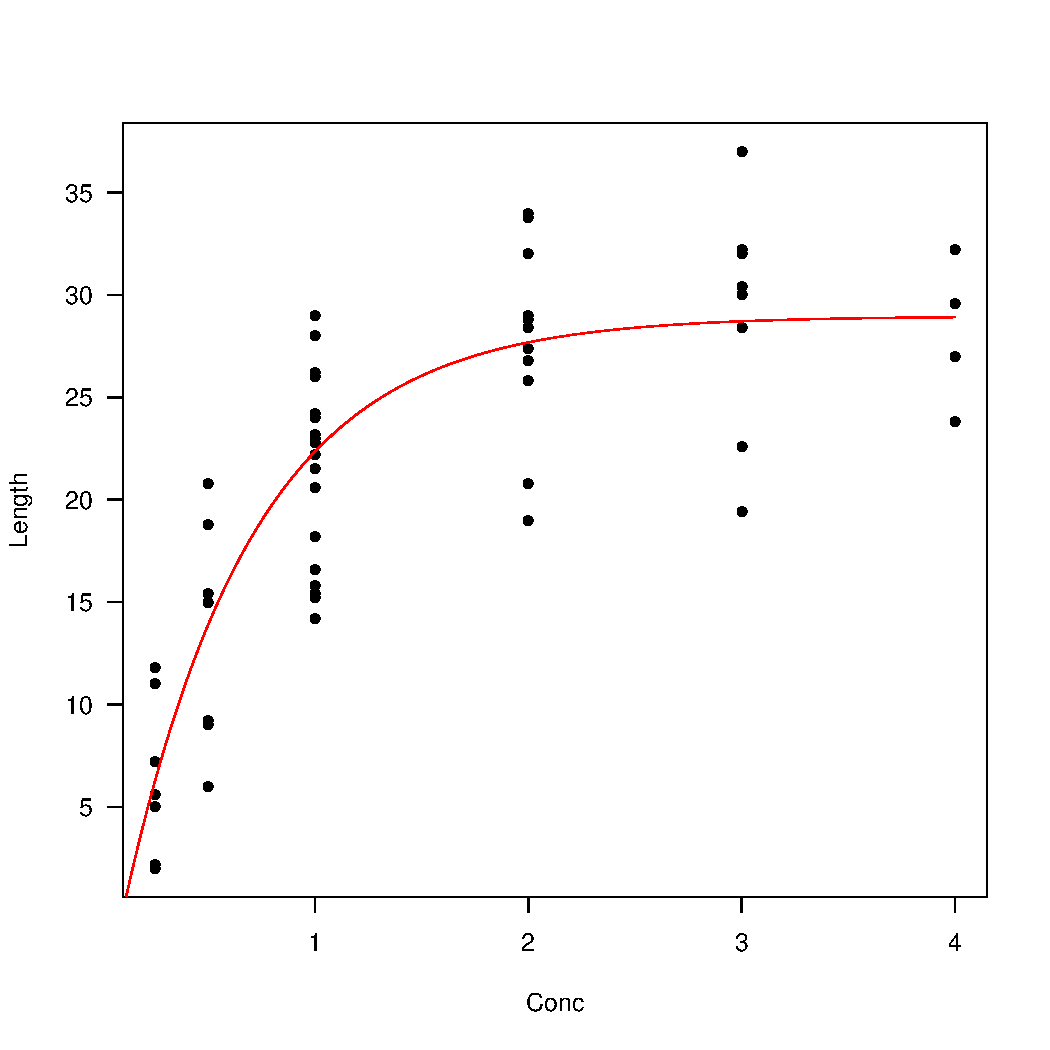
\includegraphics[scale=0.5]{Chap11-TechniquesAvancees/Figures/Nonlinear2}
\caption{Données d'une expérience sur des rats de laboratoire avec la fonction de régression estimée}
\label{fig:rat1}
\end{figure}
\end{exemple}


\newpage
\section{Régression pondérée}


La méthode des moindres carrés pondérés consiste \`a attribuer un poids différent  à chaque observation, et donc à trouver $\hat{\bobeta}$ tel que
$$\sum_{i=1}^nw_i(Y_i-\hat{Y}_i)^2$$
est minimale, o\`u $w_i$ est le poids associé à l'observation $i$.

Une application fréquente de la régression pondérée est lorsque l'hypothèse d'homo\-scédasticité n'est pas respectée, c'est-à-dire si le modèle est plutôt caractérisé par \\$\boeps\sim \mathcal{N}_n(\boz,\mbox{diag}(\sigma_1^2,\ldots,\sigma_n^2))$, o\`u $\sigma_i^2\neq\sigma^2$ pour tout $i$.


Le choix des poids $w_i$ n'est pas toujours facile à faire. Si chaque observation est en réalité la moyenne de $n_i$ valeurs, on peut utiliser un poids égal $w_i=n_i$. Si la variance des erreurs est liée à une variable explicative, on peut faire un graphe des paires $(x_i,\, t_i)$, et voir
comment la variance des résidus studentisés évolue en
fonction de $x_i$. Si le graphe est en forme d'entonnoir ouvert
vers la droite, alors on pourra prendre $w_i=1/x_i$,
$w_i=1/\sqrt{x_i}$, $w_i=1/x_i^{2}$, etc. Si l'entonnoir ouvre vers
la gauche, alors on peut prendre $w_i=x_i$, $w_i=\sqrt{x_i}$,
$w_i=x_i^{2}$, etc. Il est toutefois recommandé d'essayer d'abord de régler le problème à l'aide d'une transformation de variable.

En régression linéaire multiple, il y a plusieurs variables explicatives, il faut donc trouver une stratégie plus globale en cas d'hétéroscédasticité. 
L'idéal serait d'identifier des poids de la forme $w_i\propto1/\sigma^2_i \;$, où $\sigma_i^2$ est la variance de l'erreur pour l'observation $i$. On peut démontrer que dans ce cas,
$$\hat{\bobeta}=(\boX'\boV^{-1}\boX)^{-1}\boX'\boV^{-1}\boY,$$
o\`u $\boV=\mbox{diag}(\sigma_1^2,\ldots,\sigma_n^2)$. La variance de
$\hat{\bobeta}$ est alors
\begin{eqnarray*}
\var(\hat{\bobeta})&=&(\boX'\boV^{-1}\boX)^{-1}\boX'\boV^{-1}\;\boV\;\boV^{-1}\boX(\boX'\boV^{-1}\boX)^{-1}\\
&=&(\boX'\boV^{-1}\boX)^{-1}.
\end{eqnarray*}
On pourrait donc tester $H_0:\beta_j=c$ en utilisant la statistique
$$t={\hat{\beta}_j-c\over
\sqrt{(\boX'\boV^{-1}\boX)^{-1}_{jj}}}.$$ 

Or, établir des estimations des $\sigma_i$ n'est pas si évident.  Voici quelques pistes de solutions (il faut d'abord ajuster une régression du modèle complet et s'assurer que la linéarité est respectée):

\begin{itemize}
\item Si le graphique des $\hat\varepsilon_i$ en fonction des $\hat Y_i$ est en entonnoir, on ajuste une régression des $|\hat\varepsilon_i|$ sur les $\hat Y_i$. Les valeurs prédites de ce nouvel ajustement sont une estimation de $\sigma_i$. (Et les poids seront $w_i=1/\hat\sigma_i^2$).

\item Si le graphique des $\hat\varepsilon_i^2$ en fonction des $\hat Y_i$ montre une tendance à la hausse, on ajuste une régression des $\hat\varepsilon_i^2$ sur les $\hat Y_i$. Les valeurs prédites de ce nouvel ajustement sont une estimation de $\sigma_i^2$. (Et les poids seront $w_i=1/\hat\sigma_i^2$).
% Source: https://onlinecourses.science.psu.edu/stat501/node/352
\end{itemize}
%Parfois on utilise $\boV=\boV^*\sigma^2$ et on estime $\sigma^2$ par $$s^2={\sum_{i=1}^nw_i(Y_i-\hat{Y}_i)^2\over n-p'}.$$

% Une table d'analyse de variance peut aussi \^etre construite en utilisant la décomposition
% $$ {\underbrace{\boY'\boV^{-1}\boY}\atop SC_{tot:W}}={\underbrace{\hat{\bobeta}\boX'\boV^{-1}\boY} \atop SC_{reg:W}}+{\underbrace{(\boY-\boX\hat{\bobeta})'\boV^{-1}(\boY-\boX\hat{\bobeta})} \atop SC_{res:W}}.$$ 

Quelques remarques sur la régression pondérée:
\begin{itemize}
\item En général, les estimations des $\hat\beta_j$ ne seront pas dramatiquement changées par la régression pondérée.
\item Les degrés de liberté ne sont pas affectés par l'insertion de poids. %calculés de la m\^eme fa\c{c}on qu'en régression linéaire ordinaire.
\item Les intervalles de confiance et les tests d'hypothèses sont affectés par les poids.
% Source: https://onlinecourses.science.psu.edu/stat501/node/352
\end{itemize}

\newpage

\section{Modélisation de la dépendance}

Lorsque l'hypothèse d'indépendance des observations n'est pas vérifiée, on peut modéliser directement la dépendance en ajoutant des paramètres à la matrice de covariance des erreurs. Alors que la régression pondérée permet des valeurs différentes sur la diagonale de la matrice de covariance des erreurs, on modélise la dépendance en remplaçant les zéros hors diagonale par des paramètres à estimer. Selon la dépendance que l'on souhaite modéliser, on paramétrisera la matrice de covariance différemment.


Une forme particulière de dépendance est l'autocorrélation, qui arrive lorsque le résidu d'une observation est relié à celui de l'observation précédente, par exemple dans une série temporelle. Un modèle dit autorégressif peut alors être utilisé pour ajuster un modèle de régression.

Mathématiquement, on écrit
\begin{equation}\label{ar1}
\varepsilon_i=\rho\varepsilon_{i-1}+u_i, \end{equation} o\`u
$u_1,\ldots,u_n$ sont i.i.d. $\mathcal{N}(0,\sigma_u^2)$. Le paramètre
$\rho$ dans (\ref{ar1}) est nommé paramètre
d'au\-to\-cor\-ré\-la\-tion, et sa valeur doit \^etre dans
l'intervalle (-1,1).

\`A partir de (\ref{ar1}), nous pouvons
calculer directement que
\begin{eqnarray*}
\varepsilon_i&=&\sum_{j=0}^\infty\rho^ju_{i-j}\\
\esp[\varepsilon_i]&=&\sum_{j=0}^\infty\rho^j\esp[u_{i-j}]=0\\
\var[\varepsilon_i]&=&\sigma_u^2\sum_{j=0}^\infty\rho^{2j}={\sigma_u^2\over1-\rho^2}\\
\cov(\varepsilon_i,\varepsilon_{i+j})&=&\rho^{|j|}{\sigma_u^2\over1-\rho^2}.
\end{eqnarray*}
Comme on peut le voir, une autocorrélation positive entre
$\varepsilon_i$ et $\varepsilon_{i+1}$ est obtenue lorsque $\rho>0$,
tandis que $\rho<0$ donne une autocorrélation négative. Il n'y a
pas d'autocorrélation lorsque $\rho=0$.



%\section{Régression non-paramétrique}

\section{Autres}

Il existe plusieurs autres modèles de régression plus complexes, notamment la régression linéaire mixte, la régression linéaire locale, la régression non-paramétrique, les arbres de régression, etc. 
\appendix

\chapter{Rappels d'algèbre linéaire}

\section{Opérations sur les matrices}

\subsection{Définitions}

\begin{defn}
Une \textbf{matrice} réelle $m\times n$ est un tableau ordonné de nombres réels arrangés en $m$ lignes et $n$ colonnes. On appelle ce tableau matrice de dimension $m \times n$. \\
Notation
$$
A=\left[ \begin{array}{ccccc}
a_{11} & \cdots & a_{1j} & \cdots & a_{1n} \\
\vdots &         & \vdots &           & \vdots \\
a_{i1} &  \cdots       &  a_{ij} & \cdots & a_{in} \\
\vdots &         & \vdots &           & \vdots \\
a_{m1} &  \cdots & a_{mj}& \cdots & a_{mn}
\end{array}
\right]
$$
\end{defn}

\begin{defn}
La \textbf{somme matricielle} $C=A+B$ de deux matrices $A$ ($m\times n$) et $B$ ($m\times n$) est la matrice $C$ (de même dimension que $A$ et $B$) dont les éléments sont
$$c_{ij}=a_{ij}+b_{ij}\qquad\;\;i=1,\ldots,m; j=1,\ldots,n.$$
\end{defn}

\begin{defn}
Soit $A$ une matrice de dimension $m\times n$ quelconque, alors la \textbf{matrice transposée} de $A$, notée $A'$ de dimension $n\times m$ comprend les éléments $\alpha_{ji}=a_{ij},\;\;i=1,\ldots,m; j=1,\ldots,n.$
\end{defn}

\begin{defn}
Le produit du scalaire $k, k\in\R$, par la matrice $A$ de dimension $m\times n$ est la matrice $C$ de dimension $m\times n$, $C=kA$, dont les éléments sont
$$c_{ij}=ka_{ij}\;\;i=1,\ldots,m; j=1,\ldots,n.$$
\end{defn}

\begin{defn}
Soient $A$ et $B$ deux matrices de dimensions respectives $m\times r$ et $r\times n$. Le \textbf{produit matriciel} $C=AB$ correspond à la matrice $C$ de dimension $m\times n$ dont les éléments s'obtiennent comme
$$c_{ij}=\sum_{k=1}^r a_{ik}b_{kj}\;\;i=1,\ldots,m; j=1,\ldots,n.$$
Il est à noter que le produit matriciel n'est défini que si le nombre de colonnes de $A$ est égal au nombre de lignes de $B$. L'élément $c_{ij}$ correspond au produit scalaire euclidien du i$^\text{ème}$ vecteur ligne de $A$ par le j$^\text{ème}$ vecteur colonne de $B$.
\end{defn}



\subsection{Propriétés du calcul matriciel}
\label{sec:prop_calc_mat}

En supposant des matrices compatibles pour les opérations en question, on a que

\begin{enumerate}
\item Commutativité de la somme : $A + B  =  B + A$
\item Associativité de la somme : $(A+B)+C  =  A+ (B+C)$
\item Associativité du produit:  $(AB)C=A(BC)$
\item Divers types de distributivité :\\
$A(B+C)=AB+AC$ \\
$(A+B)C=AC+BC$ \\
$k(A+B)=kA+kB$ \\
$(k_1+k_2)A=k_1A+k_2A$
\item Divers types d'associativité : \\
$k_1(k_2C)=k_1k_2C$  \\
$k(AB)=(kA)B=A(kB)$
\end{enumerate}


\subsection{Propriétés de la transposition}
\label{sec:prop_transp}
\begin{enumerate}
\item
$(A+B)'=A'+B'$
\item
$(kA)'=kA'$
\item
$(AB)'=B'A'$
\item
$(A')'=A$
\end{enumerate}

\section{Espérance et variance de combinaisons linéaires de variables aléatoires}

 Soit $\boY=(Y_1\ Y_2\ \cdots\ Y_n)'$, un vecteur de
$n$ variables al\'eatoires et $\bo{A}$ et $\bo{B}$, des matrices de constantes. L'espérance et la variance de $\boY$ s'écrivent sous forme matricielle comme
\begin{eqnarray*}
\esp[\boY]&\equiv&\left(\begin{array}{c} \esp[Y_1]\\ \esp[Y_2]\\ \vdots \\ \esp[Y_n]\end{array}\right)\
\ \var[\boY]\equiv\left(\begin{array}{cccc}
\var[Y_1] & \cov(Y_1,Y_2) & \cdots & \cov(Y_1,Y_n) \\
\cov(Y_2,Y_1) & \var[Y_2] & \cdots & \cov(Y_2,Y_n) \\
\vdots & \vdots & \ddots & \vdots \\
\cov(Y_n,Y_1) & \cov(Y_n,Y_2) & \cdots & \var[Y_n]\end{array}\right)\\
\end{eqnarray*}
Les propriétés de l'espérance et de la variance sous forme matricielle sont
\begin{eqnarray*}
\esp[\bo{A}\boY+\bo{B}]&=&\bo{A}\esp[\boY]+\bo{B} \\
\var[\bo{A}\boY] &= & \bo{A}\var[\boY]\bo{A}' \\
\var[\bo{A}\boY+\bo{B}] & = & \bo{A}\var[\boY]\bo{A}'.
\end{eqnarray*} 

\chapter{La loi normale multivariée}
\label{LaLoiNormaleMultivariée}

Rappelons d'abord quelques notions sur la loi normale univariée.

Dans le cas d'une variable aléatoire $Z$ distribuée selon une loi normale centrée réduite $Z\sim\N(0,1)$, la densité de $Z$ s'écrit comme
\begin{eqnarray*}
 f_Z(z) = \frac{1}{\sqrt{2\pi}} \exp(-z^2/2)
\end{eqnarray*}
Une variable $X$ de distribution normale avec moyenne $\mu$ et variance $\sigma^2$ s'obtient comme $X=\sigma Z+\mu$. On dit dans ce cas que $X \sim \N (\mu,\sigma^2)$. La densité de cette variable $X$ s'exprime comme
\begin{eqnarray*}
	f_X(x) =  \frac{1}{\sqrt{2\pi} \sigma} \exp\left\{-\frac{1}{2} \left(\frac{x- \mu}{\sigma}\right)^2\right\}.
\end{eqnarray*}

On considère maintenant la généralisation pour $p\geq 1$.  En posant $\bo{Z}=[Z_1, Z_2, ..., Z_p]'$ un vecteur de variables aléatoires indépendantes et identiquement distribuées suivant chacune une loi  $\N(0,1)$, on a que la densité conjointe des $Z_i$ peut  s'écrire comme
\begin{eqnarray}
 f(Z_1, ..., Z_p) &=& \prod_{i=1}^p f(z_i)\nonumber\\
  &=& \left(\frac{1}{\sqrt{2\pi}}\right)^p \exp\left(-\sum_{i=1}^p z_i^2/2\right)\nonumber\\
 &=& \left(\frac{1}{\sqrt{2\pi}}\right)^p \exp\left(-\frac{1}{2} \bo{Z}'\bo{Z}\right)
\end{eqnarray}

Cette densité conjointe est une loi normale multivariée de dimension $p$, dont le vecteur des espérances est \textbf{0} (un vecteur $p\times 1$ de zéros) et dont la matrice de variances-covariances est $\I_p$ (la matrice identité de dimension $p \times p$). On peut donc écrire
\begin{eqnarray*}
 \left[
\begin{MAT}(r)[2pt,0pt,3cm]{c}
Z_1 \\
Z_2 \\
\vdots \\
Z_p \\
\end{MAT}
\right] \sim \N_p (\textbf{0}, \boI_p) \quad\text{ ou plus simplement }\bo{Z}\sim \N_p (\textbf{0}, \boI_p)
\end{eqnarray*}
%où $p$ désigne le nombre de variables aléatoires, 

Considérons la transformation de variables $\boX=\bo\mu + \bo\Sigma^{(1/2)}\bo{Z}$, où $\bo\mu$ désigne le vecteur contenant la moyenne des $p$ variables et $\bo\Sigma$ dénote la matrice de variances-covariances de $\boX$ (de dimension $p \times p$) (voir la section \ref{sec:LaMatriceDesVariancesCovariances}). La densité conjointe des $X_i$ est alors donnée par
\begin{eqnarray}
f(X_1, ..., X_p) &=& \prod_{i=1}^p f(x_i) \nonumber\\
  &=& \left(\frac{1}{\sqrt{2\pi}}\right)^p \frac{1}{\left|\bo\Sigma\right|^{1/2}} \exp\left\{-\frac{1}{2} (\boX- \bo\mu)' (\bo\Sigma^{-1/2})' \bo\Sigma^{-1/2} (\boX- \bo\mu)\right\}\nonumber\\
 &=& \left(\frac{1}{\sqrt{2\pi}}\right)^p \frac{1}{\left|\bo\Sigma\right|^{1/2}} \exp\left\{-\frac{1}{2} (\boX- \bo\mu)' \bo\Sigma^{-1} (\boX- \bo\mu)\right\}
\label{normalemulti}
\end{eqnarray}

Cette densité est celle d'une loi normale multivariée de dimension $p$, et on peut écrire
\begin{eqnarray*}
 \left[
\begin{MAT}(r)[2pt,0pt,3cm]{c}
X_1 \\
X_2 \\
\vdots \\
X_p \\
\end{MAT}
\right] \sim \N_p (\bo\mu, \bo\Sigma)
\end{eqnarray*}

On pourrait appliquer la transformation inverse et déduire le vecteur des variables aléatoires centrées réduites  comme suit: $$\bo Z =  \bo\Sigma^{(-1/2)} (\boX-\bo\mu).$$

\section{Espérance et variance}
\label{sec:EspéranceEtVariance}
On peut déterminer l'espérance et la variance de $\boX\sim\N_p (\bo\mu, \bo\Sigma)$. à partir de celles de $\bo{Z}$.
\begin{eqnarray*}
	\esp[\boX] &=& \esp[\bo{\mu} + \bo\Sigma^{1/2}\bo{Z}]\\
	& =& \esp[\bo\mu]+ \bo\Sigma^{1/2}\esp[\bo{Z}] \\
	&=& \bo\mu
\end{eqnarray*}
\begin{eqnarray*}
	\var[\boX] &=& \var[\bo\Sigma^{1/2}\bo Z] \\
	& = & (\bo\Sigma^{1/2})' \var[\bo Z] \bo\Sigma^{1/2} \\
	&=& (\bo\Sigma^{1/2})' \boI_p \bo\Sigma^{1/2} \\
	&=& \bo\Sigma
\end{eqnarray*}

\section{La matrice de variances-covariances}
\label{sec:LaMatriceDesVariancesCovariances}
La matrice de variances-covariances s'écrit comme

\[ \bo\Sigma = \left[
\begin{MAT}(r)[2pt,0pt,3cm]{cccc}
\var[X_1] & \cov[X_1,X_2] & \cdots & \cov[X_1,X_p]\\
\cov[X_2,X_1] & \var[X_2] & \cdots & \cov[X_2,X_p]\\
\vdots & \vdots & \vdots & \vdots \\
\cov[X_p,X_1] & \cov[X_p,X_2] & \cdots & \var[X_p]\\
\end{MAT}
\right]
\]

On note $\sigma_{i,j}$ la valeur correspondant à $\cov[X_i,X_j]$.


Dans le cas centré-réduit, cette matrice devient

\[ \bo\Sigma = \var[\bo Z] = \left[
\begin{MAT}(e)[2pt,3cm,3cm]{cccc}
1 & 0 & \cdots & 0\\
0 & 1 & \cdots & 0\\
\vdots & \vdots & \vdots & \vdots \\
0 & 0 & \cdots & 1\\
\end{MAT}
\right] = \boI_p.
\]

\newpage
La matrice de variances-covariances possède les deux propriétés suivantes :

\begin{enumerate}
	\item Elle est symétrique: $\sigma_{i,j} = \sigma_{j,i}$
	\item Elle est semi-définie positive : $\forall \bo{a} \in \R^p$ , $\bo a' \bo\Sigma \bo a \geq 0$\\
		Cela implique que $\var[\bo a' \bo\Sigma] \geq 0$, et que $\bo\Sigma$ possède $p$ valeurs propres.
\end{enumerate}

Donc si,
\begin{itemize}
	\item $\bo\Sigma$ est la matrice de variances-covariances
	\item $\bo\Lambda$ est la matrice diagonale des $p$ valeurs propres de $\bo\Sigma$: $\lambda_1, \lambda_2,\ldots,\lambda_p$
	\item et que $\bo P$ est la matrice dont les colonnes sont les $p$ vecteurs propres de $\bo\Sigma$,
\end{itemize}
alors
	\[\bo\Sigma = \bo P \bo\Lambda \bo P'
\]
et
$$	\left|\bo\Sigma\right| = \left|\bo P \bo\Lambda \bo P'\right|
	= \left|\bo P\right| \left|\bo\Lambda\right| \left|\bo P'\right|
	= \left|\bo P\bo P'\right| \left|\bo\Lambda\right|
	= \prod_{i=1}^p \lambda_i.
$$


On a donc que $\left|\bo\Sigma\right| \neq 0 \Leftrightarrow \lambda_1> \cdots > \lambda_p > 0$ et que $\bo\Sigma^{-1}$ existe.

Dans le cas bivarié $(p=2)$,  la matrice de variances-covariances s'écrit

\[ \bo\Sigma = \left[
\begin{MAT}(r)[2pt,0pt,3cm]{cc}
\var[X_1] & \cov[X_1 , X_2] \\
\cov[X_2 , X_1] & \var[X_2] \\
\end{MAT}
\right]
= \left[
\begin{MAT}(r)[2pt,0pt,3cm]{cc}
\sigma_1^2 & r\sigma_1\sigma_2 \\
r\sigma_2\sigma_1 & \sigma_2^2 \\
\end{MAT}
\right]
\]

puisque si $r= corr(X_1,X_2) = \frac{\cov[X_1,X_2]}{\sqrt{(\var[X_1] \var[X_2])}}$ et $\var[X_1]=\sigma_1^2$ et $\var[X_2]=\sigma_2^2$, alors $\cov[X_1,X_2]= r\sigma_1\sigma_2$.

Le déterminant de $\bo\Sigma$ est alors
$$\left|\bo\Sigma\right|=\sigma_1^2 \sigma_2^2 - r^2\sigma_1^2\sigma_2^2.$$

\begin{remarque}
On remarque de l'équation précédente que $\left|\bo\Sigma\right| \neq 0$ si et seulement si $r \neq \pm 1$. Autrement dit, si $r= \pm 1$, $\bo\Sigma$ n'est pas inversible, auquel cas la loi normale multivariée (équation \ref{normalemulti}) n'a plus de sens. Ce sujet est abordé en détails dans la section sur la multicolinéarité (section \ref{sec:Multicolinéarité}).
\end{remarque}



\bibliography{STT2100} %Pour faire sa bibliographie avec Bibtex
\nocite{*}


\end{document}
